\documentclass[11pt]{book}

\tolerance=600

% for \begin{center}, etc.
\usepackage[margin=1.0in]{geometry}

\usepackage{seqsplit}

% all kinds of math macros
\usepackage{amsmath}
\usepackage{amssymb}

% eps figures
\usepackage{epsfig}

% chapter title styles
\usepackage[Sonny]{fncychap}
\ChNameVar{\LARGE}
\ChTitleVar{\LARGE\sl}

% index
\usepackage{makeidx}
\makeindex


% part page style see
% http://tex.stackexchange.com/questions/6609/problems-with-part-labels-using-titlesec
\usepackage{titlesec}

\titleformat{\part}[display]
   {\Huge\filcenter}
   {{\partname{}} \thepart}
   {0em}
   {\hrule}



% hyperlinks -- load after fncychap
\usepackage{hyperref}

% color package
\usepackage[usenames]{color}

% longtable package used to split tables across pages
\usepackage{longtable}

% PDF-aware landscape package, used for rotating tables (including the
% longtable)
\usepackage{pdflscape}

% table coloring
\usepackage{colortbl}
\definecolor{tableShade}{rgb}{0.945,0.961,0.980}


% make the MarginPars look pretty
\setlength{\marginparwidth}{0.75in}
\newcommand{\MarginPar}[1]{\marginpar{\vskip-\baselineskip\raggedright\tiny\sffamily
\hrule\smallskip{\color{red}#1}\par\smallskip\hrule}}

% to increase the likelihood that floats will occur "here" when you
% want them to
\renewcommand{\floatpagefraction}{1.0}
\renewcommand{\topfraction}{1.0}
\renewcommand{\bottomfraction}{1.0}
\renewcommand{\textfraction}{0.0}

% number subsubsections and put them in the TOC
\setcounter{tocdepth}{3}
\setcounter{secnumdepth}{3}

% custom hrule for title page
\newcommand{\HRule}{\rule{\linewidth}{0.125mm}}

% control sequences in verbatim
\usepackage{fancyvrb}

% short table of contents
\usepackage{shorttoc}

% spacing in the table of contents
\usepackage[titles]{tocloft}

\setlength{\cftbeforechapskip}{2ex}
\setlength{\cftbeforesecskip}{0.25ex}

% For splitting up lists into multitple columns
\usepackage{multicol}

% don't put a header on blank pages, see
% http://www.latex-community.org/forum/viewtopic.php?f=4&p=51559
% change ``plain'' to ``empty'' to eliminate the page number
\makeatletter
\renewcommand*\cleardoublepage{\clearpage\if@twoside
\ifodd\c@page\else
\hbox{}
\thispagestyle{empty}
\newpage
\if@twocolumn\hbox{}\newpage\fi\fi\fi}
\makeatother


% don't make the chapter/section headings uppercase.  See the fancyhdr
% documentation (section 9)
\usepackage{fancyhdr}
\renewcommand{\chaptermark}[1]{%
 \markboth{\chaptername
\ \thechapter.\ #1}{}}

\renewcommand{\sectionmark}[1]{\markright{\thesection---#1}}

\graphicspath{{Verification/}{Software/}{ConvertCheckpoint/}{Scaling/}{Visualization/}{Particles/}{Rotation/}}

% skip a bit of space between paragraphs, to enhance readability
\usepackage{parskip}



% special fraction
\newcommand{\sfrac}[2]{\mathchoice
  {\kern0em\raise.5ex\hbox{\the\scriptfont0 #1}\kern-.15em/
   \kern-.15em\lower.25ex\hbox{\the\scriptfont0 #2}}
  {\kern0em\raise.5ex\hbox{\the\scriptfont0 #1}\kern-.15em/
   \kern-.15em\lower.25ex\hbox{\the\scriptfont0 #2}}
  {\kern0em\raise.5ex\hbox{\the\scriptscriptfont0 #1}\kern-.2em/
   \kern-.15em\lower.25ex\hbox{\the\scriptscriptfont0 #2}}
  {#1\!/#2}}

\def\Ab {{\bf A}}
\def\eb {{\bf e}}
\def\Fb {{\bf F}}
\def\gb {{\bf g}}
\def\Hb {{\bf H}}
\def\ib {{\bf i}}
\def\Ib {{\bf I}}
\def\Kb {{\bf K}}
\def\lb {{\bf l}}
\def\Lb {{\bf L}}
\def\nb {{\bf n}}
\def\Pb {{\bf P}}
\def\Qb {{\bf Q}}
\def\rb {{\bf r}}
\def\Rb {{\bf R}}
\def\Sb {{\bf S}}
\def\ub {{\bf u}}
\def\Ub {{\bf U}}
\def\xb {{\bf x}}

\def\dt       {\Delta t}
\def\omegadot {\dot\omega}

\def\inp  {{\rm in}}
\def\outp {{\rm out}}
\def\sync {{\rm sync}}

\def\half   {\frac{1}{2}}
\def\myhalf {\sfrac{1}{2}}
\def\nph    {{n+\myhalf}}


% Radiation
%\newcommand{\kpp}{\ensuremath{\kappa_{\mathrm{P}}}}
%\newcommand{\kpr}{\ensuremath{\kappa_{\mathrm{R}}}}
%\newcommand{\kpf}{\ensuremath{\kappa_{\mathrm{F}}}}

% Rotation
\newcommand{\vb}{\boldsymbol{v}}
\newcommand{\vbt}{\widetilde{\vb}}
\newcommand{\rbt}{\widetilde{\rb}}
\newcommand{\ob}{\boldsymbol{\omega}}
\newcommand{\nablab}{\boldsymbol{\nabla}}

% codes
\newcommand{\castro}{{\sf Castro}}
\newcommand{\maestro}{{\sf Maestro}}
\newcommand{\hypre}{{\sf Hypre}}
\newcommand{\boxlib}{{\sf BoxLib}}
\newcommand{\amrex}{{\sf AMReX}}
\newcommand{\microphysics}{{\sf Microphysics}}
\newcommand{\starkiller}{{\sf StarKiller}}
\newcommand{\yt}{{\sf yt}}
\newcommand{\amrvis}{{\sf Amrvis}}
\newcommand{\visit}{{\sf VisIt}}

\newcommand{\cpp}{C\nolinebreak\hspace{-.05em}\raisebox{.4ex}{\tiny\bf +}\nolinebreak\hspace{-.10em}\raisebox{.4ex}{\tiny\bf +}}

\newcommand{\bbox}{{\tt Box}}
\newcommand{\boxarray}{{\tt BoxArray}}
\newcommand{\amrlevel}{{\tt AmrLevel}}
\newcommand{\fluxregister}{{\tt FluxRegister}}
\newcommand{\farraybox}{{\tt FArrayBox}}
\newcommand{\mfiter}{{\tt MFIter}}
\newcommand{\fillpatchiterator}{{\tt FillPatchIterator}}
\newcommand{\multifab}{{\tt MultiFab}}
\newcommand{\statedata}{{\tt StateData}}
\newcommand{\parray}{{\tt PArray}}

\newcommand{\kth}{{k_\mathrm{th}}}

\newcommand{\gcc}{\mathrm{g~cm^{-3}}}
\newcommand{\cms}{\mathrm{cm~s^{-1}}}
\newcommand{\presunit}{\mathrm{dyn~cm^{-2}}}
\newcommand{\accelunit}{\mathrm{cm~s^{-2}}}
\newcommand{\ergg}{\mathrm{erg~g^{-1}}}


\usepackage{listings}

\definecolor{gray}{rgb}       {0.8,0.8,0.8}
\definecolor{light-blue}{rgb} {0.8,0.8,1.0}
\definecolor{light-green}{rgb}{0.8,1.0,0.8}
\definecolor{light-red}{rgb}  {1.0,0.9,0.9}

\lstset{
  basicstyle=\small\ttfamily,%
  frame=single,%
  rulesepcolor=\color{gray},%
  backgroundcolor=\color{white}%
}
\lstset{belowskip=-0.25em}


% Macros for indexing
\newcommand\nott[1]{\bgroup\let\tt\relax#1\egroup}

\newcommand{\runparam}[1]{\index{Runtime parameters!{\tt #1}}{\tt #1}}

% this variant doesn't write the name of the namespace in the latex
% but does use it in the index
\newcommand{\runparamNS}[2]{\index{Runtime parameters!{\tt #2.#1}}{\tt #1}}
\newcommand{\runparamidx}[1]{\index{Runtime parameters!{\tt #1}}}

\newcommand{\code}[1]{\index{Code reference!#1@{\tt #1}}{\tt #1}}
\newcommand{\codeidx}[1]{\index{Code reference!#1@{\tt #1}}}

\newcommand{\ifdef}[1]{\index{Preprocessor!{\tt #1}}{\textcolor{blue}{\tt #1}}}
\newcommand{\problem}[1]{\index{Problem setups!{\tt #1}}{\tt #1}}
\newcommand{\makevar}[1]{\index{Makefiles!{\tt #1}}{\tt #1}}
\newcommand{\variable}[1]{\index{Variables!{\tt #1}}{\tt #1}}

\newcommand{\otherindex}[2]{\index{#1!#2}}



%------------------------------------------------------------------------------
\begin{document}

\frontmatter

\begin{titlepage}
\begin{center}
\ \\[3in]
{\sf \Huge CASTRO}

\begin{minipage}{5.5in}
\HRule\\[2mm]
\centering
{\Large \em An adaptive, parallel, radiation hydrodynamics code\\ for self-gravitating astrophysical flows}

\HRule
\end{minipage}

\ \\[1 in]
{\sf \huge User's Guide}

\vfill

{\large \today}
\end{center}

\end{titlepage}


\shorttoc{Chapter Listing}{0}

\setcounter{tocdepth}{2}
\tableofcontents

\clearpage

\listoffigures
\addcontentsline{toc}{chapter}{list of figures}

\clearpage

\listoftables
\addcontentsline{toc}{chapter}{list of tables}

\clearpage

\chapter*{Preface}
\chaptermark{Preface}
\addcontentsline{toc}{chapter}{preface}


Welcome to the \castro\ User's Guide!

In this User's Guide we describe how to download and run \castro, a
massively parallel code that solves the multicomponent compressible
hydrodynamic equations for astrophysical flows including self-gravity,
nuclear reactions and radiation.  \castro\ uses an Eulerian grid and
incorporates adaptive mesh refinement (AMR).  Our approach to AMR uses
a nested hierarchy of logically-rectangular grids with simultaneous
refinement in both space and time, utilizing the
\amrex\ library\footnote{earlier versions of \castro\ used the
  \boxlib\ library}.

The core algorithms in \castro\ are described in a series of papers:
\begin{itemize}
\item {\it CASTRO: A New Compressible Astrophysical Solver. I. Hydrodynamics and Self-gravity},
  A.~S.~Almgren, V.~E.~Beckner, J.~B.~Bell, M.~S.~Day, L.~H.~Howell, C.~C.~Joggerst, M.~J.~Lijewski,
  A.~Nonaka, M.~Singer, \& M.~Zingale, 2010, ApJ, 715, 1221\newline
  \url{http://dx.doi.org/10.1088/0004-637X/715/2/1221}

\item {\it CASTRO: A New Compressible Astrophysical Solver. II. Gray Radiation Hydrodynamics},
  W.~Zhang, L.~Howell, A.~Almgren, A.~Burrows, \& J.~Bell, 2011, ApJS, 196, 20\newline
  \url{http://dx.doi.org/10.1088/0067-0049/196/2/20}

\item {\it CASTRO: A New Compressible Astrophysical Solver. III. Multigroup Radiation Hydrodynamics},
  W.~Zhang, L.~Howell, A.~Almgren, A.~Burrows, J.~Dolence, \& J.~Bell, 2013, ApJS, 204, 7\newline
  \url{http://dx.doi.org/10.1088/0067-0049/204/1/7}

\end{itemize}

Improvements to the gravity solver and rotation were described in:
\begin{itemize}
\item {\it Double White Dwarf Mergers on Adaptive Meshes I. Methodology
       and Code Verification, }
  M.~P.~Katz, M.~Zingale, A.~C.~Calder, F.~D.~Swesty, A.~S.~Almgren, W.~Zhang
  2016, ApJ, 819, 94.\newline
  \url{http://dx.doi.org/10.3847/0004-637X/819/2/94}
\end{itemize}

The development of \amrex\ library is led by the
Center for Computational Sciences and Engineering / Lawrence Berkeley
National Laboratory.  \castro\ development is done collaboratively,
including the CCSE and Stony Brook University.

\castro\ {\em core developers} are those who have made substantial
contributions to the code.  The process for becoming a core developer
is described in the {\tt README.md} in the \castro\ root directory.
Current \castro\ core developers are:

% git shortlog -sn
\begin{quote}
Ann Almgren\newline
Maria G.\ Barrios Sazo\newline
John Bell\newline
Vince Beckner\newline
Marc Day\newline
Max Katz\newline
Mike Lijewski\newline
Chris Malone\newline
Andy Nonaka\newline
Don Willcox\newline
Weiqun Zhang\newline
Michael Zingale
\end{quote}

All \castro\ development takes place on the project's github
page\\[0.5em] \url{https://github.com/AMReX-Astro/Castro}\\[0.5em]
External contributions are welcomed.  Fork the \castro\ repo, modify
your local copy, and issue a pull-request to the {\tt
  AMReX-Astro/Castro} project.  Further guidelines are given in the
{\tt README.md} file.

To get help, subscribe to the {\em castro-help} google group mailing list:
\url{https://groups.google.com/forum/#!forum/castro-help}


\section*{Acknowledging and Citing \castro}

If you use \castro\ in your research, we would appreciate it if you
cited the relevant code papers describing its design, features, and
testing.  A list of these can be found in the
\href{https://github.com/AMReX-Astro/Castro/blob/master/CITATION}{\tt
  CITATION} file in the root {\tt Castro/} directory.

The development \castro\ is supported by the science application
interests of the contributors.  There is a lot of effort behind the
scenes: testing, optimization, development of new features, bug
fixing, $\ldots$, that is often done under the radar.  Nevertheless,
we are happy to volunteer our time to help new users come up to speed
with \castro.  When significant new development / debugging for you
application is provided by a member of the \castro\ development
community, we would appreciate consideration of inviting the
developer(s) for co-authorship on any science paper that results.


\clearpage

\mainmatter

\chapter{Introduction}
\input{Introduction/Introduction.tex}

\chapter{Getting Started}

\section{Downloading the Code}

\castro\ is built on top of the \amrex\ framework.  In order to run
\castro\, you must download two separate git modules.

\vspace{.1in}

\noindent First, make sure that {\tt git} is installed on your machine---we recommend version 1.7.x or higher.

\vspace{.1in}

\begin{enumerate}

\item Clone/fork the \amrex\ repository from the {\tt AMReX-Codes} {\sf
  github} page (\url{https://github.com/AMReX-Codes/amrex/}).  To
  clone via the command line, simply type:
\begin{verbatim}
git clone https://github.com/AMReX-Codes/amrex.git
\end{verbatim}
Alternately, if you have a {\sf github} account with your
machine's SSH-keys registered, you can do:
\begin{verbatim}
git clone ssh://git@github.com/AMReX-Codes/amrex.git
\end{verbatim}

This will create a directory called {\tt amrex/} on your machine.

You will want to periodically update \amrex\ by typing
\begin{verbatim}
git pull
\end{verbatim}
in the {\tt amrex/} directory.  

Note: actively development is done on the {\tt development} branch
in each repo, and merged into the {\tt master} branch periodically.
If you wish to use the \castro\ {\tt development} branch, then you
should also switch to the {\tt development} branch for \amrex.

\item Set the environment variable, {\tt AMREX\_HOME}, on your
  machine to point to the path name where you have put \amrex.
  You can add this to your {\tt .bashrc} as:
\begin{Verbatim}[commandchars=\\\{\}]
export AMREX_HOME={\em /path/to/amrex/}
\end{Verbatim}
where you replace \texttt{\em /path/to/amrex/} will the full path to the
{\tt amrex/} directory.

\item Clone/fork the \castro\ repository from the same {\sf
  github} organization as above, using either HTTP access:
\begin{verbatim}
git clone https://github.com/AMReX-Astro/Castro.git
\end{verbatim}
or SSH access if you have it enabled:
\begin{verbatim}
git clone ssh://git@github.com:/AMReX-Astro/Castro.git
\end{verbatim}
Or, as above, you can download a ZIP file of the code from
\href{https://github.com/AMReX-Astro}{our main {\sf github} page},
by clicking on the \castro\ link.

As with \amrex, development on \castro\ is done in the
{\tt development} branch, so you should work there if you want
the latest source.

\item We recommend setting the {\tt CASTRO\_HOME} environment
  variable to point to the path name where you have put \castro.
  Add the following to your {\tt .bashrc}:
\begin{verbatim}
export CASTRO_HOME="/path/to/Castro/"
\end{verbatim}


\item (optional) An additional repository, {\tt Microphysics.git} is
  available at the {\tt starkiller-astro} github page.  This add
  additional reaction networks and EOSes and can be cloned following
  the same procedure as above\footnote{Note: previously the radiation
    solver was distributed separately as {\tt CastroRadiation.git},
    but this has been merged into the main \castro\ respository}:
\begin{verbatim}
git clone https//github.com/starkiler-astro/Microphysics.git
\end{verbatim}
or via SSH as
\begin{verbatim}
git clone ssh://git@github.com:/starkiler-astro/Microphysics.git
\end{verbatim}

To access the \microphysics\ routines, set the {\tt MICROPHYSICS\_HOME}
environment variable to point to the {\tt Microphysics/} directory.

\end{enumerate}

%\clearpage

\section{Building the Code}

In \castro\ each different problem setup is stored in its own
sub-directory under {\tt Castro/Exec/}.  You build the
\castro\ executable in the problem sub-directory.  Here we'll
build the {\tt Sedov} problem:

\begin{enumerate}

\item From the directory in which you checked out the Castro git repo,
  type
\begin{verbatim}
cd Castro/Exec/hydro_tests/Sedov
\end{verbatim}
This will put you into a directory in which you can run the Sedov
problem in 1-d, 2-d or 3-d.

\item In {\tt Sedov/}, edit the {\tt GNUmakefile}, and set
  \begin{itemize}
    \item \makevar{DIM} {\tt = 2} 

      This is the dimensionality---here we pick 2-d.

    \item \makevar{COMP} {\tt = gnu}

      This is the set of compilers.  {\tt gnu} are a good default
      choice (this will use {\tt g++} and {\tt gfortran}.  You can
      also choose {\tt pgi} and {\tt intel} for example.

      If you want to try other compilers than the GNU suite and they
      don't work, please let us know.

    \item \makevar{DEBUG} {\tt = FALSE}

      This disabled debugging checks and results in a more
      optimized executable.

    \item \makevar{USE\_MPI} {\tt = FALSE}

      This turns off parallelization via MPI.  Set it to {\tt TRUE} to
      build with MPI---this requires that you have the MPI library
      installed on your machine.  In this case, the build system will
      need to know about your MPI installation.  This can be done by
      editing the makefiles in the \amrex\ tree, but the default
      fallback is to look for the standard MPI wrappers (e.g.\ {\tt
        mpic++} and {\tt mpif90}) to do the build.

  \end{itemize}

\item Now type {\tt make}.

  The resulting executable will look something like {\tt
    Castro2d.Linux.gnu.ex}, which means this is a 2-d version
  of the code, made on a Linux machine, with {\tt COMP = gnu}.

\end{enumerate}

\section{Running the Code}

\begin{enumerate}

\item \castro\ takes an input file that overrides the runtime parameter defaults.
  The code is run as:
\begin{verbatim}
Castro2d.Linux.gcc.gfortran.ex inputs.2d.cyl_in_cartcoords
\end{verbatim}

This will run the 2-d cylindrical Sedov problem in Cartesian ($x$-$y$
coordinates).  You can see other possible options, which should be
clear by the names of the inputs files.

\item You will notice that running the code generates directories that
  look like {\tt plt00000/}, {\tt plt00020/}, etc, and {\tt chk00000/},
  {\tt chk00020/}, etc. These are ``plotfiles'' and ``checkpoint''
  files. The plotfiles are used for visualization, the checkpoint
  files are used for restarting the code.

\end{enumerate}

\section{Visualization of the Results}
\index{visualization}

There are several options for visualizing the data.  The popular
\visit\ package supports the \amrex\ file format natively, as does the
\yt\ python package\footnote{Each of these will recognize it as the
  \boxlib\ format.}.  The standard tool used within the
\boxlib-community is \amrvis, which we demonstrate here.

\begin{enumerate}

\item Get \amrvis:

\begin{verbatim}
git clone https://ccse.lbl.gov/pub/Downloads/Amrvis.git
\end{verbatim}

Then cd into {\tt Amrvis/}, edit the {\tt GNUmakefile} there
to set {\tt DIM = 2}, and again set {\tt COMP} to compilers that
you have. Leave {\tt DEBUG = FALSE}.

Type {\tt make} to build, resulting in an executable that
looks like {\tt amrvis2d...ex}.

If you want to build amrvis with {\tt DIM = 3}, you must first
download and build {\tt volpack}:
\begin{verbatim}
git clone https://ccse.lbl.gov/pub/Downloads/volpack.git
\end{verbatim}

Then cd into {\tt volpack/} and type {\tt make}.

Note: \amrvis\ requires the OSF/Motif libraries and headers. If you don't have these 
you will need to install the development version of motif through your package manager. 
On most Linux distributions, the motif library is provided by the
{\tt openmotif} package, and its header files (like {\tt Xm.h}) are provided
by {\tt openmotif-devel}.  If those packages are not installed, then use the
package management tool to install them, which varies from
distribution to distribution, but is straightforward. 
{\tt lesstif} gives some functionality and will allow you to build the amrvis executable, 
but \amrvis\ may not run properly.

You may then want to create an alias to {\tt amrvis2d}, for example
\begin{verbatim}
alias amrvis2d /tmp/Amrvis/amrvis2d...ex
\end{verbatim}
where {\tt /tmp/Amrvis/amrvis2d...ex} is the full path and name of the \amrvis\ executable.

\item Configure \amrvis:  

  Copy the {\tt amrvis.defaults} file to your home directory (you can
  rename it to {\tt .amrvis.defaults} if you wish).  Then edit the
  file, and change the {\tt palette} line to point to the full
  path/filename of the {\tt Palette} file that comes with \amrvis.

\item Visualize:

  Return to the {\tt Castro/Exec/hydro\_tests/Sedov} directory.  You should
  have a number of output files, including some in the form {\tt *pltXXXXX},
  where {\tt XXXXX} is a number corresponding to the timestep the file
  was output.  {\tt
    amrvis2d {\em filename}} to see a single plotfile, or {\tt amrvis2d -a
  *plt*}, which will animate the sequence of plotfiles.

  Try playing
  around with this---you can change which variable you are
  looking at, select a region and click ``Dataset'' (under View)
  in order to look at the actual numbers, etc. You can also export the
  pictures in several different formats under "File/Export".

Some users have found that \amrvis\ does not work properly under X
with the proprietary Nvidia graphics driver.  A fix for this is
provided in the FAQ (\S~\ref{ch:faq:vis})---this is due to the default
behavior of the DAC in mappuing colors.  

Note: \yt\ is a great alternative to using \amrvis\ for visualization,
and understands \castro\ plotfiles well.

Please know that we do have a number of conversion routines to other
formats (such as matlab), but it is hard to describe them all. If you
would like to display the data in another format, please let us know
(again, {\tt asalmgren@lbl.gov}) and we will point you to whatever we have
that can help.

\end{enumerate}

You have now completed a brief introduction to \castro. 


\section{Other Distributed Problem Setups}

There are a number of standard problem setups that come with \castro.
These can be used as a starting point toward writing your own setup.
We organize these into subdirectories by broad type (radiation, hydro,
gravity, etc.): The standard categories and {\em some} of the included
problems are:
\begin{itemize}
\item {\tt gravity\_tests}:

  \begin{itemize}
  \item {\tt DustCollapse}:

    A pressureless cloud collapse that is a standard test problem for
    gravity.  An analytic solution that describes the radius of the
    sphere as a function of time is found in Colgate and
    White~\cite{colgwhite}.  This problem is also found in the FLASH
    User's Guide.
    
  \item {\tt hydrostatic\_adjust}:

    Model a 1-d stellar atmosphere (plane-parallel or
    spherical/self-gravitating) and dump energy in via an analytic
    heat source and watch the atmosphere's hydrostatic state adjust in
    response.  This is the counterpart to the \maestro\ {\tt
      test\_basestate} unit test.

  \end{itemize}


\item {\tt hydro\_tests}:

  \begin{itemize}
  \item {\tt double\_bubble}:

    Initialize 1 or 2 bubbles in a stratified atmosphere (isothermal
    or isentropic) and allow for the bubbles to have the same or a
    different $\gamma$ from one another / the background atmosphere.
    This uses the {\tt multigamma} EOS.

    An analogous problem is implemented in \maestro.
    
  \item {\tt HCBubble}:
  
  \item {\tt KH}:

    A Kelvin-Helmholtz shear instability problem.
  
  \item {\tt oddeven}:

    A grid-aligned shock hitting a very small density perturbation.
    This demonstrates the odd-even decoupling problem discussed in
    \cite{quirk1997}.  This setup serves to test the {\tt
      castro.hybrid\_riemann} option to hydrodynamics.
  
  \item {\tt reacting\_bubble}:

    A reacting bubble in a stratified white dwarf atmosphere.  This
    problem was featured in the \maestro\ reaction
    paper~\cite{maestro:III}.

  \item {\tt RT}:

    A single-model Rayleigh-Taylor instability problem.
  
  \item {\tt RT\_particles}:

  \item {\tt Sedov}:

    The standard Sedov-Taylor blast wave problem.  This setup was used
    in the first \castro\ paper~\cite{castro_I}.
    
  \item {\tt Sod}:
  
    A one-dimensional shock tube setup, including the classic Sod
    problem.  This setup was used in the original \castro\ paper.
  
  \item {\tt Sod\_stellar}:

    A version of the Sod shock tube for the general stellar equation
    of state.  This setup and the included inputs files was used
    in~\cite{zingalekatz}.

  \item {\tt toy\_convect}:

    A simple nova-like convection problem with an external heating
    source.  This problem shows how to use the model parser to
    initialize a 1-d atmosphere on the Castro grid, incorporate a
    custom tagging routine, sponge the fluid above the atmosphere, and
    write a custom diagnostics routine.

    A \maestro\ version of this problem setup also exists.
  \end{itemize}
    

\item{\tt radiation\_tests}:

\item{\tt science}:

\item{\tt unit\_tests}:


  
  
  
\end{itemize}


\chapter{Inputs Files}
\input{Inputs/CastroInputs.tex}

\chapter{Software Framework}
\section{Code structure}

\castro\ is built upon the \amrex\ \cpp\ framework.  This provides
high-level classes for managing an adaptive mesh refinement
simulation, including the core data structures we will deal with.  A
key design pattern in \amrex\ is that the overall memory management
and parallelization is done in the \cpp\ layer, while the heavy
computational work is done in Fortran kernels.  \amrex\ provides
convenient data structures that allow for this workflow---high level
objects in \cpp\ that communicate with Fortran through pointers to
data regions that appear as multidimensional arrays.

\castro\ uses a structured-grid approach to hydrodynamics.  We work
with square/cubic zones that hold state variables (density, momentum,
etc.)  and compute the fluxes of these quantities through the
interfaces of the zones (this is a finite-volume approach).
Parallelization is achieved by domain decomposition.  We divide our
domain into many smaller boxes, and distributed these across
processors.  When information is needed at the boundaries of the
boxes, messages are exchanged and this data is held in a perimeter of
{\em ghost cells}.  \amrex\ manages this decompostion and
communication for us.  Additionally, \amrex\ implements adaptive mesh
refinement.  In addition to the coarse decomposition of our domain
into zones and boxes, we can refine rectangular regions by adding
finer-gridded boxes on top of the coarser grid.  We call the
collection of boxes at the same resolution a {\em level}.

\castro\ uses a hybrid MPI + OpenMP approach to parallelism.  MPI is
at used to communicate across nodes on a computer and OpenMP is used
within a node, to loop over subregions of a box with different
threads.

The code structure in the {\tt Castro/} directory reflects the
division between \cpp\ and Fortran.
\begin{itemize}
\item {\tt constants/}: contains a file of useful constants in CGS units

\item {\tt Docs/}: you're reading this now!

\item {\tt Exec/}: various problem implementations, sorted by category:
  \begin{itemize}
  \item {\tt gravity\_tests/}: test problems that primarily exercise the gravity solver
  \item {\tt hydro\_tests/}: test problems of the hydrodynamics (with or without reactions)
  \item {\tt radiation\_tests/}: test problems that primarily exercise the radiation hydrodynamics solver
  \item {\tt science/}: problem setups that were used for scientific investigations
  \item {\tt unit\_tests/}: test problems that exercise primarily a single module
  \end{itemize}

\item {\tt Microphysics/}: contains directories for different default
  microphysics (these are all implemented in Fortran)
  \begin{itemize}
  \item {\tt conductivity/}: the thermal conductivity
  \item {\tt EOS/}: the equation of state
  \item {\tt networks/}: the nuclear reaction networks
  \item {\tt opacity/}: the radiative opacity (used with radiation)
  \item {\tt viscosity/}: the viscous transport coefficient
  \end{itemize}

\item {\tt Source/}: source code.  In this main directory is all of
  the code.  Sources are mixed \cpp\ and Fortran and are organized by topic as:
  \begin{itemize}
  \item {\tt diffusion/} : thermal diffusion code
  \item {\tt driver/} : the main driver, I/O, runtime parameter support
  \item {\tt gravity/} : self-gravity code
  \item {\tt hydro/} : the compressible hydrodynamics code
  \item {\tt particles/} : support for particles
  \item {\tt problems/} : template code for implementing a problem
  \item {\tt radiation/} : the implicit radiation solve code
  \item {\tt reactions/} : nuclear reaction code
  \item {\tt rotation/} : rotating code
  \item {\tt sources/} : hydrodynamics source terms support
  \end{itemize}
\item {\tt Util/}: a catch-all for additional things you may need
  \begin{itemize}
  \item {\tt ConvertCheckpoint/}: a tool to convert a checkpoint file to
     a larger domain
  \item $\ldots$
  \end{itemize}


\end{itemize}


\section{Major data structures}

The following data structures are the most commonly encountered when
working in the \cpp\ portions of \castro.  This are all
\amrex\ data-structures / classes.

\subsection{{\tt Amr}}

This is the main class that drives the whole simulation.  This is
the highest level in \castro.


\subsection{\amrlevel\ and {\tt Castro} classes}

An \code{\amrlevel} is a virtual base class provided by \amrex\ that
stores all the state data on a single level in the AMR hierarchy and
understands how to advance that data in time.

The most important data managed by the \amrlevel\ is an array of
\statedata, which holds the fluid quantities, etc., in the boxes
that together make up the level.

The {\tt Castro} class is derived from the \amrlevel.  It provides
the \castro-specific routines to evolve our system of equations.  Like
the \amrlevel, there is one {\tt Castro} object for each level in the
AMR hierarchry.

A lot of the member data in the {\tt Castro} class are static member
variables---this means that they are shared across all instances of
the class.  So, in this case, every level will have the same data.
This is done, in particular, for the values of the runtime parameters,
but also for the {\tt Gravity}, {\tt Diffusion}, and {\tt Radiation}
objects.  This means that those objects cover all levels and are the
same object in each instantiation of the {\tt Castro} class.

\subsection{Floating point data}

Floating point data in the \cpp\ \amrex\ frame work is declared as
{\tt Real}.  This is {\tt typedef} to either {\tt float} or {\tt
  double} depending on the make variable \makevar{PRECISION}.

The corresponding type for Fortran is provided by the
\code{bl\_fort\_module} as \variable{c\_real}.  We typically rename
this to \variable{rt} when using it.  An example of a declaration of a
parameter is:
\begin{lstlisting}[language=fortran]
  use amrex_fort_module, only : rt => amrex_real                                       

  real(rt) :: tol = 1.0e-10_rt
\end{lstlisting}

The {\tt bl\_constants\_module} provides common constants that can
be used in the code, like {\tt ZERO}, {\tt THIRD}, {\tt ONE}, etc.

Note: single precision support in \castro\ is not yet complete.  In
particular, a lot of the supporting microphysics has not been updated.

\subsection{\bbox\ and \farraybox}

A \code{\bbox} is simply a rectangular region in space.  It does not hold
data.  In \amrex, an AMR level has a global index space, with
$(0,0,0)$ being the lower left corner of the domain at that level, and
$(N_x-1, N_y-1, N_z-1)$ being the upper right corner of the domain
(for a domain of $N_x \times N_y \times N_z$ zones).  The location of
any \bbox\ at a level can be uniquely specified with respect to this
global index space by giving the index of its lower-left and
upper-right corners.  Figure~\ref{fig:soft:indexspace} shows an
example of three boxes at the same level of refinement.

\amrex\ provides other data structures that collect \bbox es together,
most importantly the \code{\boxarray}.  We generally do not use these
directly, with the exception of the \boxarray\ \variable{grids},
which is defined as part of the \amrlevel\ class that {\tt Castro}
inherits. {\tt grids} is used when building new \multifab s to give
the layout of the boxes at the current level.

\begin{figure}[t]
\centering
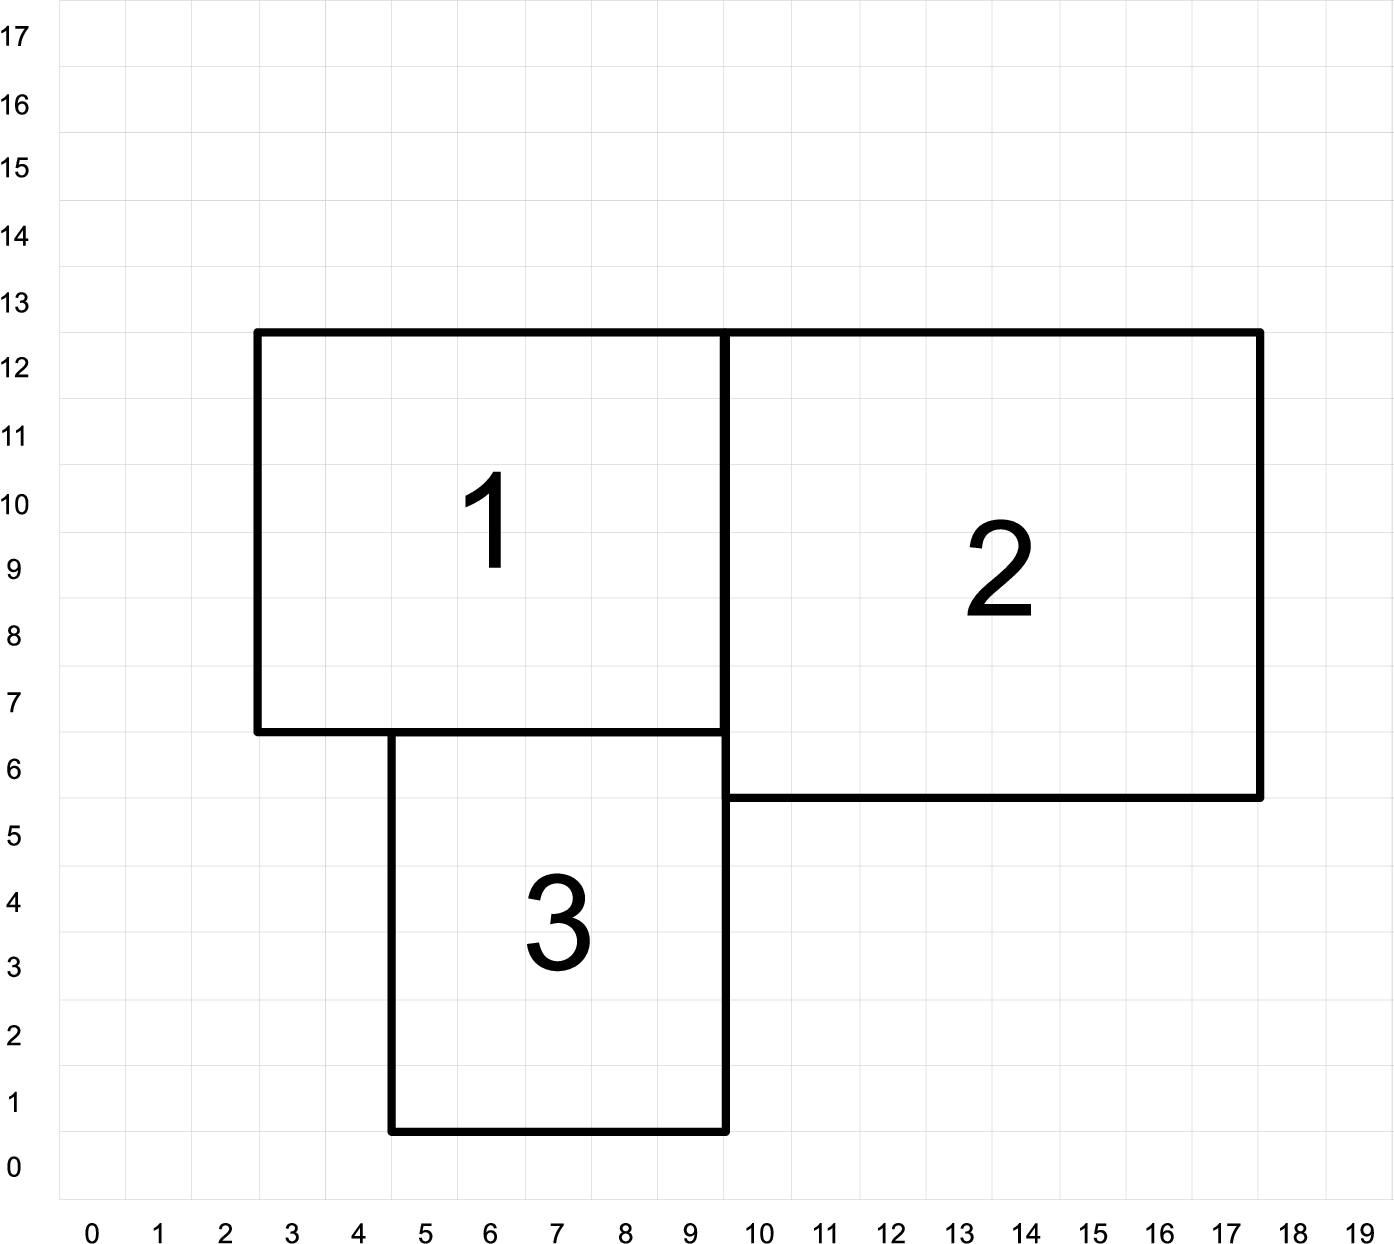
\includegraphics[width=4.0in]{index_grid2}
\caption[Single-level grid structure]
{\label{fig:soft:indexspace} Three boxes that comprise a single level.  At this
  resolution, the domain is 20$\times$18 zones.  Note that the
  indexing in \amrex\ starts with $0$.}
\end{figure}


A \code{\farraybox} or {\em FAB}, for {\em Fortran array box} is a data
structure that contains a \bbox\ locating it in space, as well as a
pointer to a data buffer.  The real floating point data are stored as
one-dimensional arrays in \farraybox es.  The associated \bbox can be
used to reshape the 1D array into multi-dimensional arrays to be used
by Fortran subroutines.  The key part of the \cpp\ \amrex\ data
structures is that this data buffer can be sent to Fortran, where it
will appear as a {\tt DIM}+1 dimensional array ({\tt DIM} space + 1
component).

Note: \castro\ is complied for a specific dimensionality.


\subsection{\multifab}

At the highest abstraction level, we have the \code{\multifab} (mulitple
\farraybox es).  A \multifab\ contains an array of \bbox es, including
\bbox es owned by other processors for the purpose of communication,
an array of MPI ranks specifying which MPI processor owns each \bbox,
and an array of pointers to \farraybox es owned by this MPI
processor. \MarginPar{is this still an accurate description?}  Note: a
\multifab\ is a collection of the boxes that together make up a single
level of data in the AMR hierarchy.

A \multifab\ can have multiple components (like density, temperature,
...) as well as a perimeter of ghost cells to exchange data with
neighbors or implement boundary conditions (this is all reflected in
the underlying \farraybox).

Parallelization in \amrex\ is done by distributing the FABs across
processors.  Each processor knows which FABs are local to it.  To loop
over all the boxes local to a processor, an \mfiter\ is used (more
on this below).

High-level operations exist on \multifab s to add, subtract, multiply,
etc., them together or with scalars, so you don't need to write out
loops over the data directly.

In \castro, \multifab s are one of the main data structures you will
interact with in the \cpp\ portions of the code.


\subsection{\statedata}

\label{soft:sec:statedata}

\code{\statedata} is a class that essentially holds a pair of \multifab s: one
at the old time and one at the new time.  \amrex\ knows how to
interpolate in time between these states to get data at any
intermediate point in time.  The main data that we care about in
\castro\ (the fluid state, gravitational potential, etc.) will be
stored as \statedata.  Essentially, data is made \statedata\ in
\castro\ if we need it to be stored in checkpoints / plotfiles, and/or
we want it to be automatically interpolated when we refine.

An \amrlevel\ stores an array of \statedata\ (in a \cpp\ array
called {\tt state}).  We index this array using integer keys (defined
via an {\tt enum} in {\tt Castro.H}).  The state data is registered
with \amrex\ in \code{Castro\_setup.cpp}.

Note that each of the different \statedata\ carried in the {\tt state}
array can have different numbers of components, ghost cells, boundary
conditions, etc.  This is the main reason we separate all this data
into separate \statedata\ objects collected together in an indexable
array.

The current \statedata\ names  \castro\ carries are:
\begin{itemize}
\item \variable{State\_Type} : this is the {\tt NUM\_STATE} hydrodynamics
  components that make up the conserved hydrodynamics state (usually
  referred to as $\Ub$ in these notes.  But note that this does
  not include the radiation energy density.

  In Fortran, the components of a FAB derived from {\tt State\_Type}
  is indexed using the integer keys defined in \code{Castro\_nd.F90}
  and stored in \code{meth\_params\_module}, e.g., {\tt URHO}, {\tt UMX},
  {\tt UMY}, ...

  Note: regardless of dimensionality, we always carry around all
  three velocity components.  The ``out-of-plane'' components
  will simply be advected, but we will allow rotation (in particular,
  the Coriolis force) to affect them.

  {\tt State\_Type} \multifab s have no ghost cells by default for
  pure hydro and a single ghost cell by default when {\tt RADIATION}
  is enabled.  There is an option to force them to have ghost cells by
  setting the parameter \runparam{castro.state\_nghost} at runtime.

  Note that the prediction of the hydrodynamic state to the interface
  will require 4 ghost cells.  This accomodated by creating a separate
  \multifab, \variable{Sborder} that lives at the old-time level and
  has the necessary ghost cells.  We will describe this more later.

\item \variable{Rad\_Type} : this stores the radiation energy density,
  commonly denoted $E_r$ in these notes.  It has \variable{nGroups}
  components---the number of energy groups used in the multigroup
  radiation hydrodynamics approximation. \MarginPar{not sure how
    neutrinos factor in here}

\item \variable{PhiGrav\_Type} : this is simply the gravitational
  potential, usually denoted $\Phi$ in these notes.

\item \variable{Gravity\_Type} : this is the gravitational
  acceleration. There are always 3 components, regardless of the
  dimensionality (consistent with our choice of always carrying all 3
  velocity components).

\item \variable{PhiRot\_Type} : this is the rotational potential.
  When rotation is enabled, this will store the effective potential
  corresponding to the centrifugal force. 

\item \variable{Rotation\_Type} : this is the rotational acceleration.
  There are always 3 components, regardless of the dimensionality
  (consistent with our choice of always carrying all 3 velocity
  components).  This includes the terms corresponding to the Coriolis
  force, the centrifugal force, as well as optional terms due to the
  change in rotation rate, $\Omega$.

\item \variable{Source\_Type} : this holds the time-rate of change of
  the source terms, $d\Sb/dt$, for each of the {\tt NUM\_STATE} {\tt
    State\_Type} variables.

  \MarginPar{SDC does differently}

  Note: we do not make use of the old-time quantity here. In fact, we
  never allocate the \farraybox s for the old-time in the {\tt Source\_Type}
  \statedata, so there is not wasted memory.

\item \variable{Reactions\_Type} : this holds the data for the nuclear
  reactions.  It has {\tt NumSpec+2} components: the species
  creation rates (usually denoted $\omegadot_k$ in these notes),
  the specific energy generation rate ($\dot{e}_\mathrm{nuc}$),
  and its density ($\rho \dot{e}_\mathrm{nuc}$).  

  These are stored as \statedata\ so we have access to the reaction terms
  outside of advance, both for diagnostics (like flame speed estimation)
  and for reaction timestep limiting (this in particular needs the 
  data stored in checkpoints for continuity of timestepping upon restart).

\MarginPar{why do we need rho edot and edot separately?}

\item \variable{SDC\_Source\_Type} : this is used with the SDC
  time-advancement algorithm (not the default Strang-splitting
  algorithn).  This will store the {\tt NUM\_STATE} advective source
  terms for use in the evolution of the reactive terms in the SDC
  advancement.

\item \variable{SDC\_React\_Type} : this is used with the SDC
  time-advancement algorithm.  This stores the {\tt QVAR} terms
  that describe how the primitive variables change over the timestep
  due only to reactions.  These are used when predicting the interface
  states of the primitive variables for the hydrodynamics portion of the
  algorithm.

\end{itemize}

We access the multifabs that carry the data of interest by interacting
with the \statedata\ using one of these keys.  For instance:
\begin{lstlisting}
MultiFab& S_new = get_new_data(State_Type);
\end{lstlisting}
gets a pointer to the multifab containing the hydrodynamics state data
at the new time.


\subsection{Various source \multifab s}

There are a number of different \multifab s (and arrays of \multifab s)
that hold source term information.

\begin{itemize}

\item \variable{hydro\_source} : this is a \multifab\ that holds the
  update to the hydrodynamics (basically the divergence of the
  fluxes).  This is filled in the conservative update routine of the
  hydrodynamics.

  As this is expressed as a source term, what is actually stored is
  \begin{equation}
    \Sb_\mathrm{flux} = -\nabla \cdot {\bf F}
  \end{equation}
  So the update of the conserved state appears as:
  \begin{equation}
    \frac{\partial \Ub}{\partial t} = \Sb_\mathrm{flux}
  \end{equation}

\item \variable{old\_sources} : this is an array of \multifab s, with
  each \multifab\ with {\tt NUM\_STATE} components (e.g., one for each
  of our conservative state variables).  There are \variable{num\_src}
  \multifab s in the array, corresponding to the sponge, external
  sources, diffusion, hybrid momentum, gravity, and rotation.

  Each of the different physical processes will store the
  old-time-level source in its respective \multifab.  This makes it
  easy to sum over all of the physical processes to get a single
  source that affects a particular state variable.

\item \variable{new\_sources} : the correction to the sources to
  time-center the source update.  This is the counterpart to
  {\tt old\_sources}.

  The general idea is that for a source component {\tt k}, then {\tt
    old\_source[k]} + {\tt new\_source[k]} should give an approximation
  to $S_k^{n+1/2}$.

  Generally this is accomplished by setting {\tt new\_source[k]} to
  $(S_k^{n+1} - S_k^{n})/2$.  For gravity, since we adopt a conservative
  formulation using the time-centered fluxes the form is slightly
  different.

\item \variable{sources\_for\_hydro} : a single \multifab\ that stores
  the sum of sources over each physical process (from {\tt
    old\_sources} or {\tt new\_sources})

\end{itemize}

\section{\mfiter\ and interacting with Fortran}

The process of looping over boxes at a given level of refinement and
operating on their data in Fortran is linked to how \castro\ achieves
thread-level parallelism.  The OpenMP approach in \castro\ has evolved
considerably since the original paper was written, with the modern
approach, called {\em tiling}, gearing up to meet the demands of
many-core processors in the next-generation of supercomputers.  We
discuss the original and new approach together here.

In both cases, the key construct is the \code{\mfiter}---this is a
\cpp\ iterator that knows how to loop over the \farraybox es in the
\multifab\ that are local to the processor (in this way, a lot of the
parallelism is hidden from view).

\subsection{Non-Tiling \mfiter}

The non-tiling way to iterate over the \farraybox s is
\footnote{Note: some older code will use a special \amrex\ preprocessor macro,
\code{BL\_TO\_FORTRAN}, defined in \code{ArrayLim.H}, that converts
the \cpp\ multifab into a Fortran array and its {\tt lo} and {\tt hi} indices.
Additionally, some older code will wrap the Fortran subroutine name
in an additional preprocessor macro, \code{BL\_FORT\_PROC\_CALL}
to handle the name mangling between Fortran and C.  This later
macro is generally not needed any more because of Fortran 2003
interoperability with C (through the Fortran {\tt bind} keyword).
}:
\begin{lstlisting}[language=C++]
  for (MFIter mfi(mf); mfi.isValid(); ++mfi) // Loop over boxes
  {
    // Get the index space of this iteration
    const Box& box = mfi.validbox();

    // Get a reference to the FAB, which contains data and box
    FArrayBox& fab = mf[mfi];

    // Get the index space for the data region in th FAB.
    // Note "abox" may have ghost cells, and is thus larger than
    // or equal to "box" obtained using mfi.validbox().
    const Box& abox = fab.box();

    // We can now pass the information to a Fortran routine,
    // fab.dataPtr() gives a double*, which is reshaped into
    // a multi-dimensional array with dimensions specified by
    // the information in "abox". We will also pass "box",
    // which specifies our "work" region.
    do_work(ARLIM_3D(box.loVect()), ARLIM_3D(box.hiVect()),
            fab.dataPtr(), fab.nComp(),
            ARLIM_3D(abox.loVect()), ARLIM_3D(abox.hiVect())

  }
\end{lstlisting}
A few comments about this code
\begin{itemize}
\item In this example, we are working off of a \multifab\ named {\tt mf}.
  This could, for example, come from state data as:
\begin{lstlisting}
 MultiFab& mf = get_old_data(State_Type);
\end{lstlisting}

\item We are passing the data in {\tt mf} one box at a time to the
  Fortran function {\tt do\_work}.

\item Here the \mfiter\ iterator, {\tt mfi}, will perform the loop
  only over the boxes that are local to the MPI task.  If there are 3
  boxes on the processor, then this loop has 3 iterations.

  {\tt ++mfi} iterates to the next \farraybox\ owned by the
  \multifab\ {\tt mf}, and {\tt mfi.isValid()} returns {\tt false}
  after we've reached the last box contained in the MultiFab,
  terminating the loop.

\item {\tt box} as returned from {\tt mfi.validbox()} does not include
   ghost cells.  This is the valid data region only.
   We can get the indices of the valid zones as {\tt box.loVect()} and
   {\tt box.hiVect()}.

   In passing to the Fortran function, we use the macro
   \code{ARLIM\_3D}, defined in \code{ArrayLim.H} to pass the {\tt lo}
   and {\tt hi} vectors as pointers to an {\tt int} array.  This array
   is defined to always be 3D, with {\tt 0}s substituted for the
   higher dimension values if we are running in 1- or 2D.

   Passing the data in this 3D fashion is a newer approach in \castro.
   This enables writing {\em dimension agnostic code}.  There are many
   other approaches that will pass only the {\tt DIM} values of {\tt
     lo} and {\tt hi} using alternate macros in {\tt ArrayLim.H}.

\item {\tt fab.dataPtr()} returns a {\tt double *}---a pointer to the
  data region.  This is what is passed to Fortran.

\item {\tt fab.nComp()} gives an {\tt int}---the number of components
  in the \multifab.  This will be used for dimensioning in Fortran.

\item To properly dimension the array in Fortran, we need the actual
  bounds of the data region, including any ghost cells.  This is the
  \bbox\ {\tt abox}, obtained as {\tt fab.box()}.  We pass the {\tt
    lo} and {\tt hi} of the full data region as well.

\end{itemize}

To properly compile, we need a prototype for the Fortran
function.  These are placed in the {\tt *\_F.H} files in the
\castro\ {\tt Source/} directory.  Here's the prototype for
our function:

\begin{lstlisting}[language=C++]
  void do_work
    (const int* lo, const int* hi,
     Real* state, const Real& ncomp
     const int* s_lo, const int* s_hi)
\end{lstlisting}

A few comments on the prototype:
\begin{itemize}
\item we use the {\tt const} qualifier on the many of the arguments.
  This indicates that the data that is pointed to cannot be
  modified\footnote{the way to read these complicated
    \cpp\ declarations is right-to-left.  So `const int* lo` means
    `lo` is a integer pointer to a memory space that is constant.  See
    \url{https://isocpp.org/wiki/faq/const-correctness\#ptr-to-const}}
    means that the pointers themselves are to be unmodified.  But the
    contents of the memory space that they point to can be modified.

\item For {\tt ncomp}, we in the calling sequence, we just did {\tt
  fab.nComp()}.  This returns a {\tt int}.  But Fortran is a
  pass-by-reference language, so we make the argument in the prototype
  a reference.  This ensures that it is passed by reference.
\end{itemize}

In our Fortran example, we want to loop over all of the data,
including 1 ghost cell all around.  The corresponding Fortran function
will look like:
\begin{lstlisting}[language=Fortran]
  subroutine do_work(lo, hi, &
                     state, ncomp, &
                     s_lo, s_hi) bind(C, name="do_work")

    use prob_params_module, only : dg

    integer, intent(in) :: lo(3), hi(3)
    integer, intent(in) :: s_lo(3), s_hi(3), ncomp

    real (kind=dp_t), intent(inout) :: state(s_lo(1):s_hi(1), &
                                             s_lo(2):s_hi(2), &
                                             s_lo(3):s_hi(3), ncomp)

    ! loop over the data
    do k = lo(3)-1*dg(3), hi(3)+1*dg(3)
       do j = lo(2)-1*dg(2), hi(2)+1*dg(2)
          do i = lo(1)-1*dg(1), hi(1)+1*dg(1)

             ! work on state(i,j,k,:), where the last index
             ! is the component of the multifab

          enddo
       enddo
    enddo

  end subroutine do_work
\end{lstlisting}

Finally, comments on the Fortran routine;
\begin{itemize}
\item We use the Fortran 2003 {\tt bind} keyword to specify
  that we want this to be interoperable with C.  Ordinarily
  we would not need to specify the optional argument {\tt name}
  in the binding, but the PGI compiler requires this if our
  Fortran subroutine is part of a module.

\item We dimension state using {\tt s\_lo} and {\tt s\_hi}---these are
  the bounds we got from the \farraybox, and are for the entire data
  region, including ghost cells.

  Note, in Fortran, the spatial indices of {\tt state} don't
  necessarily start at {\tt 1}---they reflect the global index space
  for the entire domain at this level of refinement.  This means that
  we know where the box is located.

  Later we'll see how to compute the spatial coordinates using this
  information.

\item Our loop uses {\tt lo} and {\tt hi}---these are the indices
  of the valid data region (no ghost cells).  Since we want a single
  ghost cell all around, we subtract {\tt 1} from {\tt lo} and add {\tt 1}
  to {\tt hi}.

  Finally, since this is dimension-agnostic code (it should work
  correctly in 1-, 2-, and 3D), we need to ensure the loops over the
  higher dimensions do nothing when we compile for a lower
  dimensionality.  This is the role of {\tt dg}---{\tt dg} is {\tt 1}
  if our simulation includes that spatial dimension and {\tt 0}
  otherwise.

  If we were not looping over ghost cells too, then we would not need
  to invoke {\tt dg}, since {\tt lo} and {\tt hi} are both set to {\tt
    0} for any dimensions not represented in our simulation.

\end{itemize}

Up to this point, we have not said anything about threading.  In this
style of using the \mfiter, we implement the OpenMP in Fortran, for
instance by putting a pragma around the outer loop in this example.


\subsection{\amrex's Current Tiling Approach In C++}
\label{sec:boxlib1}

There are two types of tiling that people discuss.  In {\em logical
tiling}, the data storage in memory is unchanged from how we do things
now in pure MPI.  In a given box, the data region is stored
contiguously).  But when we loop in OpenMP over a box, the tiling
changes how we loop over the data.  The alternative is called {\em
separate tiling}---here the data storage in memory itself is changed
to reflect how the tiling will be performed.  This is not considered
in \amrex.

We have recently introduced logical tiling into parts of \amrex\.  It
is off by default, to make the transition smooth and because not
everything should be tiled.  It can be enabled on a loop-by-loop basis
by setting an optional argument to \mfiter.  We demonstrate this
below.  Further examples can be found at {\tt Tutorials/Tiling\_C},
and {\tt Src/LinearSolvers/C\_CellMG/}.

In our logical tiling approach, a box is logically split into tiles,
and a {\tt MFIter} loops over each tile in each box.  Note that the
non-tiling iteration approach can be considered as a special case of
tiling with the tile size equal to the box size.

Let us consider an example.  Suppose there are four boxes---see
Figure~\ref{fig:domain-tiling}.
\begin{figure}[t]
\centering
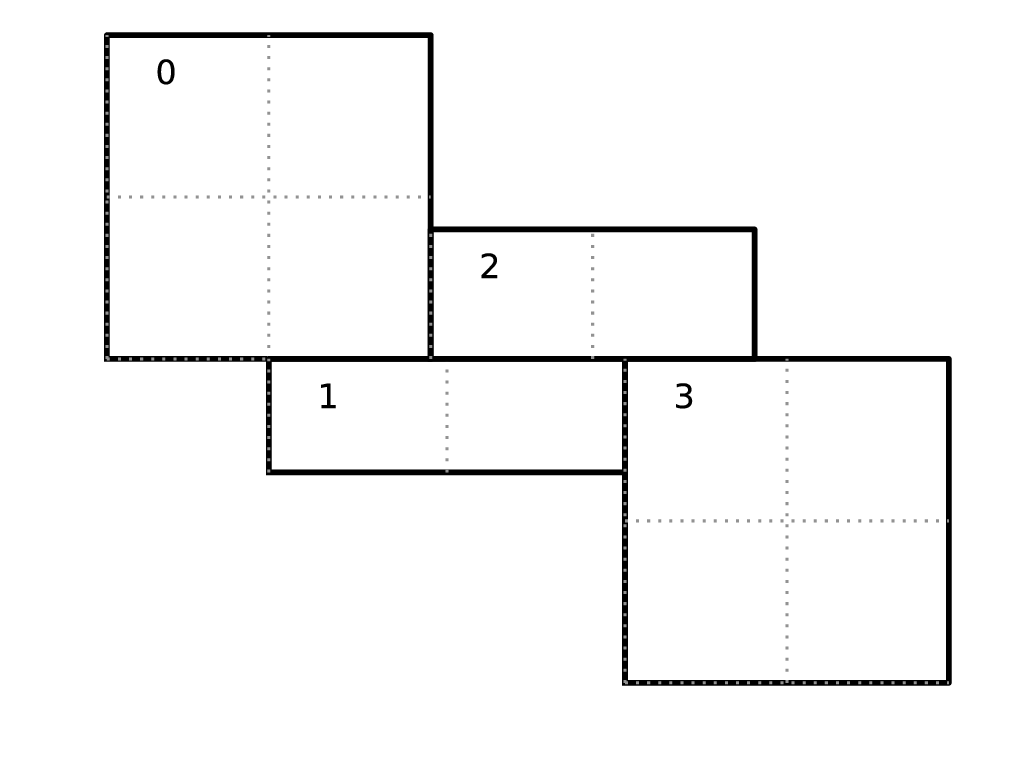
\includegraphics[width=0.8\linewidth]{domain-tile}
\caption{\label{fig:domain-tiling} A simple domain showing 4
  {\tt Box}es labeled 0--3, and their tiling regions (dotted lines)}
\end{figure}
%
The first box is divided into 4 logical tiles, the second and third
are divided into 2 tiles each (because they are small), and the fourth
into 4 tiles.  So there are 12 tiles in total.  The difference between
the tiling and non-tiling version are then:

\begin{itemize}
\item In the tiling version, the loop body will be run 12 times.  Note
  that {\tt tilebox} is different for each tile, whereas {\tt fab}
  might be referencing the same object if the tiles belong to the same
  box.

\item In the non-tiling version (by constructing {\tt MFIter} without
  the optional second argument or setting to {\tt false}), the loop
  body will be run 4 times because there are four boxes, and a call to
  {\tt mfi.tilebox()} will return the traditional {\tt validbox}.  The
  non-tiling case is essentially having one tile per box.
\end{itemize}


The tiling implementation of the same call to our the Fortran {\tt
  do\_work} routine is show below:

\begin{lstlisting}[language=C++]
  bool tiling = true;
  for (MFIter mfi(mf, tiling); mfi.isValid(); ++mfi) // Loop over tiles
  {
    // Get the index space of this iteration.
    const Box& box = mfi.growntilebox(1);

    // Get a reference to the FAB, which contains data and box
    FArrayBox& fab = mf[mfi];

    // Get the index space for the data pointed by the double*.
    const Box& abox = fab.box();

    // We can now pass the information to a Fortran routine.
    do_work(ARLIM_3D(box.loVect()), ARLIM_3D(box.hiVect()),
            fab.dataPtr(), fab.nComp(),
            ARLIM_3D(abox.loVect()), ARLIM_3D(abox.hiVect())

  }
\end{lstlisting}
Note that the code is almost identical to the one in \S~\ref{sec:boxlib0}.
Some comments:
\begin{itemize}
\item The iterator now takes an extra argument to turn on tiling (set
  to {\tt true}).  

  There is another interface fo {\tt MFIter} that can take an {\tt
    IntVect} that explicitly gives the tile size in each coordinate
  direction.  If we don't explictly specify the tile size at the loop,
  then the runtime parameter \runparam{fabarray.mfiter\_tile\_size}
  can be used to set it globally.

\item {\tt .validBox()} has the same meaning as in the non-tile
  approach, so we don't use it.  
  Since in this example, we want to include a single ghost cell in our
  loop over the data, we use {\tt .growntilebox(1)} (where the {\tt 1}
  here indicates a single ghost cells) to get the {\tt Box} (and
  corresponding {\tt lo} and {\tt hi}) for the {\em current tile}, not
  the entire data region.  If instead, we just wanted the valid
  region in Fortran, without any ghost cells, we would use {\tt
    .tilebox()}.

\item When passing into the Fortran routine, we still use the index
  space of the entire \farraybox\ (including ghost cells), as seen in
  the {\tt abox} construction.  This is needed to properly dimension
  the array in Fortran.  

  The Fortran routine will declare a multidimensional array that is of
  the same size as the entire box, but only work on the index space
  identified by the tile-box ({\tt box}).
\end{itemize}

The Fortran code is almost the same as before, but now our loop 
simply uses {\tt lo} and {\tt hi}, since, by construction with
{\tt .growntilebox(1)}, this already includes the single ghost cell 
all around:
\begin{lstlisting}[language=Fortran]
  subroutine do_work(lo, hi, &
                     state, ncomp, &
                     s_lo, s_hi) bind(C, name="do_work")

    integer, intent(in) :: lo(3), hi(3)
    integer, intent(in) :: s_lo(3), s_hi(3), ncomp

    real (kind=dp_t), intent(inout) :: state(s_lo(1):s_hi(1), &
                                             s_lo(2):s_hi(2), &
                                             s_lo(3):s_hi(3), ncomp)

    ! loop over the data
    do k = lo(3), hi(3)
       do j = lo(2), hi(2)
          do i = lo(1), hi(1)

             ! work on state(i,j,k,:), where the last index
             ! is the component of the multifab

          enddo
       enddo
    enddo

  end subroutine do_work
\end{lstlisting}

The function prototype is unchanged.

Tiling provides us the opportunity of a coarse-grained approach for
OpenMP.  Threading can be turned on by inserting the following line
above the {\tt for (MFIter...)} line.
\begin{lstlisting}
  #pragma omp parallel
\end{lstlisting}
Note that the OpenMP pragma does not have a {\tt for}---this is not
used when working with an iterator.

Assuming four threads are used in the above example, thread 0 will
work on 3 tiles from the first box, thread 1 on 1 tile from the first
box and 2 tiles from the second box, and so forth.  Note that
OpenMP can be used even when tiling is turned off.  In that case, the
OpenMP granularity is at the box level (and good performance would need
many boxes per MPI task).

The tile size for the three spatial dimensions can be set by a
parameter, e.g., {\tt fabarray.mfiter\_tile\_size = 1024000 8 8}.  A
huge number like {\tt 1024000} will turn off tiling in that direction.
As noted above, the {\tt MFIter} constructor can also take an explicit
tile size: {\tt MFIter(mfi(mf,IntVect(128,16,32)))}.

Note that tiling can naturally transition from all threads working
on a single box to each thread working on a separate box as the boxes
coarsen (e.g., in multigrid).

The {\tt MFIter} class provides some other useful functions:
\begin{itemize}
  \item {\tt mfi.validbox()} : The same meaning as before independent of tiling.

  \item {\tt mfi.tilebox()} : The standard way of getting the bounds of the 
    current tile box.  This will tile over the valid data region only.

  \item {\tt mfi.growntilebox(int)} : A grown tile box that includes
    ghost cells at box boundaries only.  Thus the returned boxes for a
    \farraybox\ are non-overlapping.

  \item {\tt mfi.nodaltilebox(int)} : Returns non-overlapping
    edge-type boxes for tiles.  The argument is for direction.

  \item {\tt mfi.fabbox()}  : Same as mf[mfi].box().
\end{itemize}

Finally we note that tiling is not always desired or better.  The
traditional fine-grained approach coupled with dynamic scheduling is
more appropriate for work with unbalanced loads, such as chemistry
burning in cells by an implicit solver.  Tiling can also create extra
work in the ghost cells of tiles.


\subsubsection{Practical Details in Working with Tiling}

With tiling, the OpenMP is now all in \cpp, and not in Fortran for all
modules except reactions and {\tt initdata}.  

It is the responsibility of the coder to make sure that the routines
within a tiled region are safe to use with OpenMP.  In particular,
note that:
\begin{itemize}
\item tile boxes are non-overlapping
\item the union of tile boxes completely cover the valid region of the
  fab
\item Consider working with a node-centered MultiFab, {\tt ugdnv}, and
  a cell-centered MultiFab, {\tt s}:
  \begin{itemize}

  \item with {\tt mfi(s)}, the tiles are based on the cell-centered
    index space.  If you have an $8\times 8$ box, then and 4 tiles,
    then your tiling boxes will range from $0\rightarrow 3$,
    $4\rightarrow 7$.

  \item with {\tt mfi{ugdnv}}, the tiles are based on nodal indices,
    so your tiling boxes will range from $0\rightarrow 3$,
    $4\rightarrow 8$.

  \end{itemize}

\item When updating routines to work with tiling, we need to
  understand the distinction between the index-space of the entire box
  (which corresponds to the memory layout) and the index-space of the
  tile.

  \begin{itemize}

  \item In the \cpp\ end, we pass (sometimes via the {\tt
    BL\_TO\_FORTRAN()} macro) the {\tt loVect} and {\tt hiVect} of the
    entire box (including ghost cells).  These are then used to
    allocate the array in Fortran as:
\begin{lstlisting}
  double precision :: a(a_l1:a_h1, a_l2:a_h2, ...)
\end{lstlisting}
    When tiling is used, we do not want to loop as {\tt do a\_l1,
      a\_h1}, but instead we need to loop over the tiling region.  The
    indices of the tiling region need to be passed into the Fortran
    routine separately, and they come from the {\tt mfi.tilebox()}
    or {\tt mfi.growntilebox()} statement.

  \item In Fortran, when initializing an array to {\tt 0}, do so only
    over the tile region, not for the entire box.  For a Fortran array
    {\tt a}, this means we cannot do:
\begin{lstlisting}
  a = 0.0
  a(:,:,:,:) = 0.0
\end{lstlisting}
    but instead must do:
\begin{lstlisting}
  a(lo(1):hi(1),lo(2):hi(2),lo(3):hi(3),:) = 0.0
\end{lstlisting}
    where {\tt lo()} and {\tt hi()} are the index-space for the tile box
    returned from {\tt mfi.tilebox()} in \cpp\ and passed into the Fortran
    routine.

\item Look at {\tt r\_old\_s} in {\tt Exec/gravity\_tests/DustCollapse/probdata.f90} as an
  example of how to declare a {\tt threadprivate} variable---this is then used
  in {\tt sponge\_nd.f90}.

\end{itemize}

\end{itemize}



\section{Boundaries: {\tt FillPatch} and {\tt FillPatchIterator}}

\amrex\ calls the act of filling ghost cells a {\em fillpatch}
operation.  Boundaries between grids are of two types. The first we
call ``fine-fine'', which is two grids at the same level.  The second
type is "coarse-fine", which needs interpolation from the coarse grid
to fill the fine grid ghost cells.  Both of these are part of the
fillpatch operation.  Fine-fine fills are just a straight copy from
``valid regions'' to ghost cells.  Coarse-fine fills are enabled
because the \statedata\ is not just arrays, they're ``State Data'',
which means that the data knows how to interpolate itself (in an
anthropomorphical sense).  The type of interpolation to use is defined
in {\tt Castro\_setup.cpp}---search for {\tt
  cell\_cons\_interp}, for example---that's ``cell conservative
interpolation'', i.e., the data is cell-based (as opposed to
node-based or edge-based) and the interpolation is such that the
average of the fine values created is equal to the coarse value from
which they came.  (This wouldn't be the case with straight linear
interpolation, for example.)

Additionally, since \statedata\ has an old and new timelevel, 
the fill patch operation can interpolate to an intermediate time.

\subsection{Examples}

To illustrate the various ways we fill ghost cells and use the data,
let's consider the following scenarios:


\begin{itemize}

\item {\em You have state data that was defined with no ghost cells.  You
  want to create a new \multifab\ containing a copy of that data with
  {\tt NGROW} ghost cells.}

  This is the case with \variable{Sborder}---the \multifab\ of the
  hydrodynamic state that we use to kick-off the hydrodynamics 
  advance.

  {\tt Sborder} is declared in {\tt Castro.H} simply as:
\begin{lstlisting}[language=C++]
  Multifab Sborder;
\end{lstlisting}

  It is then allocated in \code{Castro::initialize\_do\_advance()}
\begin{lstlisting}[language=C++]
  Sborder.define(grids, NUM_STATE, NUM_GROW, Fab_allocate);                   
  const Real prev_time = state[State_Type].prevTime();                        
  expand_state(Sborder, prev_time, NUM_GROW);      
\end{lstlisting}
  Note in the call to {\tt .define()}, we tell \amrex\ to already
  allocate the data regions for the \farraybox s that are part of {\tt
    Sborder}.

  The actually filling of the ghost cells is done by
  \code{Castro::expand\_state()}:
\begin{lstlisting}[language=C++]
  AmrLevel::FillPatch(*this, Sborder, NUM_GROW, 
                      prev_time, State_Type, 0, NUM_STATE);                
\end{lstlisting}
  Here, we are filling the {\tt ng} ghost cells of \multifab {\tt
    Sborder} at time {\tt prev\_time}.  We are using the
  \statedata\ that is part of the current {\tt Castro} object that we
  are part of.  Note: {\tt FillPatch} takes an object reference as its
  first argument, which is the object that contains the relevant
  \statedata---that is what the {\tt *this} pointer indicates.
  Finally, we are copying the {\tt State\_Type} data components 0 to
  {\tt NUM\_STATE}\footnote{for clarity and continuity in this
    documentation, some of the variable names have been changed
    compared to the actual code}.

The result of this operation is that {\tt Sborder} will now have
{\tt NUM\_GROW} ghost cells consistent with the {\tt State\_Type}
data at the old time-level.

\item {\em You have state data that was defined with {\tt NGROW} ghost
  cells.  You want to ensure that the ghost cells are filled
  (including any physical boundaries) with valid data.}

  This is very similar to the procedure shown above.  The main
  difference is that for the \multifab\ that will be the target
  of the ghost cell filling, we pass in a reference to the \statedata\
  itself.  

  The main thing you need to be careful of here, is that you 
  need to ensure that the the time you are at is consistent with
  the \statedata's time.  Here's an example from the radiation
  portion of the code {\tt MGFLDRadSolver.cpp}:

\begin{lstlisting}[language=C++]
  Real time = castro->get_state_data(Rad_Type).curTime();
  MultiFab& S_new = castro->get_new_data(State_Type);

  AmrLevel::FillPatch(*castro, S_new, ngrow, time, State_Type,
                      0, S_new.nComp(), 0); 
\end{lstlisting}

  In this example, {\tt S\_new} is a pointer to the new-time-level
  {\tt State\_Type} \multifab.  So this operation will use the {\tt
    State\_Type} data to fill its own ghost cells.  we fill the {\tt
    ngrow} ghost cells of the new-time-level {\tt State\_Type} data,
  for all the components.

  Note that in this example, because the \statedata\ lives in the {\tt
    Castro} object and we are working from the {\tt Radiation} object,
  we need to make reference to the current {\tt castro} object
  pointer.  If this were all done within the {\tt Castro} object, then
  the pointer will simply be {\tt *this}, as we saw above.

\item {\em You have a \multifab\ with some derived quantity.  You want to
  fill its ghost cells.}

  \multifab s have a {\tt FillBoundary()} method that will fill all
  the ghost cells between boxes at the same level.  It will not fill
  ghost cells at coarse-fine boundaries or at physical boundaries.  \MarginPar{what is the use case for this?}

\item {\em You want to loop over the FABs in state data, filling ghost cells
  along the way}

  This is the job of the \code{\fillpatchiterator}---this iterator is used to
  loop over the grids and fill ghostcells.  A key thing to keep in
  mind about the \fillpatchiterator\ is that you operate on a copy
  of the data---the data is disconnected from the original source.  If
  you want to update the data in the source, you need to explicitly
  copy it back.  Also note: {\tt FillPatchIterator} takes a multifab,
  but this is not filled---this is only used to get the grid
  layout.  Finally, the way the \fillpatchiterator\ is implemented
  is that all the communication is done first, and then the iterating
  over boxes commences.

  For example, the loop that calls {\tt CA\_UMDRV} (all the
  hydrodynamics integration stuff) starts with
\begin{lstlisting}
   for (FillPatchIterator fpi(*this, S_new, NUM_GROW,
                              time, State_Type, strtComp, NUM_STATE);
         fpi.isValid(); ++fpi)
   {
     FArrayBox &state = fpi();
     Box bx(fpi.validbox());

     // work on the state FAB.  The interior (valid) cells will 
     // live between bx.loVect() and bx.hiVect()
   }
\end{lstlisting}
Here the {\tt FillPatchIterator} is the thing that distributes the
grids over processors and makes parallel ``just work''. This fills the
single patch ``{\tt fpi}'' , which has {\tt NUM\_GROW} ghost cells,
with data of type ``{\tt State\_Type}'' at time ``{\tt time}'',
starting with component {\tt strtComp} and including a total of {\tt
  NUM\_STATE} components. \MarginPar{how do tiling and \fillpatchiterator\ work together?}

\end{itemize}

In general, one should never assume that ghostcells are valid, and
instead do a fill patch operation when in doubt.  Sometimes we will
use a \fillpatchiterator\ to fill the ghost cells into a multifab
without an explict look.  This is done as:
\begin{lstlisting}
  FillPatchIterator fpi(*this,S_old,1,time,State_Type,0,NUM_STATE);
  MultiFab& state_old = fpi.get_mf();     
\end{lstlisting}
In this operation, {\tt state\_old} points to the internal
\multifab\ in the \fillpatchiterator, by getting a reference to it as
              {\tt fpi.get\_mf()}.  This avoids a local copy.

Note that in the examples above, we see that only \statedata\ can fill
physical boundaries (because these register how to fill the boundaries
when they are defined).  There are some advanced operations in
\amrex\ that can get around this, but we do not use them in \castro.  \MarginPar{ok?}

\subsection{Physical Boundaries}

\label{soft:phys_bcs}

Physical boundary conditions are specified by an integer
index\footnote{the integer values are defined in \code{BC\_TYPES.H}} in
  the inputs file, using the \runparam{castro.lo\_bc} and
  \runparam{castro.hi\_bc} runtime parameters.  The generally
  supported boundary conditions are, their corresponding integer key,
  and the action they take for the normal velocity, transverse
  velocity, and generic scalar are shown in Table~\ref{table:castro:bcs}

The definition of the specific actions are:
\begin{itemize}
\item {\tt INT\_DIR}: data taken from other grids or interpolated

\item {\tt EXT\_DIR}: data specified on EDGE (FACE) of bndry

\item {\tt HOEXTRAP}: higher order extrapolation to EDGE of bndry

\item {\tt FOEXTRAP}: first order extrapolation from last cell in interior

\item {\tt REFLECT\_EVEN}: $F(-n) = F(n)$ true reflection from interior cells

\item {\tt REFLECT\_ODD}: $F(-n) = -F(n)$ true reflection from interior cells
\end{itemize}


The actual registration of a boundary condition action to a particular
variable is done in {\tt Castro\_setup.cpp}. At the top we define
arrays such as ``{\tt scalar\_bc}'', ``{\tt norm\_vel\_bc}'', etc,
which say which kind of bc to use on which kind of physical boundary.
Boundary conditions are set in functions like ``{\tt
  set\_scalar\_bc}'', which uses the {\tt scalar\_bc} pre-defined
arrays.  We also specify the name of the Fortran routine that
is responsible for filling the data there (e.g., \code{hypfill}).
These routines are discussed more below.


If you want to specify a value at a function (like at an inflow
boundary), then you choose an {\em inflow} boundary at that face of
the domain.  You then need to write the implementation code for this.
An example is the problem \problem{toy\_convect} which implements a
hydrostatic lower boundary (through its custom \code{bc\_fill\_?d.F90}
routines.

\begin{table}
\renewcommand{\arraystretch}{1.5}
\centering
\begin{tabular}{lllll}
{\bf name} & {\bf integer} & {\bf normal velocity} & {\bf transverse velocity} & {\bf scalars} \\
\hline
interior & 0 & {\tt INT\_DIR} & {\tt INT\_DIR} & {\tt INT\_DIR} \\
inflow   & 1 & {\tt EXT\_DIR} & {\tt EXT\_DIR} & {\tt EXT\_DIR} \\
outflow  & 2 & {\tt FOEXTRAP} & {\tt FOEXTRAP} & {\tt FOEXTRAP} \\
symmetry & 3 & {\tt REFLECT\_ODD} & {\tt REFLECT\_EVEN} & {\tt REFLECT\_EVEN} \\
slipwall & 4 & {\tt REFLECT\_ODD} & {\tt REFLECT\_EVEN} & {\tt REFLECT\_EVEN} \\
noslipwall & 5 & {\tt REFLECT\_ODD} & {\tt REFLECT\_EVEN} & {\tt REFLECT\_EVEN} \\
\hline
\end{tabular}
\caption[Physics boundary conditions in \castro]
  {\label{table:castro:bcs} Physical boundary conditions supported in \castro.  {\color{red} why does slipwall and noslipwall do the same thing?}}
\renewcommand{\arraystretch}{1.0}
\end{table}


\subsection{\fluxregister}

A \fluxregister\ holds face-centered data at the boundaries of a box.
It is composed of a set of \multifab s (one for each face, so 6 for
3D).  A \fluxregister\ stores fluxes at coarse-fine interfaces, 
and isused for the flux-correction step.



\section{Other \amrex\ Concepts}

There are a large number of classes that help define the structure of
the grids, metadata associate with the variables, etc.  A good way to
get a sense of these is to look at the {\tt .H} files in the {\tt
  amrex/Src/} directory.

\subsection{Geometry class}

There is a {\tt Geometry} object, \variable{geom} for each level as part of 
the {\tt Castro} object (this is inhereted through \amrlevel). \MarginPar{correct?}



\subsection{ParmParse class}


\subsection{Error Estimators}


\section{{\tt Gravity} class}

There is a single {\tt Gravity} object, {\tt gravity}, that is a
static class member of the {\tt Castro} object.  This means that all
levels refer to the same {\tt Gravity} object.

Within the {\tt Gravity} object, there are pointers to the {\tt Amr}
object (as {\tt parent}), and all of the \amrlevel s (as a \parray,
{\tt LevelData}).  The {\tt gravity} object gets the geometry
information at each level through the parent {\tt Amr} class.


The main job of the {\tt gravity} object is to provide the potential
and gravitation acceleration for use in the hydrodynamic sources.
Depending on the approximation used for gravity, this could mean
calling the \amrex\ multigrid solvers to solve the Poisson equation.




\section{Fortran Helper Modules}

There are a number of modules that make data available to the Fortran
side of \castro\ or perform other useful tasks.

\begin{itemize}

\item \code{bl\_constants\_module}:

  This provides double precision constants as Fortran parameters, like 
  {\tt ZERO}, {\tt HALF}, and {\tt ONE}.

\item \code{bl\_types}:

  This provides a double precision type, {\tt dp\_t} for use in
  Fortran.  This should be identical to {\tt double precision} on most
  architectures.

\item \code{extern\_probin\_module}:

  This module provides access to the runtime parameters for the
  microphysics routines (EOS, reaction network, etc.).  The source
  for this module is generated at compile type via a {\tt make} rule
  that invokes a python script.  This will search for all of the 
  \code{\_parameters} files in the external sources, parse them 
  for runtime parameters, and build the module.
  

\item {\tt fundamental\_constants\_module}:

  This provides the CGS values of many physical constants.

\item {\tt math\_module}: 

  This provides simple mathematical functions.  At the moment, a cross
  product routine.

\item {\tt meth\_params\_module}:

  This module provides the integer keys used to access the state
  arrays for both the conserved variables ({\tt URHO}, {\tt UMX}, $\ldots$)
  and primitive variables ({\tt QRHO}, {\tt QU}, $\ldots$), as well
  as the number of scalar variables.

  It also provides the values of most of the {\tt castro.{\em xxxx}}
  runtime parameters.

\item {\tt model\_parser\_module}:

  This module is built if {\tt USE\_MODELPARSER = TRUE} is set in the
  problem's {\tt GNUmakefile}.  It then provides storage for the an
  initial model and routines to read it in and interpolate onto the
  \castro\ grid.

\item {\tt prob\_params\_module}:

  \label{soft:prob_params}

  This module stores information about the domain and current level,
  and is periodically synced up with the \cpp\ driver.  The information
  available here is:
  \begin{itemize}
  \item \variable{physbc\_lo}, \variable{physbc\_hi}: these are the boundary
    condition types at the low and high ends of the domain, for each
    coordinate direction.  Integer keys, {\tt Interior}, {\tt Inflow},
    {\tt Outflow}, {\tt Symmetry}, {\tt SlipWall}, and {\tt
      NoSlipWall} allow you to interpret the values.

  \item \variable{center} is the center of the problem.  Note---this is up
    to the problem setup to define (in the {\tt probinit} subroutine).
    Alternately, it can be set at runtime via
    \runparam{castro.center}. \MarginPar{which wins if both try to set
      it?}

    Usually {\tt center} will be the physical center of the domain,
    but not always.  For instance, for axisymmetric problems, {\tt
      center} may be on the symmetry axis.

    {\tt center} is used in the multipole gravity, hybrid advection
    algorithm, rotation sources, for the point mass gravity, in
    defining the center of the sponge, and in deriving the radial
    velocity.  \MarginPar{other important places?}

  \item \variable{coord\_type}

  \item \variable{dim}

  \item \variable{dg}

  \item {\em refining information}

  \end{itemize}

\end{itemize}



\section{Setting Up Your Own Problem}

To define a new problem, we create a new directory in one
of the subdirectories of {\tt Exec/},
and place in it a {\tt Prob\_2d.f90} file (or {\tt 1d}/{\tt 3d},
depending on the dimensionality of the problem), a {\tt probdata.f90}
file, the {\tt inputs} and {\tt probin} files, and a {\tt
  Make.package} file that tells the build system what problem-specific
routines exist.  Finally, if you need custom boundary conditions, a
{\tt bc\_fill\_2d.F90} (or {\tt 1d}/{\tt 3d}) file is needed.  The
simplest way to get started is to copy these files from an existing
problem.  Here we describe how to customize your problem.

The purpose of these files is:
\begin{itemize}
\item \code{probdata.f90}: this holds the {\tt probdata\_module} Fortran module
  that allocates storage for all the problem-specific runtime parameters that
  are used by the problem (including those that are read from the {\tt probin}
  file.

\item \code{Prob\_?d.f90}: this holds the main routines to
  initialize the problem and grid and perform problem-specific boundary
  conditions:

  \begin{itemize}
  \item {\tt probinit()}:

    This routine is primarily responsible for reading in the {\tt
      probin} file (by defining the {\tt \&fortin} namelist and
    reading in an initial model (usually through the {\tt
      model\_parser\_module}---see the {\tt toy\_convect} problem
    setup for an example).  The parameters that are initialized
    here are those stored in the {\tt probdata\_module}.

  \item \code{ca\_initdata()}:

    This routine will initialize the state data for a single grid.
    The inputs to this routine are:
    \begin{itemize}
    \item {\tt level}: the level of refinement of the grid we are filling

    \item {\tt time}: the simulation time

    \item {\tt lo()}, {\tt hi()}: the integer indices of the box's {\em
      valid data region} lower left and upper right corners.  These
      integers refer to a global index space for the level and
      identify where in the computational domain the box lives.

    \item {\tt nscal}: the number of scalar quantities---this is not typically
      used in \castro.

    \item {\tt state\_l1}, {\tt state\_l2}, ({\tt state\_l3}): the
      integer indices of the lower left corner of the box in each
      coordinate direction.  These are for the box as allocated in memory,
      so they include any ghost cells as well as the valid data regions.

    \item {\tt state\_h1}, {\tt state\_h2}, ({\tt state\_h3}): the
      integer indices of the upper right corner of the box in each
      coordinate direction.  These are for the box as allocated in memory,
      so they include any ghost cells as well as the valid data regions.

    \item {\tt state()}: the main state array.  This is dimensioned as:
\begin{verbatim}
double precision state(state_l1:state_h1,state_l2:state_h2,NVAR)
\end{verbatim}
    (in 2-d), where {\tt NVAR} comes from the {\tt meth\_params\_module}.

    When accessing this array, we use the index keys provided by
    {\tt meth\_params\_module} (e.g., {\tt URHO}) to refer to specific
    quantities

    \item {\tt delta()}: this is an array containing the zone width ($\Delta x$)
      in each coordinate direction: $\mathtt{delta(1)} = \Delta x$,
      $\mathtt{delta(2)} = \Delta y$, $\ldots$.

    \item {\tt xlo()}, {\tt xhi()}: these are the physical coordinates of the
      lower left and upper right corners of the {\em valid region}
      of the box.  These can be used to compute the coordinates of the
      cell-centers of a zone as:
\begin{lstlisting}
  do j = lo(2), hi(2)
     y = xlo(2) + delta(2)*(dble(j-lo(2)) + 0.5d0)
     ...
\end{lstlisting}
     (Note: this method works fine for the problem initialization
     stuff, but for routines that implement tiling, as discussed below,
     {\tt lo} and {\tt xlo} may not refer to the same corner, and instead
     coordinates should be computed using {\tt problo()} from the {\tt
     prob\_params\_module}.)

    \end{itemize}
  \end{itemize}

\item \code{bc\_fill\_?d.F90}:

  These routines handle how \castro\ fills ghostcells {\em
  at physical boundaries} for specific data.  Most problem
  setups won't need to do anything special here, and inclusion
  of this file is optional -- only use it if you need to set
  specific boundary conditions.

  These routines are registered in {\tt Castro\_setup.cpp}, and
  called as needed.  By default, they just
  pass the arguments through to {\tt filcc}, which handles all of
  the generic boundary conditions (like reflecting, extrapolation,
  etc.).  The specific `{\tt fill}' routines can then supply the
  problem-specific boundary conditions, which are typically just
  Dirichlet boundary conditions (usually this means looking to see
  if the {\tt bc()} flag at a boundary is {\tt EXT\_DIR}.  The
  problem-specific code implementing these specific conditions
  should {\em follow} the {\tt filcc} call.

  \begin{itemize}
  \item {\tt ca\_hypfill}:
    This handles the boundary filling for the hyperbolic system.

  \item {\tt ca\_denfill}: At times, we need to fill just the density
    (always assumed to be the first element in the hyperbolic state)
    instead of the entire state.  When the fill patch routine is called
    with {\tt first\_comp = Density} and {\tt num\_comp = 1}, then we
    use {\tt ca\_denfill} instead of {\tt ca\_hypfill}.

    (Note: it seems that this may be used for more than just
    density, but it is only used for tagging and the plotfile)

  \item {\tt ca\_grav?fill}: These routines fill will the ghostcells
    of the gravitational acceleration grids with the gravitational
    acceleration.

    Note: for constant gravity, these routines will never be called.
    For one of the Poisson-type gravities, you only need to do
    something special here if you are implementing an {\tt Interior}
    boundary type (which you can test for by comparing {\tt
    bc(:,:,:)} to {\tt EXT\_DIR}.

    For the other standard physical boundary types, the ghost cell
    filling will be handled automatically by the default {\tt filcc}
    call in these routines.

    The gravitational acceleration in the ghost cells is used during
    the hydrodynamics portion of the code in predicting the
    interface states.

  \item {\tt ca\_reactfill}: This handles boundary filling for
    any {\tt Reactions\_Type} MultiFABs, which are sometimes used to interface
    with the nuclear burning module. It stores the normal state data
    in addition to components for the energy release and species change.

  \end{itemize}

  These routines take the following arguments:
  \begin{itemize}
  \item {\tt adv\_l1}, {\tt adv\_l2}, ({\tt adv\_l3}): the indicies of
    the lower left corner of the box holding the data we are working on.
    These indices refer to the entire box, including ghost cells.

  \item {\tt adv\_h1}, {\tt adv\_h2}, ({\tt adv\_h3}): the indicies of
    the upper right corner of the box holding the data we are working on.
    These indices refer to the entire box, including ghost cells.

  \item {\tt adv()}: the array of data whose ghost cells we are filling.
    Depending on the routine, this may have an additional index refering
    to the variable.

    This is dimensioned as:
\begin{verbatim}
  double precision adv(adv_l1:adv_h1,adv_l2:adv_h2)
\end{verbatim}

  \item {\tt domlo()}, {\tt domhi()}: the integer indices of the lower
    left and upper right corners of the valid region of the {\em entire
    domain}.  These are used to test against to see if we are filling
    physical boundary ghost cells.

    This changes according to refinement level: level-0 will
    range from {\tt 0} to {\tt castro.max\_grid\_size},
    and level-n will range from {\tt 0} to
    $\mathtt{castro.max\_grid\_size} \cdot \prod_n \mathtt{castro.ref\_ratio(n)}$.

  \item {\tt delta()}: is the zone width in each coordinate direction,
    as in {\tt initdata()} above.

  \item {\tt xlo()}: this is the physical coordinate of the lower
    left corner of the box we are filling---including the ghost cells.

    Note: this is different than how {\tt xlo()} was defined in
    {\tt initdata()} above.

  \item {\tt time}: the simulation time

  \item {\tt bc()}: an array that holds the type of boundary conditions
    to enforce at the physical boundaries for {\tt adv}.

    Sometimes it appears of the form {\tt bc(:,:)} and sometimes
    {\tt bc(:,:,:)}---the last index of the latter holds the variable
    index, i.e., density, pressure, species, etc.

    The first index is the coordinate direction and the second index
    is the domain face ({\tt 1} is low, {\tt 2} is hi), so {\tt
    bc(1,1)} is the lower $x$ boundary type, {\tt bc(1,2)} is
    the upper $x$ boundary type, {\tt bc(2,1)} is the lower
    $y$ boundary type, etc.

    To interpret the array values, we test against the quantities
    defined in {\tt bc\_types.fi} included in each subroutine,
    for example, {\tt EXT\_DIR}, {\tt FOEXTRAP}, $\ldots$.  The
    meaning of these are explained below.

  \end{itemize}

\end{itemize}


\subsection{Optional Files}

The follow problem-specific files are optional.  There are stubs for
each of these in the main source tree.  

\begin{itemize}

\item \code{Problem.f90} :

  This provides two routines, \code{problem\_checkpoint} and
  \code{problem\_restart} that can be used to add information to the
  checkpoint files and read it in upon restart.  This is useful for
  some global problem-specific quantities.  For instance, the
  \problem{wdmerger}\footnote{available separately at
    \url{https://github.com/BoxLib-Codes/wdmerger}} problem uses this
  to store center of mass position and velocity information in the
  checkpoint files that are used for runtime diagnostics.

  The name of the checkpoint directory is passed in as an argument.
  \code{Problem\_F.H} provides the \cpp\ interfaces for these routines.

\item \code{problem\_tagging\_?d.F90}, \code{problem\_tagging\_nd.F90}

  This implements problem-specific tagging for refinement, through a
  subroutine \code{set\_problem\_tags}.  The full hydrodynamic state
  ({\tt State\_Type}) is passed in, and the problem can mark zones for
  refinement by setting the \variable{tag} variable for a zone to
  \variable{set}.  An example is provided by the \problem{toy\_convect}
  problem which refines a rectangular region (fuel layer) based on
  a density parameter and the H mass fraction.

\item \code{Problem\_Derive\_F.H}, \code{Problem\_Derives.H}, \code{problem\_derive\_nd.f90}

  Together, these provide a mechanism to create derived quantities
  that can be stored in the plotfile.  {\tt Problem\_Derives.H}
  provides the \cpp\ code that defines these new plot variables.  It
  does this by adding them to the \variable{derive\_lst}---a list of
  derived variables that \castro\ knows about.\index{plotfiles!derived variables}  When adding new
  variables, a descriptive name, Fortran routine that does the
  deriving, and component of \statedata\ are specified.

  The Fortran routine that does the deriving is put in the
  problem-specific {\tt problem\_derive\_nd.f90} (and a prototype for
  \cpp\ is put in {\tt Problem\_Derives.H}).  A example is provided by
  the \problem{reacting\_bubble} problem, which derives several new
  quantities (perturbations against a background one-dimensional
  model, in this case).

\item \code{Prob.cpp}, \code{Problem.H}, \code{Problem\_F.H}

  These files provide problem-specific routines for computing global
  diagnostic information through the \code{sum\_integrated\_quantities}
  functionality that is part of the {\tt Castro} class.

  An example is provided by \problem{toy\_flame}, where an estimate
  of the flame speed is computed by integrating the mass of fuel on 
  the grid.

\end{itemize}



\subsection{Dimension Agnostic Problem Initialization}

Most of the problem setups have separate implementations for 1-, 2-,
and 3D.  A new method exists that allows you to write just a single
set of files for any dimensionality (this is called the {\em dimension
  agnostic} format).  To use this mode, set
\makevar{DIMENSION\_AGNOSTIC}{\tt = TRUE} in your {\tt GNUmakefile}.
Then write you problem initialization in \code{Prob\_nd.F90}.
Analogous routines exist for tagging and boundary conditions.  See the
\problem{rotating\_torus} and \problem{Noh} problem setups for an
example.

\section{Parallel I/O}

\label{software:io}

Both checkpoint files and plotfiles are really directories containing
subdirectories: one subdirectory for each level of the AMR hierarchy.
The fundamental data structure we read/write to disk is a MultiFab,
which is made up of multiple FAB's, one FAB per grid.  Multiple
MultiFabs may be written to each directory in a checkpoint file.
MultiFabs of course are shared across CPUs; a single MultiFab may be
shared across thousands of CPUs.  Each CPU writes the part of the
MultiFab that it owns to disk, but they don't each write to their own
distinct file.  Instead each MultiFab is written to a runtime
configurable number of files N (N can be set in the inputs file as the
parameter \runparam{amr.checkpoint\_nfiles} and \runparam{amr.plot\_nfiles}; the
default is 64).  That is to say, each MultiFab is written to disk
across at most N files, plus a small amount of data that gets written
to a header file describing how the file is laid out in those N files.

What happens is $N$ CPUs each opens a unique one of the $N$ files into
which the MultiFab is being written, seeks to the end, and writes
their data.  The other CPUs are waiting at a barrier for those $N$
writing CPUs to finish.  This repeats for another $N$ CPUs until all the
data in the MultiFab is written to disk.  All CPUs then pass some data
to CPU {\tt 0} which writes a header file describing how the MultiFab is
laid out on disk.

We also read MultiFabs from disk in a ``chunky'' manner, opening only $N$
files for reading at a time.  The number $N$, when the MultiFabs were
written, does not have to match the number $N$ when the MultiFabs are
being read from disk.  Nor does the number of CPUs running while
reading in the MultiFab need to match the number of CPUs running when
the MultiFab was written to disk.

Think of the number $N$ as the number of independent I/O pathways in
your underlying parallel filesystem.  Of course a ``real'' parallel
filesytem should be able to handle any reasonable value of $N$.  The
value {\tt -1} forces $N$ to the number of CPUs on which you're
running, which means that each CPU writes to a unique file, which can
create a very large number of files, which can lead to inode issues.


\chapter{Single-Level Flow Chart}
\input{FlowChart/FlowChart.tex}

\chapter{Runtime Parameters}
\label{chapter:parameters}

\section{Introduction to Runtime Parameters}

Castro has 2 sets of runtime parameters---those controlled by
\cpp\ and those controlled by Fortran.  The \cpp\ parameters are set
in the {\tt inputs} file and managed by the \amrex\ {\tt ParmParse}
class.  For \castro-specific parameters, we list the runtime
parameters in a file \code{\_cpp\_parameters} and generate the
\cpp\ code and headers using the \code{mk\_params.sh} script---note
this script needs to be run every time the {\tt \_cpp\_parameters}
file is updated.

The behavior of the network, EOS, and other microphysics routines are
controlled by a different set of runtime parameters.  These parameters are defined
in plain-text files \code{\_parameters} located in the different
directories that hold the microphysics code.  At compile time, a
script in the \amrex\ bulid system, \code{findparams.py}, locates all
of the {\tt \_parameters} files that are needed for the given choice
of network, integrator, and EOS, and assembles all of the runtime
parameters into a module named \code{extern\_probin\_module} (using the
\code{write\_probin.py} script).  The parameters are set in your {\tt
  probin} file in the {\tt \&extern} namelist.

\subsection{C++ parameter format}

The \cpp\ parameters take the form of:
\begin{verbatim}
# comment describing the parameter
name   type   default   need in Fortran?   ifdef    fortran name    fortran type
\end{verbatim}
Here, {\tt name} is the name of the parameter that will be looked for
in the {\tt inputs} file, {\tt type} is one of {\tt int}, {\tt Real},
or {\tt string}, and {\tt default} is the default value of the
parameter.  The next columns are optional, but you need to fill in all
of the information up to and including any of the optional columns you
need (e.g., if you are going to provide the {\tt fortran name}, you
also need to provide {\tt need in Fortran?} and {\tt ifdef}.  The {\tt
  need in Fortran?} column is {\tt y} if the runtime parameter should
be made available in Fortran (through \code{meth\_params\_module}).
The {\tt ifdef} field provides the name of a preprocessor name that
should wrap this parameter definition---it will only be compiled in if
that name is defined to the preprocessor.  The {\tt fortran name} is
the name that the parameter should use in Fortran---by default it will
be the same as {\tt name}.  The {\tt fortran type} is the data type of
the parameter in Fortran---by default it will be the
Fortran-equivalent to {\tt type}.  Finally, any comment immediately
before the parameter definition will be used to generate the \LaTeX\ documentation
describing the parameters.



\subsection{Microphysics/extern parameter format}

The microphysics/extern parameter definitions take the form of:
\begin{verbatim}
# comment describing the parameter
name              data-type       default-value      priority
\end{verbatim}
Here, the {\tt priority} is simply an integer.  When two directories
define the same parameter, but with different defaults, the version of
the parameter with the highest priority takes precedence.  This allows
specific implementations to override the general parameter defaults.

The documentation below for the \castro\ \cpp\ parameters is
automatically generated, using the comments in the {\tt \_cpp\_parameters}
file.



\section{Removed Runtime Parameters}

The following runtime parameters have been removed for \castro.
\begin{itemize}
\item {\tt castro.ppm\_flatten\_before\_integrals} : this parameter
  controlled whether we applied the flattening of the parabolic
  profiles before we integrated under their profiles or afterwards.
  The default was switched to flattening before the integration,
  which is more consistent with the original PPM methodology.  This
  parameter was removed since the variation enabled by this parameter
  was not that great. 

  (removed in commit: {\tt 9cab697268997714919de16db1ca7e77a95c4f98})


\item {\tt castro.ppm\_reference} and {\tt
  castro.ppm\_reference\_edge\_limit} : these parameters controlled
  whether we use the integral under the parabola for the fastest wave
  moving toward the interface for the reference state and whether in
  the case that the wave is moving away from the interface we use the
  cell-center value or the limit of the parabola on the interface.
  These were removed because there is little reason to not use the
  reference state.

  (removed in commit: {\tt 213f4ffc53463141084551c7be4b37a2720229aa})
\end{itemize}


\section{ {\tt castro } Namespace}

\label{ch:parameters}


%%%%%%%%%%%%%%%%
% symbol table
%%%%%%%%%%%%%%%%

\begin{landscape}


{\small

\renewcommand{\arraystretch}{1.5}
%
\begin{center}
\begin{longtable}{|l|p{5.25in}|l|}
\caption[castro :  AMR
 parameters]{castro :  AMR
 parameters} \label{table: castro :  AMR
 parameters runtime} \\
%
\hline \multicolumn{1}{|c|}{\textbf{parameter}} & 
       \multicolumn{1}{ c|}{\textbf{description}} & 
       \multicolumn{1}{ c|}{\textbf{default value}} \\ \hline 
\endfirsthead

\multicolumn{3}{c}%
{{\tablename\ \thetable{}---continued}} \\
\hline \multicolumn{1}{|c|}{\textbf{parameter}} & 
       \multicolumn{1}{ c|}{\textbf{description}} & 
       \multicolumn{1}{ c|}{\textbf{default value}} \\ \hline 
\endhead

\multicolumn{3}{|r|}{{\em continued on next page}} \\ \hline
\endfoot

\hline 
\endlastfoot


\rowcolor{tableShade}
\runparamNS{do\_reflux}{castro} &  do we do the hyperbolic reflux at coarse-fine interfaces? & 1 \\
\runparamNS{lin\_limit\_state\_interp}{castro} &  how to do limiting of the state data when interpolating 0: only prevent new extrema 1: preserve linear combinations of state variables & 0 \\
\rowcolor{tableShade}
\runparamNS{state\_interp\_order}{castro} &  highest order used in interpolation & 1 \\
\runparamNS{state\_nghost}{castro} &  Number of ghost zones for state data to have. Note that if you are using radiation, choosing this to be zero will be overridden since radiation needs at least one ghost zone. & 0 \\
\rowcolor{tableShade}
\runparamNS{update\_sources\_after\_reflux}{castro} &  whether to re-compute new-time source terms after a reflux & 1 \\
\runparamNS{use\_custom\_knapsack\_weights}{castro} &  should we have state data for custom load-balancing weighting? & 0 \\


\end{longtable}
\end{center}

} % ends \small


{\small

\renewcommand{\arraystretch}{1.5}
%
\begin{center}
\begin{longtable}{|l|p{5.25in}|l|}
\caption[castro :  diagnostics, I/O
 parameters]{castro :  diagnostics, I/O
 parameters} \label{table: castro :  diagnostics, I/O
 parameters runtime} \\
%
\hline \multicolumn{1}{|c|}{\textbf{parameter}} & 
       \multicolumn{1}{ c|}{\textbf{description}} & 
       \multicolumn{1}{ c|}{\textbf{default value}} \\ \hline 
\endfirsthead

\multicolumn{3}{c}%
{{\tablename\ \thetable{}---continued}} \\
\hline \multicolumn{1}{|c|}{\textbf{parameter}} & 
       \multicolumn{1}{ c|}{\textbf{description}} & 
       \multicolumn{1}{ c|}{\textbf{default value}} \\ \hline 
\endhead

\multicolumn{3}{|r|}{{\em continued on next page}} \\ \hline
\endfoot

\hline 
\endlastfoot


\rowcolor{tableShade}
\runparamNS{hard\_cfl\_limit}{castro} &  abort if we exceed CFL = 1 over the cource of a timestep & 1 \\
\runparamNS{job\_name}{castro} &  a string describing the simulation that will be copied into the plotfile's {\tt job\_info} file & "" \\
\rowcolor{tableShade}
\runparamNS{output\_at\_completion}{castro} &  write a final plotfile and checkpoint upon completion & 1 \\
\runparamNS{print\_fortran\_warnings}{castro} &  display warnings in Fortran90 routines & (0, 1) \\
\rowcolor{tableShade}
\runparamNS{print\_update\_diagnostics}{castro} &  display information about updates to the state (how much mass, momentum, energy added) & (0, 1) \\
\runparamNS{reset\_checkpoint\_step}{castro} &  Do we want to reset the number of steps in the checkpoint? This ONLY takes effect if amr.regrid\_on\_restart = 1 and amr.checkpoint\_on\_restart = 1, (which require that max\_step and stop\_time be less than the value in the checkpoint) and you set it to value greater than this default value. & -1 \\
\rowcolor{tableShade}
\runparamNS{reset\_checkpoint\_time}{castro} &  Do we want to reset the time in the checkpoint? This ONLY takes effect if amr.regrid\_on\_restart = 1 and amr.checkpoint\_on\_restart = 1, (which require that max\_step and stop\_time be less than the value in the checkpoint) and you set it to value greater than this default value. & -1.e200 \\
\runparamNS{show\_center\_of\_mass}{castro} &  display center of mass diagnostics & 0 \\
\rowcolor{tableShade}
\runparamNS{sum\_interval}{castro} &  how often (number of coarse timesteps) to compute integral sums (for runtime diagnostics) & -1 \\
\runparamNS{sum\_per}{castro} &  how often (simulation time) to compute integral sums (for runtime diagnostics) & -1.0e0 \\
\rowcolor{tableShade}
\runparamNS{track\_grid\_losses}{castro} &  calculate losses of material through physical grid boundaries & 0 \\


\end{longtable}
\end{center}

} % ends \small


{\small

\renewcommand{\arraystretch}{1.5}
%
\begin{center}
\begin{longtable}{|l|p{5.25in}|l|}
\caption[castro :  diffusion
 parameters]{castro :  diffusion
 parameters} \label{table: castro :  diffusion
 parameters runtime} \\
%
\hline \multicolumn{1}{|c|}{\textbf{parameter}} & 
       \multicolumn{1}{ c|}{\textbf{description}} & 
       \multicolumn{1}{ c|}{\textbf{default value}} \\ \hline 
\endfirsthead

\multicolumn{3}{c}%
{{\tablename\ \thetable{}---continued}} \\
\hline \multicolumn{1}{|c|}{\textbf{parameter}} & 
       \multicolumn{1}{ c|}{\textbf{description}} & 
       \multicolumn{1}{ c|}{\textbf{default value}} \\ \hline 
\endhead

\multicolumn{3}{|r|}{{\em continued on next page}} \\ \hline
\endfoot

\hline 
\endlastfoot


\rowcolor{tableShade}
\runparamNS{diffuse\_cond\_scale\_fac}{castro} &  scaling factor for conductivity & 1.0 \\
\runparamNS{diffuse\_cutoff\_density}{castro} &  set a cutoff density for diffusion -- we zero the term out below this density & -1.e200 \\
\rowcolor{tableShade}
\runparamNS{diffuse\_enth}{castro} &  enable enthalpy diffusion & 0 \\
\runparamNS{diffuse\_spec}{castro} &  enable species diffusion & 0 \\
\rowcolor{tableShade}
\runparamNS{diffuse\_temp}{castro} &  enable thermal diffusion & 0 \\
\runparamNS{diffuse\_vel}{castro} &  enable velocity diffusion & 0 \\


\end{longtable}
\end{center}

} % ends \small


{\small

\renewcommand{\arraystretch}{1.5}
%
\begin{center}
\begin{longtable}{|l|p{5.25in}|l|}
\caption[castro :  embiggening
 parameters]{castro :  embiggening
 parameters} \label{table: castro :  embiggening
 parameters runtime} \\
%
\hline \multicolumn{1}{|c|}{\textbf{parameter}} & 
       \multicolumn{1}{ c|}{\textbf{description}} & 
       \multicolumn{1}{ c|}{\textbf{default value}} \\ \hline 
\endfirsthead

\multicolumn{3}{c}%
{{\tablename\ \thetable{}---continued}} \\
\hline \multicolumn{1}{|c|}{\textbf{parameter}} & 
       \multicolumn{1}{ c|}{\textbf{description}} & 
       \multicolumn{1}{ c|}{\textbf{default value}} \\ \hline 
\endhead

\multicolumn{3}{|r|}{{\em continued on next page}} \\ \hline
\endfoot

\hline 
\endlastfoot


\rowcolor{tableShade}
\runparamNS{grown\_factor}{castro} &  the factor by which to extend the domain upon restart for embiggening & 1 \\
\runparamNS{star\_at\_center}{castro} &  used with the embiggening routines to determine how to extend the domain & -1 \\


\end{longtable}
\end{center}

} % ends \small


{\small

\renewcommand{\arraystretch}{1.5}
%
\begin{center}
\begin{longtable}{|l|p{5.25in}|l|}
\caption[castro :  gravity and rotation
 parameters]{castro :  gravity and rotation
 parameters} \label{table: castro :  gravity and rotation
 parameters runtime} \\
%
\hline \multicolumn{1}{|c|}{\textbf{parameter}} & 
       \multicolumn{1}{ c|}{\textbf{description}} & 
       \multicolumn{1}{ c|}{\textbf{default value}} \\ \hline 
\endfirsthead

\multicolumn{3}{c}%
{{\tablename\ \thetable{}---continued}} \\
\hline \multicolumn{1}{|c|}{\textbf{parameter}} & 
       \multicolumn{1}{ c|}{\textbf{description}} & 
       \multicolumn{1}{ c|}{\textbf{default value}} \\ \hline 
\endhead

\multicolumn{3}{|r|}{{\em continued on next page}} \\ \hline
\endfoot

\hline 
\endlastfoot


\rowcolor{tableShade}
\runparamNS{do\_grav}{castro} &  permits gravity calculation to be turned on and off & -1 \\
\runparamNS{do\_rotation}{castro} &  permits rotation calculation to be turned on and off & -1 \\
\rowcolor{tableShade}
\runparamNS{grav\_source\_type}{castro} &  determines how the gravitational source term is added to the momentum and energy state variables. & 4 \\
\runparamNS{implicit\_rotation\_update}{castro} &  we can do a implicit solution of the rotation update to allow for better coupling of the Coriolis terms & 1 \\
\rowcolor{tableShade}
\runparamNS{moving\_center}{castro} &  to we recompute the center used for the multipole gravity solve each step? & 0 \\
\runparamNS{point\_mass}{castro} &  mass of the point mass & 0.0 \\
\rowcolor{tableShade}
\runparamNS{point\_mass\_fix\_solution}{castro} &  if we have a central point mass, we can prevent mass from building up in the zones adjacent to it by keeping their density constant and adding their mass to the point mass object & 0 \\
\runparamNS{rot\_axis}{castro} &  the coordinate axis ($x=1$, $y=2$, $z=3$) for the rotation vector & 3 \\
\rowcolor{tableShade}
\runparamNS{rot\_source\_type}{castro} &  determines how the rotation source terms are added to the momentum and energy equations & 4 \\
\runparamNS{rotation\_include\_centrifugal}{castro} &  permits the centrifugal terms in the rotation to be turned on and off & 1 \\
\rowcolor{tableShade}
\runparamNS{rotation\_include\_coriolis}{castro} &  permits the Coriolis terms in the rotation to be turned on and off & 1 \\
\runparamNS{rotation\_include\_domegadt}{castro} &  permits the d(omega)/dt terms in the rotation to be turned on and off & 1 \\
\rowcolor{tableShade}
\runparamNS{rotational\_dPdt}{castro} &  the rotation periods time evolution---this allows the rotation rate to change durning the simulation time & 0.0 \\
\runparamNS{rotational\_period}{castro} &  the rotation period for the corotating frame & -1.e200 \\
\rowcolor{tableShade}
\runparamNS{state\_in\_rotating\_frame}{castro} &  Which reference frame to measure the state variables with respect to. The standard in the literature when using a rotating reference frame is to measure the state variables with respect to an observer fixed in that rotating frame. If this option is disabled by setting it to 0, the state variables will be measured with respect to an observer fixed in the inertial frame (but the frame will still rotate). & 1 \\
\runparamNS{use\_point\_mass}{castro} &  include a central point mass & 1 \\


\end{longtable}
\end{center}

} % ends \small


{\small

\renewcommand{\arraystretch}{1.5}
%
\begin{center}
\begin{longtable}{|l|p{5.25in}|l|}
\caption[castro :  hydrodynamics
 parameters]{castro :  hydrodynamics
 parameters} \label{table: castro :  hydrodynamics
 parameters runtime} \\
%
\hline \multicolumn{1}{|c|}{\textbf{parameter}} & 
       \multicolumn{1}{ c|}{\textbf{description}} & 
       \multicolumn{1}{ c|}{\textbf{default value}} \\ \hline 
\endfirsthead

\multicolumn{3}{c}%
{{\tablename\ \thetable{}---continued}} \\
\hline \multicolumn{1}{|c|}{\textbf{parameter}} & 
       \multicolumn{1}{ c|}{\textbf{description}} & 
       \multicolumn{1}{ c|}{\textbf{default value}} \\ \hline 
\endhead

\multicolumn{3}{|r|}{{\em continued on next page}} \\ \hline
\endfoot

\hline 
\endlastfoot


\rowcolor{tableShade}
\runparamNS{add\_ext\_src}{castro} &  if true, define an additional source term & 0 \\
\runparamNS{allow\_negative\_energy}{castro} &  Whether or not to allow internal energy to be less than zero & 0 \\
\rowcolor{tableShade}
\runparamNS{allow\_small\_energy}{castro} &  Whether or not to allow the internal energy to be less than the internal energy corresponding to small\_temp & 1 \\
\runparamNS{cg\_blend}{castro} &  for the Colella \& Glaz Riemann solver, what to do if we do not converge to a solution for the star state. 0 = do nothing; print iterations and exit 1 = revert to the original guess for p-star 2 = do a bisection search for another 2 * cg\_maxiter iterations. & 2 \\
\rowcolor{tableShade}
\runparamNS{cg\_maxiter}{castro} &  for the Colella \& Glaz Riemann solver, the maximum number of iterations to take when solving for the star state & 12 \\
\runparamNS{cg\_tol}{castro} &  for the Colella \& Glaz Riemann solver, the tolerance to demand in finding the star state & 1.0e-5 \\
\rowcolor{tableShade}
\runparamNS{density\_reset\_method}{castro} &  Which method to use when resetting a negative/small density 1 = Reset to characteristics of adjacent zone with largest density 2 = Use average of all adjacent zones for all state variables 3 = Reset to the original zone state before the hydro update & 1 \\
\runparamNS{difmag}{castro} &  the coefficient of the artificial viscosity & 0.1 \\
\rowcolor{tableShade}
\runparamNS{do\_ctu}{castro} &  do we do the CTU unsplit method or a method-of-lines approach? & 1 \\
\runparamNS{do\_hydro}{castro} &  permits hydro to be turned on and off for running pure rad problems & -1 \\
\rowcolor{tableShade}
\runparamNS{do\_sponge}{castro} &  permits sponge to be turned on and off & 0 \\
\runparamNS{dual\_energy\_eta1}{castro} &  Threshold value of (E - K) / E such that above eta1, the hydrodynamic pressure is derived from E - K; otherwise, we use the internal energy variable UEINT. & 1.0e0 \\
\rowcolor{tableShade}
\runparamNS{dual\_energy\_eta2}{castro} &  Threshold value of (E - K) / E such that above eta2, we update the internal energy variable UEINT to match E - K. Below this, UEINT remains unchanged. & 1.0e-4 \\
\runparamNS{dual\_energy\_eta3}{castro} &  Threshold value of (E - K) / E such that above eta3, the temperature used in the burning module is derived from E-K; otherwise, we use UEINT. & 1.0e0 \\
\rowcolor{tableShade}
\runparamNS{dual\_energy\_update\_E\_from\_e}{castro} &  Allow internal energy resets and temperature flooring to change the total energy variable UEDEN in addition to the internal energy variable UEINT. & 1 \\
\runparamNS{first\_order\_hydro}{castro} &  set the flattening parameter to zero to force the reconstructed profiles to be flat, resulting in a first-order method & 0 \\
\rowcolor{tableShade}
\runparamNS{fix\_mass\_flux}{castro} &  & 0 \\
\runparamNS{fourth\_order}{castro} &  do we do fourth-order accurate MOL hydro? & 0 \\
\rowcolor{tableShade}
\runparamNS{hse\_interp\_temp}{castro} &  if we are doing HSE boundary conditions, should we get the temperature via interpolation (using model\_parser) or hold it constant? & 0 \\
\runparamNS{hse\_reflect\_vels}{castro} &  if we are doing HSE boundary conditions, how do we treat the velocity? reflect? or outflow? & 0 \\
\rowcolor{tableShade}
\runparamNS{hse\_zero\_vels}{castro} &  if we are doing HSE boundary conditions, do we zero the velocity? & 0 \\
\runparamNS{hybrid\_hydro}{castro} &  whether to use the hybrid advection scheme that updates z-angular momentum, cylindrical momentum, and azimuthal momentum (3D only) & 0 \\
\rowcolor{tableShade}
\runparamNS{hybrid\_riemann}{castro} &  do we drop from our regular Riemann solver to HLL when we are in shocks to avoid the odd-even decoupling instability? & 0 \\
\runparamNS{limit\_fluxes\_on\_small\_dens}{castro} &  Should we limit the density fluxes so that we do not create small densities? & 0 \\
\rowcolor{tableShade}
\runparamNS{mol\_order}{castro} &  integration order for MOL integration 1 = first order, 2 = second order TVD, 3 = 3rd order TVD, 4 = 4th order RK & 2 \\
\runparamNS{plm\_iorder}{castro} &  for piecewise linear, reconstruction order to use & 2 \\
\rowcolor{tableShade}
\runparamNS{ppm\_predict\_gammae}{castro} &  do we construct $\gamma_e = p/(\rho e) + 1$ and bring it to the interfaces for additional thermodynamic information (this is the Colella \& Glaz technique) or do we use $(\rho e)$ (the classic \castro\ behavior).  Note this also uses $\tau = 1/\rho$ instead of $\rho$. & 0 \\
\runparamNS{ppm\_reference\_eigenvectors}{castro} &  do we use the reference state in evaluating the eigenvectors? & 0 \\
\rowcolor{tableShade}
\runparamNS{ppm\_temp\_fix}{castro} &  various methods of giving temperature a larger role in the reconstruction---see Zingale \& Katz 2015 & 0 \\
\runparamNS{ppm\_type}{castro} &  reconstruction type: 0: piecewise linear; 1: classic Colella \& Woodward ppm; 2: extrema-preserving ppm & 1 \\
\rowcolor{tableShade}
\runparamNS{riemann\_solver}{castro} &  which Riemann solver do we use: 0: Colella, Glaz, \& Ferguson (a two-shock solver); 1: Colella \& Glaz (a two-shock solver) 2: HLLC & 0 \\
\runparamNS{small\_dens}{castro} &  the small density cutoff.  Densities below this value will be reset & -1.e200 \\
\rowcolor{tableShade}
\runparamNS{small\_ener}{castro} &  the small specific internal energy cutoff.  Internal energies below this value will be reset & -1.e200 \\
\runparamNS{small\_pres}{castro} &  the small pressure cutoff.  Pressures below this value will be reset & -1.e200 \\
\rowcolor{tableShade}
\runparamNS{small\_temp}{castro} &  the small temperature cutoff.  Temperatures below this value will be reset & -1.e200 \\
\runparamNS{source\_term\_predictor}{castro} &  extrapolate the source terms (gravity and rotation) to $n+1/2$ timelevel for use in the interface state prediction & 0 \\
\rowcolor{tableShade}
\runparamNS{sponge\_implicit}{castro} &  if we are using the sponge, whether to use the implicit solve for it & 1 \\
\runparamNS{transverse\_reset\_density}{castro} &  if the transverse interface state correction, if the new density is negative, then replace all of the interface quantities with their values without the transverse correction. & 1 \\
\rowcolor{tableShade}
\runparamNS{transverse\_reset\_rhoe}{castro} &  if the interface state for $(\rho e)$ is negative after we add the transverse terms, then replace the interface value of $(\rho e)$ with a value constructed from the $(\rho e)$ evolution equation & 0 \\
\runparamNS{transverse\_use\_eos}{castro} &  after we add the transverse correction to the interface states, replace the predicted pressure with an EOS call (using $e$ and $\rho$). & 0 \\
\rowcolor{tableShade}
\runparamNS{use\_eos\_in\_riemann}{castro} &  should we use the EOS in the Riemann solver to ensure thermodynamic consistency? & 0 \\
\runparamNS{use\_flattening}{castro} &  flatten the reconstructed profiles around shocks to prevent them from becoming too thin & 1 \\
\rowcolor{tableShade}
\runparamNS{use\_pslope}{castro} &  for the piecewise linear reconstruction, do we subtract off $(\rho g)$ from the pressure before limiting? & 1 \\
\runparamNS{xl\_ext\_bc\_type}{castro} &  if we are doing an external -x boundary condition, who do we interpret it? & "" \\
\rowcolor{tableShade}
\runparamNS{xr\_ext\_bc\_type}{castro} &  if we are doing an external +x boundary condition, who do we interpret it? & "" \\
\runparamNS{yl\_ext\_bc\_type}{castro} &  if we are doing an external -y boundary condition, who do we interpret it? & "" \\
\rowcolor{tableShade}
\runparamNS{yr\_ext\_bc\_type}{castro} &  if we are doing an external +y boundary condition, who do we interpret it? & "" \\
\runparamNS{zl\_ext\_bc\_type}{castro} &  if we are doing an external -z boundary condition, who do we interpret it? & "" \\
\rowcolor{tableShade}
\runparamNS{zr\_ext\_bc\_type}{castro} &  if we are doing an external +z boundary condition, who do we interpret it? & "" \\


\end{longtable}
\end{center}

} % ends \small


{\small

\renewcommand{\arraystretch}{1.5}
%
\begin{center}
\begin{longtable}{|l|p{5.25in}|l|}
\caption[castro :  parallelization
 parameters]{castro :  parallelization
 parameters} \label{table: castro :  parallelization
 parameters runtime} \\
%
\hline \multicolumn{1}{|c|}{\textbf{parameter}} & 
       \multicolumn{1}{ c|}{\textbf{description}} & 
       \multicolumn{1}{ c|}{\textbf{default value}} \\ \hline 
\endfirsthead

\multicolumn{3}{c}%
{{\tablename\ \thetable{}---continued}} \\
\hline \multicolumn{1}{|c|}{\textbf{parameter}} & 
       \multicolumn{1}{ c|}{\textbf{description}} & 
       \multicolumn{1}{ c|}{\textbf{default value}} \\ \hline 
\endhead

\multicolumn{3}{|r|}{{\em continued on next page}} \\ \hline
\endfoot

\hline 
\endlastfoot


\rowcolor{tableShade}
\runparamNS{bndry\_func\_thread\_safe}{castro} &  & 1 \\
\runparamNS{do\_acc}{castro} &  determines whether we use accelerators for specific loops & -1 \\


\end{longtable}
\end{center}

} % ends \small


{\small

\renewcommand{\arraystretch}{1.5}
%
\begin{center}
\begin{longtable}{|l|p{5.25in}|l|}
\caption[castro :  particles
 parameters]{castro :  particles
 parameters} \label{table: castro :  particles
 parameters runtime} \\
%
\hline \multicolumn{1}{|c|}{\textbf{parameter}} & 
       \multicolumn{1}{ c|}{\textbf{description}} & 
       \multicolumn{1}{ c|}{\textbf{default value}} \\ \hline 
\endfirsthead

\multicolumn{3}{c}%
{{\tablename\ \thetable{}---continued}} \\
\hline \multicolumn{1}{|c|}{\textbf{parameter}} & 
       \multicolumn{1}{ c|}{\textbf{description}} & 
       \multicolumn{1}{ c|}{\textbf{default value}} \\ \hline 
\endhead

\multicolumn{3}{|r|}{{\em continued on next page}} \\ \hline
\endfoot

\hline 
\endlastfoot


\rowcolor{tableShade}
\runparamNS{do\_tracer\_particles}{castro} &  permits tracer particle calculation to be turned on and off & 0 \\


\end{longtable}
\end{center}

} % ends \small


{\small

\renewcommand{\arraystretch}{1.5}
%
\begin{center}
\begin{longtable}{|l|p{5.25in}|l|}
\caption[castro :  reactions
 parameters]{castro :  reactions
 parameters} \label{table: castro :  reactions
 parameters runtime} \\
%
\hline \multicolumn{1}{|c|}{\textbf{parameter}} & 
       \multicolumn{1}{ c|}{\textbf{description}} & 
       \multicolumn{1}{ c|}{\textbf{default value}} \\ \hline 
\endfirsthead

\multicolumn{3}{c}%
{{\tablename\ \thetable{}---continued}} \\
\hline \multicolumn{1}{|c|}{\textbf{parameter}} & 
       \multicolumn{1}{ c|}{\textbf{description}} & 
       \multicolumn{1}{ c|}{\textbf{default value}} \\ \hline 
\endhead

\multicolumn{3}{|r|}{{\em continued on next page}} \\ \hline
\endfoot

\hline 
\endlastfoot


\rowcolor{tableShade}
\runparamNS{disable\_shock\_burning}{castro} &  disable burning inside hydrodynamic shock regions & 0 \\
\runparamNS{do\_react}{castro} &  permits reactions to be turned on and off -- mostly for efficiency's sake & -1 \\
\rowcolor{tableShade}
\runparamNS{dtnuc\_X}{castro} &  Limit the timestep based on how much the burning can change the species mass fractions of a zone. The timestep is equal to {\tt dtnuc}  $\cdot\,(X / \dot{X})$. & 1.e200 \\
\runparamNS{dtnuc\_X\_threshold}{castro} &  If we are using the timestep limiter based on changes in $X$, set a threshold on the species abundance below which the limiter is not applied. This helps prevent the timestep from becoming very small due to changes in trace species. & 1.e-3 \\
\rowcolor{tableShade}
\runparamNS{dtnuc\_e}{castro} &  Limit the timestep based on how much the burning can change the internal energy of a zone. The timestep is equal to {\tt dtnuc}  $\cdot\,(e / \dot{e})$. & 1.e200 \\
\runparamNS{dxnuc}{castro} &  limit the zone size based on how much the burning can change the internal energy of a zone. The zone size on the finest level must be smaller than {\tt dxnuc} $\cdot\, c_s\cdot (e / \dot{e})$, where $c_s$ is the sound speed. This ensures that the sound-crossing time is smaller than the nuclear energy injection timescale. & 1.e200 \\
\rowcolor{tableShade}
\runparamNS{dxnuc\_max}{castro} &  Disable limiting based on dxnuc above this threshold. This allows zones that have already ignited or are about to ignite to be de-refined. & 1.e200 \\
\runparamNS{react\_T\_max}{castro} &  maximum temperature for allowing reactions to occur in a zone & 1.e200 \\
\rowcolor{tableShade}
\runparamNS{react\_T\_min}{castro} &  minimum temperature for allowing reactions to occur in a zone & 0.0 \\
\runparamNS{react\_rho\_max}{castro} &  maximum density for allowing reactions to occur in a zone & 1.e200 \\
\rowcolor{tableShade}
\runparamNS{react\_rho\_min}{castro} &  minimum density for allowing reactions to occur in a zone & 0.0 \\


\end{longtable}
\end{center}

} % ends \small


{\small

\renewcommand{\arraystretch}{1.5}
%
\begin{center}
\begin{longtable}{|l|p{5.25in}|l|}
\caption[castro :  refinement
 parameters]{castro :  refinement
 parameters} \label{table: castro :  refinement
 parameters runtime} \\
%
\hline \multicolumn{1}{|c|}{\textbf{parameter}} & 
       \multicolumn{1}{ c|}{\textbf{description}} & 
       \multicolumn{1}{ c|}{\textbf{default value}} \\ \hline 
\endfirsthead

\multicolumn{3}{c}%
{{\tablename\ \thetable{}---continued}} \\
\hline \multicolumn{1}{|c|}{\textbf{parameter}} & 
       \multicolumn{1}{ c|}{\textbf{description}} & 
       \multicolumn{1}{ c|}{\textbf{default value}} \\ \hline 
\endhead

\multicolumn{3}{|r|}{{\em continued on next page}} \\ \hline
\endfoot

\hline 
\endlastfoot


\rowcolor{tableShade}
\runparamNS{do\_special\_tagging}{castro} &  & 0 \\
\runparamNS{spherical\_star}{castro} &  & 0 \\


\end{longtable}
\end{center}

} % ends \small


{\small

\renewcommand{\arraystretch}{1.5}
%
\begin{center}
\begin{longtable}{|l|p{5.25in}|l|}
\caption[castro :  timestep control
 parameters]{castro :  timestep control
 parameters} \label{table: castro :  timestep control
 parameters runtime} \\
%
\hline \multicolumn{1}{|c|}{\textbf{parameter}} & 
       \multicolumn{1}{ c|}{\textbf{description}} & 
       \multicolumn{1}{ c|}{\textbf{default value}} \\ \hline 
\endfirsthead

\multicolumn{3}{c}%
{{\tablename\ \thetable{}---continued}} \\
\hline \multicolumn{1}{|c|}{\textbf{parameter}} & 
       \multicolumn{1}{ c|}{\textbf{description}} & 
       \multicolumn{1}{ c|}{\textbf{default value}} \\ \hline 
\endhead

\multicolumn{3}{|r|}{{\em continued on next page}} \\ \hline
\endfoot

\hline 
\endlastfoot


\rowcolor{tableShade}
\runparamNS{cfl}{castro} &  the effective Courant number to use---we will not allow the hydrodynamic waves to cross more than this fraction of a zone over a single timestep & 0.8 \\
\runparamNS{change\_max}{castro} &  the maximum factor by which the timestep can increase from one step to the next. & 1.1 \\
\rowcolor{tableShade}
\runparamNS{clamp\_subcycles}{castro} &  If we do request more than the maximum number of subcycles, should we fail, or should we clamp to that maximum number and perform that many? & 1 \\
\runparamNS{dt\_cutoff}{castro} &  the smallest valid timestep---if we go below this, we abort & 0.0 \\
\rowcolor{tableShade}
\runparamNS{fixed\_dt}{castro} &  a fixed timestep to use for all steps (negative turns it off) & -1.0 \\
\runparamNS{init\_shrink}{castro} &  a factor by which to reduce the first timestep from that requested by the timestep estimators & 1.0 \\
\rowcolor{tableShade}
\runparamNS{initial\_dt}{castro} &  the initial timestep (negative uses the step returned from the timestep constraints) & -1.0 \\
\runparamNS{max\_dt}{castro} &  the largest valid timestep---limit all timesteps to be no larger than this & 1.e200 \\
\rowcolor{tableShade}
\runparamNS{max\_subcycles}{castro} &  Do not permit more subcycled timesteps than this parameter. Set to a negative value to disable this criterion. & 10 \\
\runparamNS{plot\_per\_is\_exact}{castro} &  enforce that the AMR plot interval must be hit exactly & 0 \\
\rowcolor{tableShade}
\runparamNS{retry\_neg\_dens\_factor}{castro} &  If we're doing retries, set the target threshold for changes in density if a retry is triggered by a negative density. If this is set to a negative number then it will disable retries using this criterion. & 1.e-1 \\
\runparamNS{retry\_tolerance}{castro} &  Tolerance to use when evaluating whether to do a retry. The timestep suggested by the retry will be multiplied by (1 + this factor) before comparing the actual timestep to it. If set to some number slightly larger than zero, then this prevents retries that are caused by small numerical differences. & 0.02 \\
\rowcolor{tableShade}
\runparamNS{sdc\_iters}{castro} &  Number of iterations for the SDC advance. & 2 \\
\runparamNS{small\_plot\_per\_is\_exact}{castro} &  enforce that the AMR small plot interval must be hit exactly & 0 \\
\rowcolor{tableShade}
\runparamNS{use\_post\_step\_regrid}{castro} &  Check for a possible post-timestep regrid if certain stability criteria were violated. & 0 \\
\runparamNS{use\_retry}{castro} &  Retry a timestep if it violated the timestep-limiting criteria over the course of an advance. The criteria will suggest a new timestep that satisfies the criteria, and we will do subcycled timesteps on the same level until we reach the original target time. & 0 \\


\end{longtable}
\end{center}

} % ends \small


\end{landscape}

%


\section{ {\tt diffusion } Namespace}

\label{ch:parameters}


%%%%%%%%%%%%%%%%
% symbol table
%%%%%%%%%%%%%%%%

\begin{landscape}


{\small

\renewcommand{\arraystretch}{1.5}
%
\begin{center}
\begin{longtable}{|l|p{5.25in}|l|}
\caption[diffusion parameters]{diffusion parameters} \label{table: diffusion parameters runtime} \\
%
\hline \multicolumn{1}{|c|}{\textbf{parameter}} & 
       \multicolumn{1}{ c|}{\textbf{description}} & 
       \multicolumn{1}{ c|}{\textbf{default value}} \\ \hline 
\endfirsthead

\multicolumn{3}{c}%
{{\tablename\ \thetable{}---continued}} \\
\hline \multicolumn{1}{|c|}{\textbf{parameter}} & 
       \multicolumn{1}{ c|}{\textbf{description}} & 
       \multicolumn{1}{ c|}{\textbf{default value}} \\ \hline 
\endhead

\multicolumn{3}{|r|}{{\em continued on next page}} \\ \hline
\endfoot

\hline 
\endlastfoot


\rowcolor{tableShade}
\runparamNS{mlmg\_maxorder}{diffusion} &  & 4 \\
\runparamNS{use\_mlmg\_solver}{diffusion} &  Use MLMG as the operator & 1 \\
\rowcolor{tableShade}
\runparamNS{v}{diffusion} &  the level of verbosity for the diffusion solve (higher number means more output) & 0 \\


\end{longtable}
\end{center}

} % ends \small


\end{landscape}

%


\section{ {\tt gravity } Namespace}

\label{ch:parameters}


%%%%%%%%%%%%%%%%
% symbol table
%%%%%%%%%%%%%%%%

\begin{landscape}


{\small

\renewcommand{\arraystretch}{1.5}
%
\begin{center}
\begin{longtable}{|l|p{5.25in}|l|}
\caption[gravity parameters]{gravity parameters} \label{table: gravity parameters runtime} \\
%
\hline \multicolumn{1}{|c|}{\textbf{parameter}} & 
       \multicolumn{1}{ c|}{\textbf{description}} & 
       \multicolumn{1}{ c|}{\textbf{default value}} \\ \hline 
\endfirsthead

\multicolumn{3}{c}%
{{\tablename\ \thetable{}---continued}} \\
\hline \multicolumn{1}{|c|}{\textbf{parameter}} & 
       \multicolumn{1}{ c|}{\textbf{description}} & 
       \multicolumn{1}{ c|}{\textbf{default value}} \\ \hline 
\endhead

\multicolumn{3}{|r|}{{\em continued on next page}} \\ \hline
\endfoot

\hline 
\endlastfoot


\rowcolor{tableShade}
\runparamNS{const\_grav}{gravity} &  if doing constant gravity, what is the acceleration & 0.0 \\
\runparamNS{direct\_sum\_bcs}{gravity} &  Check if the user wants to compute the boundary conditions using the brute force method.  Default is false, since this method is slow. & 0 \\
\rowcolor{tableShade}
\runparamNS{do\_composite\_phi\_correction}{gravity} &  should we apply a lagged correction to the potential that gets us closer to the composite solution? This makes the resulting fine grid calculation slightly more accurate, at the cost of an additional Poisson solve per timestep. & 1 \\
\runparamNS{drdxfac}{gravity} &  ratio of dr for monopole gravity binning to grid resolution & 1 \\
\rowcolor{tableShade}
\runparamNS{get\_g\_from\_phi}{gravity} &  For non-Poisson gravity, do we want to construct the gravitational acceleration by taking the gradient of the potential, rather than constructing it directly? & 0 \\
\runparamNS{gravity\_type}{gravity} &  what type & "fillme" \\
\rowcolor{tableShade}
\runparamNS{max\_multipole\_order}{gravity} &  the maximum mulitpole order to use for multipole BCs when doing Poisson gravity & 0 \\
\runparamNS{mlmg\_agglomeration}{gravity} &  Do agglomeration? & 1 \\
\rowcolor{tableShade}
\runparamNS{mlmg\_consolidation}{gravity} &  & 1 \\
\runparamNS{mlmg\_max\_fmg\_iter}{gravity} &  how many FMG cycles? & 0 \\
\rowcolor{tableShade}
\runparamNS{mlmg\_nsolve}{gravity} &  Do N-Solve? & 0 \\
\runparamNS{no\_composite}{gravity} &  do we do a composite solve? & 0 \\
\rowcolor{tableShade}
\runparamNS{no\_sync}{gravity} &  do we perform the synchronization at coarse-fine interfaces? & 0 \\
\runparamNS{use\_mlmg\_solver}{gravity} &  Use C++ MLMG linear solver for self gravity & 1 \\
\rowcolor{tableShade}
\runparamNS{v}{gravity} &  the level of verbosity for the gravity solve (higher number means more output on the status of the solve / multigrid & 0 \\


\end{longtable}
\end{center}

} % ends \small


\end{landscape}

%


\section{ {\tt particles } Namespace}

\label{ch:parameters}


%%%%%%%%%%%%%%%%
% symbol table
%%%%%%%%%%%%%%%%

\begin{landscape}


{\small

\renewcommand{\arraystretch}{1.5}
%
\begin{center}
\begin{longtable}{|l|p{5.25in}|l|}
\caption[particles parameters]{particles parameters} \label{table: particles parameters runtime} \\
%
\hline \multicolumn{1}{|c|}{\textbf{parameter}} & 
       \multicolumn{1}{ c|}{\textbf{description}} & 
       \multicolumn{1}{ c|}{\textbf{default value}} \\ \hline 
\endfirsthead

\multicolumn{3}{c}%
{{\tablename\ \thetable{}---continued}} \\
\hline \multicolumn{1}{|c|}{\textbf{parameter}} & 
       \multicolumn{1}{ c|}{\textbf{description}} & 
       \multicolumn{1}{ c|}{\textbf{default value}} \\ \hline 
\endhead

\multicolumn{3}{|r|}{{\em continued on next page}} \\ \hline
\endfoot

\hline 
\endlastfoot


\rowcolor{tableShade}
\runparamNS{particle\_init\_file}{particles} &  the name of an input file containing the total particle number and the initial position of each particle. & "" \\
\runparamNS{particle\_output\_file}{particles} &  the name of timestamp files. & "" \\
\rowcolor{tableShade}
\runparamNS{particle\_restart\_file}{particles} &  the name of a file with new particles at restart & "" \\
\runparamNS{restart\_from\_nonparticle\_chkfile}{particles} &  to restart from a checkpoint that was written with {\tt USE\_PARTICLES}=FALSE & 0 \\
\rowcolor{tableShade}
\runparamNS{timestamp\_density}{particles} &  whether the local densities at given positions of particles are stored in output files & 1 \\
\runparamNS{timestamp\_dir}{particles} &  the name of a directory in which timestamp files are stored. & "" \\
\rowcolor{tableShade}
\runparamNS{timestamp\_temperature}{particles} &  whether the local temperatures at given positions of particles are stored in output files & 0 \\
\runparamNS{v}{particles} &  the level of verbosity for the tracer particle (0 or 1) & 0 \\


\end{longtable}
\end{center}

} % ends \small


\end{landscape}

%




\chapter{Compilers, Managing Jobs, and Scaling}
Castro requires both a \cpp\ compiler (with support for \cpp\ 11) and
a Fortran compiler with 2003+ support.

\section{General Compilers}

\subsection{GCC}
The GCC compilers are the preferred compilers on Linux machines.
\castro\ runs without issue with GCC 5.3, GCC 6.1, 6.2, and 6.3.

\subsection{PGI}

The PGI compilers (16.4--16.10) are also tested with \castro\ and have
no known issues.  Since PGI uses the GCC header files, a compatible
version of GCC is needed.  This is particularly problematic with \cpp~11
support.  At the moment, with PGI 16.10 compilers the latest GCC compiler
that has compatible \cpp~11 support is GCC 4.9.4.

\section{Working at OLCF (ORNL)}

The build system needs python 2.7+ or 3.5+.  The default python at OLCF
is too old, so you will need to manually load a newer python as:
\begin{verbatim}
module load python
\end{verbatim}

\subsection{Cray}
Note, you will need to swap the default PGI environment to use Cray:
\begin{verbatim}
module swap PrgEnv-pgi PrgEnv-cray
\end{verbatim}

To compile and link we need to use the CCE/8.5.7 compilers and 
{\tt cray-mpich/7.5.2}.  Note that {\tt cray-mpich/7.6.0} does not
work.


\subsection{PGI}

If you are using OpenACC on the GPUs, then you need to use the PGI
compilers instead.  It is best to use the latest available PGI
compilers, which are 16.10 at this writing.  
\begin{verbatim}
module swap pgi pgi/16.10.0
\end{verbatim}

Unfortunately, those are set to use GCC 4.3 header files, which don't
support the latest \cpp\ standard, so you will need to write your
own config file.  First load a newer gcc:
\begin{verbatim}
module load gcc/4.9.3
\end{verbatim}

Then do:
\begin{verbatim}
/opt/pgi/16.10.0/linux86-64/16.10/bin/makelocalrc -o /opt/pgi/16.10.0/linux86-64/16.10/bin \
  -gcc /opt/gcc/4.9.3/bin/gcc -gpp /opt/gcc/4.9.3/bin/g++ \
  -g77 /opt/gcc/4.9.3/bin/gfortran -x -net > ~/.mypgcpprc
\end{verbatim}
(Note this is a one-line command)

You will need to keep this file up to date with the PGI compiler you are trying to use.

Finally, to use OpenACC, you need to make the CUDA libraries available to the PGI compiler:
\begin{verbatim}
module load craype-accel-nvidia35
\end{verbatim}

\subsection{Automatic Restarting and Archiving of Data}

See the \maestro\ User's Guide


\section{Working at NERSC}

\subsection{General issues}

%%\begin{itemize}

%% \item 3/1/16: The default version loaded of Python on Edison and Cori
%%   (2.6.9) is not recent enough to support the Python scripts in our
%%   build system. At the terminal, do {\tt module load python} to fix
%%   this.

%%   Note: if you want to swap from the default Intel compilers to the 
%%   Cray compiler, this will break the python installation.  The workaround
%%   is to do:
%%   \begin{verbatim}
%%     $ module rm PrgEnv-intel
%%     $ module load PrgEnv-cray
%%   \end{verbatim}

%%\item 3/1/16: The default Intel Compiler loaded on Cori (16.0.0.109)
%  cannot compile BoxLib. To fix this, switch to an earlier version
%  (e.g., at the terminal, do {\tt module swap intel
%    intel/15.0.1.133}).

%\end{itemize}

\subsection{Edison compilers}

\begin{itemize}
\item Intel compilers

  The default compilers on edison are the Intel compilers.  

  The Intel 17.0.2 compilers produce code that crashes at runtime when self-gravity
  is used (the error is in the {\tt F\_MG} directory.  This appears to be an issue since
  16.0.2.

  At the moment, avoid Intel compilers on Edison.

%% \item To compile the code with Intel compilers, you need to explicitly load GCC 4.9.3,
%% e.g. as:
%% \begin{verbatim}
%% module load gcc/4.9.3
%% \end{verbatim}
%% Otherwise you will get compilation errors due to incompatibilities in the header files.

\item Cray compilers

  \begin{itemize}
    \item The Cray compilers (CCE 8.6.1) fail to link the code.  This
      is likely an issue interacting with the GCC headers

    \item We can compile and link with CCE 8.5.7 by doing:
      \begin{verbatim}
module swap cce{,/8.5.7}
module swap cray-mpich{,/7.5.5}
module swap cray-libsci{,/16.11.1}
      \end{verbatim}
   \end{itemize}
\item GNU

  The GNU compilers (6.3) seem to work fine.

\end{itemize}


\subsection{Cori (KNL) compilers}

To compile with Cray compilers on Cori, we need to swap the compiler
wrappers to use the AVX-512 instruction set supported on the Intel Phi
processors instead of the AVX-2 extensions used by the Intel Haswell
architecture.  This is done as:
\begin{verbatim}
module swap craype-{haswell,mic-knl}
\end{verbatim}


\subsection{Hypre and radiation}

On edison, the Cray {\em Third Party Scientific Libraries} provide
{\sf hypre} in a form that works directly with the compiler wrappers
used on that machine ({\tt CC}, {\tt ftn}, $\ldots$).  To use this,
simply do:
\begin{verbatim}
module load cray-tpsl
\end{verbatim}
There is no need to set {\tt HYPRE\_DIR}, but not however that the 
dependency checker script ({\tt BoxLib/Tools/C\_scripts/mkdep}) will
complain about:
\begin{verbatim}
/path/to/Hypre--with-openmp/include does not exist
\end{verbatim}
This can be ignored an compilation will finish.  If you do wish to 
silence it, you can set {\tt HYPRE\_DIR} to the path shown by
\begin{verbatim}
module show cray-tpsl
\end{verbatim}
as
\begin{verbatim}
export HYPRE_DIR=${CRAY_TPSL_PREFIX_DIR}
\end{verbatim}
This path will change dynamically to reflect which compiler programming
environment you have loaded.  (You can also see that this is the path
sent to the compilation by doing {\tt ftn -craype-verbose}).


\subsection{Running jobs}

edison is configured with 24 cores per node split between two Intel             
IvyBridge 12-core processors.  Each processor connects to 1/2 of the            
node's memory and is called a NUMA node, so there are 2 NUMA nodes per          
edison node.  Best performance is seen when running with 6 or 12 threads.  

Jobs should be run in your {\tt \$SCRATCH} or {\tt \$CSCATCH} directory.
By default, SLURM will change directory into the submission directory.

A sample job submission script, {\tt edison.MPI.OMP.slurm} is in {\tt
  Castro/Util/job\_scripts/edison/}, and includes logic to
automatically add the correct restart options to the run to continue a
simulation from the last checkpoint file in the submission directory.

To chain jobs, such that one queues up after the previous job finished,         
use the {\tt chainslurm.sh} script in that same directory:
\begin{verbatim}
chainslurm.sh jobid number script
\end{verbatim}
where {\tt jobid} is the existing job you want to start you chain
from, {\tt number} is the number of new jobs to chain from this
starting job, and {\tt script} is the job submission script to use
(the same one you used originally most likely).  You can view the job
dependency using:
\begin{verbatim}                                                                
squeue -l -j job-id                                                             
\end{verbatim}                                                                  
where {\tt job-id} is the number of the job.                                    
                                                                                
Jobs are submitted with {\tt sbatch}.  A job can be canceled using              
{\tt scancel}, and the status can be checked using {\tt squeue -u {\em          
username}}.                                                                     


\subsection{Archiving data to HPSS}

The script {\tt edison.xfer.slurm} in {\tt
  Castro/Util/job\_scripts/edison/} can be used to archive data to
HPSS automatically.  This is submitted to the {\tt xfer} queue and
runs the script {\tt process.xrb} which continually looks for output
and stores it to HPSS.

To use the scripts, first create a directory in HPSS that has the same          
name as the directory on lustre you are running in (just the directory          
name, not the full path).  E.g.\ if you are running in a directory              
call {\tt wdconvect\_run}, then do:                                             
\begin{verbatim}                                                                
hsi                                                                             
mkdir wdconvect_run                                                             
\end{verbatim}                                                                  
(Note: if the hsi command prompts you for your password, you will need          
to talk to the NERSC help desk to ask for password-less access to                
HPSS).                                                                          
                                                                                
The script {\tt process.xrb} is called from the xfer job and will
run in the background and continually wait until checkpoint or                  
plotfiles are created (actually, it always leaves the most recent one           
alone, since data may still be written to it, so it waits until there           
are more than 1 in the directory).                                              
                                                                                
Then the script will use {\tt htar} to archive the plotfiles and                
checkpoints to HPSS.  If the {\tt htar} command was successful, then            
the plotfiles are copied into a {\tt plotfile/} subdirectory.  This is          
actually important, since you don't want to try archiving the data a            
second time and overwriting the stored copy, especially if a purge              
took place.  The same is done with checkpoint files.
                                                                                
Additionally, if the {\tt ftime} executable is in your path ({\tt               
ftime.f90} lives in {\tt BoxLib/Tools/Postprocessing/F\_src/}), then            
the script will create a file called {\tt ftime.out} that lists the             
name of the plotfile and the corresponding simulation time.                     
                                                                                
Finally, right when the job is submitted, the script will tar up all
of the diagnostic files, {\tt ftime.out}, submission script, inputs
and probin, and archive them on HPSS.  The {\tt .tar} file is given a
name that contains the date-string to allow multiple archives to
co-exist.
                                                                    
When {\tt process.xrb} is running, it creates a lockfile (called              
{\tt process.pid}) that ensures that only one instance of the script            
is running at any one time.  Sometimes if the machine crashes, the              
{\tt process.pid} file will be left behind, in which case, the script           
aborts.  Just delete that if you know the script is not running.   

Jobs in the {\tt xfer} queue start up quickly.  The best approach is            
to start one as you start your main job (or make it dependent on the            
main job).  The sample {\tt process.xrb} script will wait for output            
and then archive it as it is produced, using the techniques described           
for titan above.                                                                
                                                                                
To check the status of a job in the {\tt xfer} queue, use:                      
\begin{verbatim}                                                                
squeue -u username -M all                                                       
\end{verbatim}           



\section{Working at LANL}

For the following LANL systems, which all have access to a joint file system,
\begin{itemize}
  \item Cielito
  \item Conejo
  \item Lightshow
  \item Moonlight
  \item Pinto
  \item Wolf
  \item Mustang
  \item Trinitite
\end{itemize}
the following steps are needed to get \castro\ compiling (reported by Platon Karpov, 6/13/2016):

1) Compile on the login node (thus host is lanl.gov)\\
2) Do \textit{not} set env variable \texttt{BOXLIB\_USE\_MPI\_WRAPPERS} at all\\
3) Execute \texttt{module load python-epd} at the command line, but do \textit{not} load anaconda\\


\section{Scaling}

Data from scaling studies is archived in {\tt Castro/Docs/ManagingJobs/scaling/}

Needs to be updated



\section{Gotyas}

\begin{enumerate}

\item 3/4/16: The default version loaded of Python on Mira is not
  recent enough to support the Python scripts in our build system. Add
  {\tt +python} to your {\tt .soft} to fix this.

\item 2/18/16: The default version loaded of Python on Titan (2.6.9)
  is not recent enough to support the Python scripts in our build
  system. At the terminal, do {\tt module load python} to fix this.


\end{enumerate}



\chapter{Frequently Asked Questions}
\section{Compiling}

\begin{enumerate}

\item {\em Compiling fails giving me a cryptic message about a module not
  being found, usually {\tt bl\_types} or {\tt bl\_error\_module}, like:
\begin{verbatim}
mpif90 -fno-range-check -fno-second-underscore
 -Jo/3d.Linux.gcc.gfortran.MPI.EXE -I o/3d.Linux.gcc.gfortran.MPI.EXE
 -ffixed-line-length-0 -g -O3
 -I. -I/home/zingale/development/Microphysics/util
 -I../../Microphysics/EOS -I../../Microphysics/EOS/gamma_law
 -I../../Microphysics/networks
 -I../../Microphysics/networks/general_null
 -I. -I/home/zingale/development/BoxLib//Src/C_BaseLib
 -I/home/zingale/development/BoxLib//Src/C_AMRLib
 -I/home/zingale/development/BoxLib//Src/C_BoundaryLib -I../../Source
 -I../../Source/Src_3d -I../../Source/Src_nd -I../../constants
 -I/home/zingale/development/BoxLib//Src/F_BaseLib
 -I/home/zingale/development/BoxLib//Tools/C_scripts -c
 ../../Microphysics/EOS/eos.f90 -o
 o/3d.Linux.gcc.gfortran.MPI.EXE/eos.o
../../Microphysics/EOS/eos.f90:3:6:

   use bl_types
      1
Fatal Error: Can't open module file ‘bl_types.mod’ for reading at (1):
 No such file or directory compilation terminated.

/home/zingale/development/BoxLib//Tools/C_mk/Make.rules:122: recipe
 for target 'o/3d.Linux.gcc.gfortran.MPI.EXE/eos.o' failed
\end{verbatim}
}

This usually indicates that the build system cannot find a source file
(note: the problem above is not {\tt bl\_types}, that just seems to be
the way the error manifests itself).  The source files are specified
in the various {\tt Make.package} files throughout the
\castro\ directory hierarchy.  {\tt make} will look through the
directories in the {\tt VPATH\_LOCATIONS} to find the files.

There are 2 things you can do to check what's happening.  First, inspect
the directories in {\tt VPATH\_LOCATIONS}.  This can be done via:
\begin{verbatim}
make print-VPATH_LOCATIONS
\end{verbatim}

Next, ask {\tt make} to tell you where it is finding each of the source
files.  This is done through a script {\tt find\_files\_vpath.py}
 that is hooked into \castro's build system.  You can run this as:
\begin{verbatim}
make file_locations
\end{verbatim}
At the end of the report, it will list any files it cannot find in
the {\tt vpath}.  Some of these are to be expected (like {\tt extern.f90}
and {\tt buildInfo.cpp}---these are written at compiletime.  But any
other missing files need to be investigated.

\item {\em I'm still having trouble compiling.  How can I find out what
  all of the make variables are set to?}

  Use:
\begin{verbatim}
make help
\end{verbatim}
  This will tell you the value of all the compilers and their options.


\item {\em How do I use a system's BLAS library instead of compiling and
  linking the one that comes with the \starkiller\ microphysics?}

  To use a system's \index{BLAS}BLAS library, set the Make variable
  \makevar{USE\_SYSTEM\_BLAS} to {\tt TRUE}.  This will then look at
  the Make variable \makevar{BLAS\_LIBRARY} for the library to link
  (defaults to {\tt -lopenblas}).


\item {\em How can I check to make sure the function signatures defined
 in \cpp\ are consistent with their implementations in Fortran?}

Use:
\begin{verbatim}
make typecheck
\end{verbatim}
This will compile the code and report on any mismatched function signatures.

\end{enumerate}

\section{Debugging}

\begin{enumerate}

\item {\em \castro\ crashes with a floating point exception---how can
  I get more information?}

  The best thing to do is to recompile the code with {\tt TEST=TRUE}
  set in the {\tt GNUmakefile}.  This will have \amrex\ catch the
  signals raised in both \cpp\ and Fortran functions.  Behind the
  scenes, this defines the {\tt BL\_TESTING} preprocessor flag, which
  will initialize memory allocated in {\tt fab}s or {\tt multifab}s to
  signaling NaNs (sNaN), and use the {\tt BLBackTrace::handler()}
  function to handle various signals raised in both \cpp\ and Fortran
  functions.  This is a Linux/UNIX capability.  This gives us a chance
  to print out backtrace information.  The signals include seg fault,
  floating point exceptions (NaNs, divided by zero and overflow), and
  interruption by the user and system.  What signals are handed to
  \amrex\ are controlled by \amrex (e.g., using interruption by the
  user, this was once used to find an MPI deadlock.)  It also includes
  the {\tt BL\_ASSERTION} statements if {\tt USE\_ASSERTION=TRUE} or
  {\tt DEBUG=TRUE}. 

  The \amrex\ parameters that affect the behavior are:
  \begin{itemize}
    \item {\tt amrex.fpe\_trap\_invalid}
    \item {\tt amrex.fpe\_trap\_zero}
    \item {\tt amrex.fpe\_trap\_overflow}
  \end{itemize}

  For further capabilities, defining {\tt BACKTRACE=TRUE} enables you
  to get more information than the backtrace of the call stack info by
  instrumenting the code.  (This is in \cpp\ code only). Here is an
  example.  You know the line ``{\tt Real rho = state(cell,0);}'' is
  causing a segfault.  You could add a print statement before that.
  But it might print out thousands (or even millions) of line before
  it hits the segfault.  With {\tt BACKTRACE}, you could do


\begin{verbatim}
      #ifdef BL_BACKTRACING
         std::ostringstream ss;
         ss << ``state.box() = `` << state.box() << `` cell = `` << cell;
         BL_BACKTRACE_PUSH(ss.str()); // PUSH takes std::string
      #endif

      Real rho = state(cell,0);  // state is a Fab, and cell is an IntVect.
\end{verbatim}          

    The ``print'' prints to a stack of string, not stdout.  When it
    hits the segfault, you will only see the last print out.



\item {\em How can I monitor the state in a zone from the \cpp\ side
  at various points in the evolution?}

  Given a \multifab\ {\tt mf}, you can dump out the state as:
\begin{verbatim}
    print_state(mf, IntVect(D_DECL(10, 20, 30)));
\end{verbatim}
  Here, the {\tt IntVect} has the dimension that we were compiled with
  (and this is handled through the preprocessor {\tt D\_DECL}).  In
  this case, we are inspecting zone (10, 20, 30), in the global index
  space.  Note that since a multifab exists only on a single level, the
  integer indices here refer to the global index space on that level.


\item {\em What if I want to see all the data in a \farraybox?}

  You can simply output a FAB to {\tt std::cout}.  Imagine that you
  are in an \mfiter\ loop, with a \multifab\ {\tt mf}:
\begin{verbatim}
    S = FArrayBox& mf[mfi];
    std::cout << S << std::endl;
\end{verbatim}
  This will output the contents on the FAB, one zone per line.

\end{enumerate}


\section{Profiling}

\begin{enumerate}

\item {\em How can I get line-by-line profiling information?}

  With the GNU compliers, you can enabling profiling with {\tt gprof}
  by compiling with
\begin{verbatim}
  USE_GPROF=TRUE
\end{verbatim}
  in your {\tt GNUmakefile}.

  When you run, a file named {\tt gmon.out} will be produced.  This can
  be processed with {\tt gprof} by running:
\begin{verbatim}
  gprof exec-name
\end{verbatim}
  where {\em exec-name} is the name of the executable.  More detailed
  line-by-line information can be obtained by passing the {\tt -l}
  argument to {\tt gprof}.

\end{enumerate}


\section{Managing Runs}

\begin{enumerate}

\item {\em How can I force the running code to output, even it the plot or
 checkpoint interval parameters don't require it?}

Create a file called \code{dump\_and\_continue}, e.g., as:
\begin{verbatim}
touch dump_and_continue
\end{verbatim}

This will force the code to output a checkpoint file that can be used
to restart.  Other options are \code{plot\_and\_continue} to output
a plotfile, \code{dump\_and\_stop} to output a checkpoint file
and halt the code, and \code{stop\_run} to simply stop the code.
Note that the parameter \runparam{amr.message\_int} controls how often
the existence of these files is checked; by default it is 10, so the
check will be done at the end of every timestep that is a multiple of 10.
Set that to 1 in your inputs file if you'd like it to check every timestep.


\item {\em How can I output plotfiles in single precision?}

The \amrex\ runtime parameter:
\begin{verbatim}
fab.format = NATIVE_32
\end{verbatim}
controls this (put this in your inputs file).  Note: checkpoint files are unaffected 
by this and will always be written out in the native precision (the `fab.format` parameter
is overridden in the checkpoint code in \amrex).

\end{enumerate}

\section{Visualization}

\label{ch:faq:vis}

\begin{enumerate}

\item {\em When I try to use \amrvis\ with the Nvidia driver, all I see is
  black---no data.  How do I fix this?}

  You need to edit your {\tt xorg.conf} file (usually found in {\tt /etc/X11/}
to enable the {\tt Dac8Bit} option.  The section will look like:
\begin{verbatim}
Section "Device"
    Identifier     "Device0"
    Driver         "nvidia"
    VendorName     "NVIDIA Corporation"
    Option         "Dac8bit" "True"
EndSection
\end{verbatim}
If you don't already have an {\tt xorg.conf} then you can create one
by running {\tt nvidia-xconfig} first.


\end{enumerate}


\chapter{Hydrodynamics}
\section{Introduction}

The hydrodynamics scheme in \castro\ implements an unsplit
second-order Godunov method.  Characteristic tracing is used to
time-center the input states to the Riemann solver.  The same
hydrodynamics routines are used for pure hydro and radiation
hydrodynamics.

Some general notes:
\begin{itemize}
\item Regardless of the dimensionality, we always carry around all 3
  components of velocity/momentum---this allows for rotation sources easily.

\item When radiation is enabled (via \ifdef{RADIATION}), we discuss
  the gas and radiation quantities separately.  This generally applies
  to the temperature, pressure, internal energy, various adiabatic
  indices, and sound speed.  When we refer to the ``total'' value of
  one of these, it means that both gas and radiation contributions
  are included.  When we refer to the ``gas'' quantity, this is what
  the equation of state would return.

  For continuity, we continue to use the ``gas'' qualifier even if we
  are not solving the radiation hydrodynamics equations.  In this
  case, it still means that it comes through the equation of state,
  but note some of our equations of state (like the helmeos) include a
  radiation pressure contribution when we are running without
  radiation hydrodynamics enabled.  In this case, we still refer to
  this as the ``gas''.

\end{itemize}

\section{Hydrodynamics Data Structures}

Within the Fortran routines that implement the hydrodynamics, there are
several main data structures that hold the state.  

\begin{itemize}
\item conserved state: these arrays generally begin with {\tt u},
  e.g., \variable{uin}, \variable{uout}.  The \variable{NVAR}
  components for the state data in the array are accessed using
  integer keys defined in \ref{table:consints}.

  \begin{table}[t]
    \centering
    \begin{tabular}{llp{3.5in}}
      {\bf variable} & {\bf quantity} & {\bf note} \\
      \hline
          {\tt URHO} & $\rho$ \\
          {\tt UMX} & $\rho u$ \\
          {\tt UMY} & $\rho v$ \\
          {\tt UMZ} & $\rho w$ \\
          {\tt UEDEN} & $\rho E$ \\
          {\tt UEINT} & $\rho e$ & this is computed from the other quantities using
          $\rho e = \rho E - \rho \ub \cdot \ub / 2$ \\
          {\tt UTEMP} & $T$  & this is computed from the other quantities using the EOS \\
          {\tt UFA} & $\rho A_1$ & the first advected quantity \\
          {\tt UFS} & $\rho X_1$ & the first species \\
          {\tt UFX} & $\rho Y_1$ & the first auxiliary variable \\
          {\tt USHK}& a shock flag & (used for shock detection) \\
          {\tt UMR} & radial momentum & (if \ifdef{HYBRID\_MOMENTUM} is defined) \\
          {\tt UML} & angular momentum & (if \ifdef{HYBRID\_MOMENTUM} is defined) \\
          {\tt UMP} & vertical momentum & (if \ifdef{HYBRID\_MOMENTUM} is defined) \\
      \hline
    \end{tabular}
    \caption{\label{table:consints} The integer variables to index the conservative state array}
  \end{table}

\item primitive variable state: these arrays generally simply called
  {\tt q}, and has \variable{NQ} components.  Note: if
  \ifdef{RADIATION} is defined, then there are \variable{QVAR}
  components that are pure hydro out of the total {\tt NQ} components,
  and the pure hydro components always come first in the state array.

  Table~\ref{table:primlist} gives the names of the primitive variable integer
  keys for accessing these arrays.

  \begin{table}[t]
    \centering
    \begin{tabular}{llp{3.5in}}
      {\bf variable} & {\bf quantity} & {\bf note} \\
      \hline
          {\tt  QRHO} & $\rho$ \\
          {\tt  QU} & $u$ \\
          {\tt  QV} & $v$ \\
          {\tt  QW} & $w$ \\
          {\tt  QPRES} & $p$ \\
          {\tt  QREINT} & $\rho e$ \\
          {\tt  QTEMP} & $T$ \\
          {\tt  QGAME} & $p/(\rho e) + 1$ \\
          {\tt  QFA} & $A_1$ & the first advected quantity \\
          {\tt  QFS} & $X_1$ & the first species \\
          {\tt  QFX} & $Y_1$ & the first auxiliary variable \\
          {\tt QPTOT} & $p_\mathrm{tot}$ & the total pressure, gas + radiation \\
          {\tt QREITOT} & $e_\mathrm{tot}$ & the total specific internal energy, gas + radiation  \\
          {\tt QRAD} & $E_r$ & the radiation energy (there are \variable{ngroups} of these) \\
      \hline
    \end{tabular}
    \caption{\label{table:primlist} The integer variable keys for
      accessing the primitive state vector.  Note, unless otherwise
      specified the quantities without a subscript are ``gas'' only
      and those with the ``tot'' subscript are ``gas + radiation''.}
  \end{table}

\item auxillary primitive variables: these arrays are generally called
  \variable{qaux}.  The main difference between these and the regular
  primitive variables is that we do not attempt to do any
  reconstruction on their profiles.  There are \variable{NQAUX} quantities, indexed
  by the integer keys listed in table~\ref{table:qauxlist}.

  \begin{table}[t]
    \centering
    \begin{tabular}{llp{3.5in}}
      {\bf variable} & {\bf quantity} & {\bf note} \\
      \hline
          {\tt  QGAMC} & $\gamma_1$ & the first adiabatic exponent, as returned from the EOS \\
          {\tt  QC} & $c_s$ & the sound speed, as returned from the EOS \\
          {\tt  QCSML} & & a small sound speed used for cutoffs \\
          {\tt  QDPDR} & $\partial p/\partial \rho |_e$ & computed via the EOS \\
          {\tt  QDPDE} & $\partial p/\partial e|_\rho$ & computed via the EOS \\
          {\tt  QGAMCG} & ${\Gamma_1}_\mathrm{tot}$ & includes radiation components (defined only if \ifdef{RADIATION} is defined) \\
          {\tt  QCG} & ${c_s}_\mathrm{tot}$ & total sound speed including radiation (defined only if \ifdef{RADIATION} is defined) \\
          {\tt  QLAMS} & $\lambda_f$ & the \variable{ngroups} flux limiters (defined only if \ifdef{RADIATION} is defined) \\
      \hline
    \end{tabular}
    \caption{\label{table:qauxlist} The integer variable keys for
      accessing the auxillary primitive state vector, {\tt quax}.
      Note, unless otherwise specified the quantities without a
      subscript are ``gas'' only and those with the ``tot'' subscript
      are ``gas + radiation''.}
  \end{table}

\item interface variable: these are the time-centered interface states
  returned by the Riemann solver.  They are used to discretize some
  non-conservative terms in the equations.  These arrays are generally
  called {\tt qx}, {\tt qy}, and {\tt qz} for the x, y, and z
  interfaces respectively (in some places the numbers 1, 2, and 3 are
  used instead).  There are \variable{NGDNV} components accessed with
  the integer keys defined in table~\ref{table:gdlist}

  \begin{table}[t]
    \centering
    \begin{tabular}{llp{3.5in}}
      {\bf variable} & {\bf quantity} & {\bf note} \\
      \hline
          {\tt  QGDRHO} & $\rho$ \\
          {\tt  QDU} & $u$ \\
          {\tt  QDV} & $v$ \\
          {\tt  QDW} & $w$ \\ 
          {\tt  QDPRES} & $p$ & regardless of whether \ifdef{RADIATION} is defined, this is always just the gas pressure \\
          {\tt  QDGAME} & $\gamma_e = p/(\rho e) + 1$ & regardless of whether \ifdef{RADIATION} is defined, this is always just the gas contribution \\
          {\tt  QDLAMS} & ${\lambda_f}$ & the starting index for the flux limiter---there are \variable{ngroups} components (defined only if \ifdef{RADIATION} is defined) \\
          {\tt  QDERADS} & $E_r$ & the starting index for the radiation energy---there are \variable{ngroups} components (defined only if \ifdef{RADIATION} is defined) \\
      \hline
    \end{tabular}
    \caption{\label{table:gdlist} The integer variable keys for
      accessing the Godunov interface state vectors.
      Note, unless otherwise specified the quantities without a
      subscript are ``gas'' only and those with the ``tot'' subscript
      are ``gas + radiation''.}
  \end{table}

\end{itemize}

\section{Conservation Forms}
We begin with the fully compressible equations for the conserved state vector, 
$\Ub = (\rho, \rho \ub, \rho E, \rho A_k, \rho X_k, \rho Y_k):$
\begin{eqnarray}
\frac{\partial \rho}{\partial t} &=& - \nabla \cdot (\rho \ub) + S_{{\rm ext},\rho}, \\
\frac{\partial (\rho \ub)}{\partial t} &=& - \nabla \cdot (\rho \ub \ub) - \nabla p +\rho \gb + \Sb_{{\rm ext},\rho\ub}, \\
\frac{\partial (\rho E)}{\partial t} &=& - \nabla \cdot (\rho \ub E + p \ub) + \rho \ub \cdot \gb - \sum_k {\rho q_k \dot\omega_k} + \nabla\cdot\kth\nabla T + S_{{\rm ext},\rho E}, \\
\frac{\partial (\rho A_k)}{\partial t} &=& - \nabla \cdot (\rho \ub A_k) + S_{{\rm ext},\rho A_k}, \\
\frac{\partial (\rho X_k)}{\partial t} &=& - \nabla \cdot (\rho \ub X_k) + \rho \dot\omega_k + S_{{\rm ext},\rho X_k}, \\
\frac{\partial (\rho Y_k)}{\partial t} &=& - \nabla \cdot (\rho \ub Y_k) + S_{{\rm ext},\rho Y_k}.\label{eq:compressible-equations}
\end{eqnarray}
Here $\rho, \ub, T, p$, and $\kth$ are the density, velocity,
temperature, pressure, and thermal conductivity, respectively, and $E
= e + \ub \cdot \ub / 2$ is the total energy with $e$ representing the
internal energy.  In addition, $X_k$ is the abundance of the $k^{\rm
  th}$ isotope, with associated production rate, $\dot\omega_k$, and
energy release, $q_k$.  Here $\gb$ is the gravitational vector, and
$S_{{\rm ext},\rho}, \Sb_{{\rm ext}\rho\ub}$, etc., are user-specified
source terms.  $A_k$ is an advected quantity, i.e., a tracer.  We also
carry around auxiliary variables, $Y_k$, which have a user-defined
evolution equation, but by default are treated as advected quantities.

In the code we also carry around $T$ and $\rho e$ in the conservative
state vector even though they are derived from the other conserved
quantities.  The ordering of the elements within $\Ub$ is defined
by integer variables into the array---see
Table~\ref{table:consints}

Some notes:
\begin{itemize}
\item Regardless of the dimensionality of the problem, we always carry
  all 3 components of the velocity.  This allows for, e.g., 2.5-d
  rotation (advecting the component of velocity out of the plane in
  axisymmetric coordinates).  

  You should always initialize all velocity components to zero, and
  always construct the kinetic energy with all three velocity components.

\item There are \variable{NADV} advected quantities, which range from {\tt
  UFA: UFA+nadv-1}.  The advected quantities have no effect at all on
  the rest of the solution but can be useful as tracer quantities.

\item There are \variable{NSPEC} species (defined in the {\tt network}
  directory), which range from {\tt UFS: UFS+nspec-1}.

\item There are \variable{NAUX} auxiliary variables, from {\tt
  UFX:UFX+naux-1} The auxiliary variables are passed into the equation
  of state routines along with the species; An example of an auxiliary
  variable is the electron fraction, $Y_e$, in core collapse simulations.
\end{itemize}

\MarginPar{note about qpass\_map here}

\section{Source Terms}

We now compute explicit source terms for each variable in $\Qb$ and
$\Ub$.  The primitive variable source terms will be used to construct
time-centered fluxes.  The conserved variable source will be used to
advance the solution.  We neglect reaction source terms since they are
accounted for in {\bf Steps 1} and {\bf 6}.  The source terms are:
\begin{equation}
\Sb_{\Qb}^n =
\left(\begin{array}{c}
S_\rho \\
\Sb_{\ub} \\
S_p \\
S_{\rho e} \\
S_{A_k} \\
S_{X_k} \\
S_{Y_k}
\end{array}\right)^n
=
\left(\begin{array}{c}
S_{{\rm ext},\rho} \\
\gb + \frac{1}{\rho}\Sb_{{\rm ext},\rho\ub} \\
\frac{1}{\rho}\frac{\partial p}{\partial e}S_{{\rm ext},\rho E} + \frac{\partial p}{\partial\rho}S_{{\rm ext}\rho} \\
\nabla\cdot\kth\nabla T + S_{{\rm ext},\rho E} \\
\frac{1}{\rho}S_{{\rm ext},\rho A_k} \\
\frac{1}{\rho}S_{{\rm ext},\rho X_k} \\
\frac{1}{\rho}S_{{\rm ext},\rho Y_k}
\end{array}\right)^n,
\end{equation}
\begin{equation}
\Sb_{\Ub}^n =
\left(\begin{array}{c}
\Sb_{\rho\ub} \\
S_{\rho E} \\
S_{\rho A_k} \\
S_{\rho X_k} \\
S_{\rho Y_k}
\end{array}\right)^n
=
\left(\begin{array}{c}
\rho \gb + \Sb_{{\rm ext},\rho\ub} \\
\rho \ub \cdot \gb + \nabla\cdot\kth\nabla T + S_{{\rm ext},\rho E} \\
S_{{\rm ext},\rho A_k} \\
S_{{\rm ext},\rho X_k} \\
S_{{\rm ext},\rho Y_k}
\end{array}\right)^n.
\end{equation}


\section{Primitive Forms}
\castro\ uses the primitive form of the fluid equations, defined in terms of
the state $\Qb = (\rho, \ub, p, \rho e, A_k, X_k, Y_k)$, to construct the
interface states that are input to the Riemann problem.

The primitive variable equations for density, velocity, and pressure are:
\begin{eqnarray}
  \frac{\partial\rho}{\partial t} &=& -\ub\cdot\nabla\rho - \rho\nabla\cdot\ub + S_{{\rm ext},\rho} \\
%
  \frac{\partial\ub}{\partial t} &=& -\ub\cdot\nabla\ub - \frac{1}{\rho}\nabla p + \gb + 
\frac{1}{\rho} (\Sb_{{\rm ext},\rho\ub} - \ub \; S_{{\rm ext},\rho}) \\
\frac{\partial p}{\partial t} &=& -\ub\cdot\nabla p - \rho c^2\nabla\cdot\ub +
\left(\frac{\partial p}{\partial \rho}\right)_{e,X}S_{{\rm ext},\rho}\nonumber\\
&&+\  \frac{1}{\rho}\sum_k\left(\frac{\partial p}{\partial X_k}\right)_{\rho,e,X_j,j\neq k}\left(\rho\dot\omega_k + S_{{\rm ext},\rho X_k} - X_kS_{{\rm ext},\rho}\right)\nonumber\\
&& +\  \frac{1}{\rho}\left(\frac{\partial p}{\partial e}\right)_{\rho,X}\left[-eS_{{\rm ext},\rho} - \sum_k\rho q_k\dot\omega_k + \nabla\cdot\kth\nabla T \right.\nonumber\\
&& \quad\qquad\qquad\qquad+\ S_{{\rm ext},\rho E} - \ub\cdot\left(\Sb_{{\rm ext},\rho\ub} - \frac{\ub}{2}S_{{\rm ext},\rho}\right)\Biggr] 
\end{eqnarray}

The advected quantities appear as:
\begin{eqnarray}
\frac{\partial A_k}{\partial t} &=& -\ub\cdot\nabla A_k + \frac{1}{\rho}
                                     ( S_{{\rm ext},\rho A_k} - A_k S_{{\rm ext},\rho} ), \\
\frac{\partial X_k}{\partial t} &=& -\ub\cdot\nabla X_k + \dot\omega_k + \frac{1}{\rho}
                                     ( S_{{\rm ext},\rho X_k}  - X_k S_{{\rm ext},\rho} ), \\
\frac{\partial Y_k}{\partial t} &=& -\ub\cdot\nabla Y_k + \frac{1}{\rho} 
                                     ( S_{{\rm ext},\rho Y_k}  - Y_k S_{{\rm ext},\rho} ).
\end{eqnarray}

All of the primitive variables are derived from the conservative state
vector, as described in Section \ref{Sec:Compute Primitive Variables}.
When accessing the primitive variable state vector, the integer variable
keys for the different quantities are listed in Table~\ref{table:primlist}.

\subsection{Internal energy and temperature}

We augment the above system with an internal energy equation:
\begin{eqnarray}
\frac{\partial(\rho e)}{\partial t} &=& - \ub\cdot\nabla(\rho e) - (\rho e+p)\nabla\cdot\ub - \sum_k \rho q_k\dot\omega_k 
                                        + \nabla\cdot\kth\nabla T + S_{{\rm ext},\rho E} \nonumber\\
&& -\  \ub\cdot\left(\Sb_{{\rm ext},\rho\ub}-\frac{1}{2}S_{{\rm ext},\rho}\ub\right), 
\end{eqnarray}\MarginPar{Since $(rho e)$ is in the conserved state, I don't think we derive the internal energy source from total and momentum sources anymore}
This has two benefits. First, for a general equation of state,
carrying around an additional thermodynamic quantity allows us to
avoid equation of state calls (in particular, in the Riemann solver,
see e.g.~\cite{colglaz}). Second, it is sometimes the case that the
internal energy calculated as 
\begin{equation}
e_T \equiv E - \frac{1}{2} \mathbf{v}^2
\end{equation}
 is
unreliable.  This has two usual causes: one, for high Mach number
flows, the kinetic energy can dominate the total gas energy, making
the subtraction numerically unreliable; two, if you use gravity or
other source terms, these can indirectly alter the value of the
internal energy if obtained from the total energy. 

To provide a more reasonable internal energy for defining the
thermodynamic state, we have implemented the dual energy formalism
from ENZO \cite{bryan:1995,bryan:2014}, where we switch between $(\rho
e)$ and $(\rho e_T)$ depending on the local state of the fluid. To do
so, we define parameters $\eta_1$, $\eta_2$, and $\eta_3$,
corresponding to the code parameters
\runparam{castro.dual\_energy\_eta1},
\runparam{castro.dual\_energy\_eta2}, and
\runparam{castro.dual\_energy\_eta3}. We then consider the ratio $e_T
/ E$, the ratio of the internal energy (derived from the total energy)
to the total energy.  These parameters are used as follows:
\begin{itemize}
\item $\eta_1$: If $e_T > \eta_1 E$, then we use $e_T$ for the purpose
  of calculating the pressure in the hydrodynamics update. Otherwise,
  we use the $e$ from the internal energy equation in our EOS call to
  get the pressure. 

\item $\eta_2$: At the end of each hydro advance, we examine whether
  $e_T > \eta_2 E$. If so, we reset $e$ to be equal to $e_T$,
  discarding the results of the internal energy equation. Otherwise,
  we keep $e$ as it is. 

  Optionally we can also update $E$ so that it gains the difference of
  the old and and new $e$, by setting
  \runparam{castro.dual\_energy\_update\_E\_from\_e} to 1.

\item $\eta_3$: Similar to $\eta_1$, if $e_T > \eta_3 E$, we use
  $e_T$ for the purposes of our nuclear reactions, otherwise, we use
  $e$.

\end{itemize}

Note that our version of the internal energy equation does not require
an artificial viscosity, as used in some other hydrodynamics
codes. The update for $(\rho e)$ uses information from the Riemann
solve to calculate the fluxes, which contains the information
intrinsic to the shock-capturing part of the scheme.


In the code we also carry around $T$ in the primitive state vector.


\subsection{Primitive Variable System}

The full primitive variable form (without the advected or auxiliary
quantities) is
\begin{equation}
\frac{\partial\Qb}{\partial t} + \sum_d \Ab_d\frac{\partial\Qb}{\partial x_d} = \Sb_{\Qb}.
\end{equation}
For example, in 2D:
\begin{equation}
\left(\begin{array}{c}
\rho \\
u \\
v \\
p \\
\rho e \\
X_k
\end{array}\right)_t
+
\left(\begin{array}{cccccc}
u & \rho & 0 & 0 & 0 & 0 \\
0 & u & 0 & \frac{1}{\rho} & 0 & 0 \\
0 & 0 & u & 0 & 0 & 0 \\
0 & \rho c^2 & 0 & u & 0 & 0 \\
0 & \rho e + p & 0 & 0 & u & 0 \\
0 & 0 & 0 & 0 & 0 & u
\end{array}\right)
\left(\begin{array}{c}
\rho \\
u \\
v \\
p \\
\rho e \\
X_k
\end{array}\right)_x
+
\left(\begin{array}{cccccc}
v & 0 & \rho & 0 & 0 & 0 \\
0 & v & 0 & 0 & 0 & 0 \\
0 & 0 & v & \frac{1}{\rho} & 0 & 0 \\
0 & 0 & \rho c^2 & v & 0 & 0 \\
0 & 0 & \rho e + p & 0 & v & 0 \\
0 & 0 & 0 & 0 & 0 & v
\end{array}\right)
\left(\begin{array}{c}
\rho \\
u \\
v \\
p \\
\rho e \\
X_k
\end{array}\right)_y
=
\Sb_\Qb
\end{equation}
The eigenvalues are:
\begin{equation}
{\bf \Lambda}(\Ab_x) = \{u-c,u,u,u,u,u+c\}, \qquad {\bf \Lambda}(\Ab_y) = \{v-c,v,v,v,v,v+c\} .
\end{equation}
The right column eigenvectors are:
\begin{equation}
\Rb(\Ab_x) =
\left(\begin{array}{cccccc}
1 & 1 & 0 & 0 & 0 & 1 \\
-\frac{c}{\rho} & 0 & 0 & 0 & 0 & \frac{c}{\rho} \\
0 & 0 & 1 & 0 & 0 & 0 \\
c^2 & 0 & 0 & 0 & 0 & c^2 \\
h & 0 & 0 & 1 & 0 & h \\
0 & 0 & 0 & 0 & 1 & 0 \\
\end{array}\right),
\qquad
\Rb(\Ab_y) =
\left(\begin{array}{cccccc}
1 & 1 & 0 & 0 & 0 & 1 \\
0 & 0 & 1 & 0 & 0 & 0 \\
-\frac{c}{\rho} & 0 & 0 & 0 & 0 & \frac{c}{\rho} \\
c^2 & 0 & 0 & 0 & 0 & c^2 \\
h & 0 & 0 & 1 & 0 & h \\
0 & 0 & 0 & 0 & 1 & 0 \\
\end{array}\right).
\end{equation}
The left row eigenvectors, normalized so that $\Rb_d\cdot\Lb_d = \Ib$ are:
\begin{equation}
\Lb_x =
\left(\begin{array}{cccccc}
0 & -\frac{\rho}{2c} & 0 & \frac{1}{2c^2} & 0 & 0 \\
1 & 0 & 0 & -\frac{1}{c^2} & 0 & 0 \\
0 & 0 & 1 & 0 & 0 & 0 \\
0 & 0 & 0 & -\frac{h}{c^2} & 1 & 0 \\
0 & 0 & 0 & 0 & 0 & 1 \\
0 & \frac{\rho}{2c} & 0 & \frac{1}{2c^2} & 0 & 0
\end{array}\right),
\qquad
\Lb_y =
\left(\begin{array}{cccccc}
0 & 0 & -\frac{\rho}{2c} & \frac{1}{2c^2} & 0 & 0 \\
1 & 0 & 0 & -\frac{1}{c^2} & 0 & 0 \\
0 & 1 & 0 & 0 & 0 & 0 \\
0 & 0 & 0 & -\frac{h}{c^2} & 1 & 0 \\
0 & 0 & 0 & 0 & 0 & 1 \\
0 & 0 & \frac{\rho}{2c} & \frac{1}{2c^2} & 0 & 0
\end{array}\right).
\end{equation}

\section{Hydrodynamics Update}

\label{Sec:Advection Step}

There are four major steps in the hydrodynamics update:
\begin{enumerate}
\item Converting to primitive variables
\item Construction the edge states
\item Solving the Riemann problem
\item Doing the conservative update
\end{enumerate}
Each of these steps has a variety of runtime parameters that
affect their behavior.  Additionally, there are some general
runtime parameters for hydrodynamics:
\begin{itemize}
\item \runparam{castro.do\_hydro}: time-advance the fluid dynamical
  equations (0 or 1; must be set)

\item \runparam{castro.add\_ext\_src}: include additional user-specified
  source term (0 or 1; default 0)
  
\item \runparam{castro.do\_sponge}: call the sponge routine
  after the solution update (0 or 1; default: 0)

  The purpose of the sponge is to damp velocities outside of a star, to
  prevent them from dominating the timestep constraint. The sponge parameters
  are set in your probin file, in the {\tt \&sponge} namelist. You can sponge either
  on radius from the center (using \runparam{sponge\_lower\_radius} and
  \runparam{sponge\_upper\_radius}) or on density (using \runparam{sponge\_lower\_density}
  and \runparam{sponge\_upper\_density}). The timescale of the damping is
  set through \runparam{sponge\_timescale}.
  
\item \runparam{castro.normalize\_species}: enforce that $\sum_i X_i = 1$
  (0 or 1; default: 0)
  
\item \runparam{castro.fix\_mass\_flux}: enforce constant mass flux at
  domain boundary (0 or 1; default: 1)
  
\item \runparam{castro.allow\_negative\_energy}: is internal energy allowed to be
  negative? (0 or 1; default: 1)
  
\item \runparam{castro.spherical\_star}: this is used to set the boundary
  conditions by assuming the star is spherically symmetric in
  the outer regions (0 or 1; default: 0)

  When used, \castro\ averages the values at a given radius over the
  cells that are inside the domain to define a radial function.  This
  function is then used to set the values outside the domain in
  implementing the boundary conditions.
  
\item \runparam{castro.show\_center\_of\_mass}: (0 or 1; default: 0)
\end{itemize}

Several floors are imposed on the thermodynamic quantities to prevet unphysical
behavior:
\begin{itemize}
\item \runparam{castro.small\_dens}: (Real; default: -1.e20)
\item \runparam{castro.small\_temp}: (Real; default: -1.e20)
\item \runparam{castro.small\_pres}: (Real; default: -1.e20)
\end{itemize}


\subsection{Compute Primitive Variables}\label{Sec:Compute Primitive Variables}

We compute the primtive variables from the conserved variables.
\begin{itemize}
\item $\rho, \rho e$: directly copy these from the conserved state
  vector
\item $\ub, A_k, X_k, Y_k$: copy these from the conserved state
  vector, dividing by $\rho$
\item $p,T$: use the EOS.

  First, if \runparam{castro.allow\_negative\_energy} is {\tt 0} (it defaults to
  {\tt 1}) and $e < 0$, we do the following:

  \begin{enumerate}
  \item Use the EOS to set $e = e(\rho,T_{\rm small},X_k)$.
  \item If $e < 0$, abort the program with an error message.
  \end{enumerate}
  Now, use the EOS to compute $p,T = p,T(\rho,e,X_k)$.
\end{itemize}

We also compute the flattening coefficient, $\chi\in[0,1]$, used in
the edge state prediction to further limit slopes near strong shocks.
We use the same flattening procedure described in the the the original
PPM paper~\cite{ppm} and the Flash paper~\cite{flash}.
A flattening coefficient of 1 indicates that no additional limiting
takes place; a flattening coefficient of 0 means we effectively drop
order to a first-order Godunov scheme (this convention is opposite of
that used in the Flash paper).  For each cell, we compute the
flattening coefficient for each spatial direction, and choose the
minimum value over all directions.  As an example, to compute the
flattening for the x-direction, here are the steps:
\begin{enumerate}
\item Define $\zeta$
\begin{equation}
\zeta_i = \frac{p_{i+1}-p_{i-1}}{\max\left(p_{\rm small},|p_{i+2}-p_{i-2}|\right)}.
\end{equation}
\item Define $\tilde\chi$
\begin{equation}
\tilde\chi_i = \min\left\{1,\max[0,a(\zeta_i - b)]\right\},
\end{equation}
where $a=10$ and $b=0.75$ are tunable parameters.  We are essentially
setting $\tilde\chi_i=a(\zeta_i-b)$, and then constraining
$\tilde\chi_i$ to lie in the range $[0,1]$.  Then, if either
$u_{i+1}-u_{i-1}<0$ or
\begin{equation}
\frac{p_{i+1}-p_{i-1}}{\min(p_{i+1},p_{i-1})} \le c,
\end{equation}
where $c=1/3$ is a tunable parameter, then set $\tilde\chi_i=0$.
\item Define $\chi$
\begin{equation}
\chi_i =
\begin{cases}
1 - \max(\tilde\chi_i,\tilde\chi_{i-1}) & p_{i+1}-p_{i-1} > 0 \\
1 - \max(\tilde\chi_i,\tilde\chi_{i+1}) & \text{otherwise}
\end{cases}.
\end{equation}
\end{enumerate}

The following runtime parameters affect the behavior here:
\begin{itemize}
  \item \runparam{castro.use\_flattening} turns on/off the flattening of parabola
  near shocks (0 or 1; default 1)
\end{itemize}


\subsection{Edge State Prediction}
We wish to compute a left and right state of primitive variables at
each edge to be used as inputs to the Riemann problem.  There
are several reconstruction techniques, a piecewise
linear method that follows the description in Colella (1990)~\cite{colella:1990},
the classic PPM limiters~\cite{ppm}, and the new PPM limiters introduced
in Colella \& Sekora (2008)~\cite{colellasekora}.  The choice of
limiters is determined by \runparam{castro.ppm\_type}.

For the new PPM limiters, we have further modified the method
of~\cite{colellasekora} to eliminate sensitivity due to roundoff error
(modifications via personal communication with Colella).

We also use characteristic tracing with corner coupling in 3D, as
described in Miller \& Colella (2002)~\cite{millercolella:2002}.  We
give full details of the new PPM algorithm, as it has not appeared before
in the literature, and summarize the developments from Miller \&
Colella.

The PPM algorithm is used to compute time-centered edge states by
extrapolating the base-time data in space and time.  The edge states
are dual-valued, i.e., at each face, there is a left state and a right
state estimate.  The spatial extrapolation is one-dimensional, i.e.,
transverse derivatives are ignored.  We also use a flattening
procedure to further limit the edge state values.  The Miller \&
Colella algorithm, which we describe later, incorporates the
transverse terms, and also describes the modifications required for
equations with additional characteristics besides the fluid velocity.
There are four steps to compute these dual-valued edge states (here,
we use $s$ to denote an arbitrary scalar from $\Qb$, and we write the
equations in 1D, for simplicity):
\begin{itemize}
\item {\bf Step 1}: Compute $s_{i,+}$ and $s_{i,-}$, which are spatial
  interpolations of $s$ to the hi and lo side of the face with special
  limiters, respectively.  Begin by interpolating $s$ to edges using a
  4th-order interpolation in space:
\begin{equation}
s_{i+\myhalf} = \frac{7}{12}\left(s_{i+1}+s_i\right) - \frac{1}{12}\left(s_{i+2}+s_{i-1}\right).
\end{equation}
Then, if $(s_{i+\myhalf}-s_i)(s_{i+1}-s_{i+\myhalf}) < 0$, we limit
$s_{i+\myhalf}$ a nonlinear combination of approximations to the
second derivative.  The steps are as follows:
\begin{enumerate}
\item Define:
\begin{eqnarray}
(D^2s)_{i+\myhalf} &=& 3\left(s_{i}-2s_{i+\myhalf}+s_{i+1}\right) \\
(D^2s)_{i+\myhalf,L} &=& s_{i-1}-2s_{i}+s_{i+1} \\
(D^2s)_{i+\myhalf,R} &=& s_{i}-2s_{i+1}+s_{i+2}
\end{eqnarray}
\item Define
\begin{equation}
s = \text{sign}\left[(D^2s)_{i+\myhalf}\right],
\end{equation}
\begin{equation}
(D^2s)_{i+\myhalf,\text{lim}} = s\max\left\{\min\left[Cs\left|(D^2s)_{i+\myhalf,L}\right|,Cs\left|(D^2s)_{i+\myhalf,R}\right|,s\left|(D^2s)_{i+\myhalf}\right|\right],0\right\},
\end{equation}
where $C=1.25$ as used in Colella and Sekora 2009.  The limited value
of $s_{i+\myhalf}$ is
\begin{equation}
s_{i+\myhalf} = \frac{1}{2}\left(s_{i}+s_{i+1}\right) - \frac{1}{6}(D^2s)_{i+\myhalf,\text{lim}}.
\end{equation}
\end{enumerate}
Now we implement an updated implementation of the Colella \& Sekora
 algorithm which eliminates sensitivity to roundoff.  First we
need to detect whether a particular cell corresponds to an
``extremum''.  There are two tests.
\begin{itemize}
\item For the first test, define
\begin{equation}
\alpha_{i,\pm} = s_{i\pm\myhalf} - s_i.
\end{equation}
If $\alpha_{i,+}\alpha_{i,-} \ge 0$, then we are at an extremum.
\item We only apply the second test if either $|\alpha_{i,\pm}| >
  2|\alpha_{i,\mp}|$.  If so, we define:
\begin{eqnarray}
(Ds)_{i,{\rm face},-} &=& s_{i-\myhalf} - s_{i-\sfrac{3}{2}} \\
(Ds)_{i,{\rm face},+} &=& s_{i+\sfrac{3}{2}} - s_{i-\myhalf}
\end{eqnarray}
\begin{equation}
(Ds)_{i,{\rm face,min}} = \min\left[\left|(Ds)_{i,{\rm face},-}\right|,\left|(Ds)_{i,{\rm face},+}\right|\right].
\end{equation}
\begin{eqnarray}
(Ds)_{i,{\rm cc},-} &=& s_{i} - s_{i-1} \\
(Ds)_{i,{\rm cc},+} &=& s_{i+1} - s_{i}
\end{eqnarray}
\begin{equation}
(Ds)_{i,{\rm cc,min}} = \min\left[\left|(Ds)_{i,{\rm cc},-}\right|,\left|(Ds)_{i,{\rm cc},+}\right|\right].
\end{equation}
If $(Ds)_{i,{\rm face,min}} \ge (Ds)_{i,{\rm cc,min}}$, set 
$(Ds)_{i,\pm} = (Ds)_{i,{\rm face},\pm}$.  Otherwise, set 
$(Ds)_{i,\pm} = (Ds)_{i,{\rm cc},\pm}$.  Finally, we are at an extreumum if
$(Ds)_{i,+}(Ds)_{i,-} \le 0$.
\end{itemize}
Thus concludes the extremum tests.  The remaining limiters depend on
whether we are at an extremum.
\begin{itemize}
\item If we are at an extremum, we modify $\alpha_{i,\pm}$.  First, we
  define
\begin{eqnarray}
(D^2s)_{i} &=& 6(\alpha_{i,+}+\alpha_{i,-}) \\
(D^2s)_{i,L} &=& s_{i-2}-2s_{i-1}+s_{i} \\
(D^2s)_{i,R} &=& s_{i}-2s_{i+1}+s_{i+2} \\
(D^2s)_{i,C} &=& s_{i-1}-2s_{i}+s_{i+1}
\end{eqnarray}
Then, define
\begin{equation}
s = \text{sign}\left[(D^2s)_{i}\right],
\end{equation}
\begin{equation}
(D^2s)_{i,\text{lim}} = \max\left\{\min\left[s(D^2s)_{i},Cs\left|(D^2s)_{i,L}\right|,Cs\left|(D^2s)_{i,R}\right|,Cs\left|(D^2s)_{i,C}\right|\right],0\right\}.
\end{equation}
Then,
\begin{equation}
\alpha_{i,\pm} = \frac{\alpha_{i,\pm}(D^2s)_{i,\text{lim}}}{\max\left[(D^2s)_{i},1\times 10^{-10}\right]}
\end{equation}
\item If we are not at an extremum and $|\alpha_{i,\pm}| >
  2|\alpha_{i,\mp}|$, then define
\begin{equation}
s = \text{sign}(\alpha_{i,\mp})
\end{equation}
\begin{equation}
\delta\mathcal{I}_{\text{ext}} = \frac{-\alpha_{i,\pm}^2}{4\left(\alpha_{j,+}+\alpha_{j,-}\right)},
\end{equation} \MarginPar{bad notation--shouldn't reuse $\mathcal{I}$ here}
\begin{equation}
\delta s = s_{i\mp 1} - s_i,
\end{equation}
If $s\delta\mathcal{I}_{\text{ext}} \ge s\delta s$, then we perform
the following test.  If $s\delta s - \alpha_{i,\mp} \ge 1\times
10^{-10}$, then
\begin{equation}
\alpha_{i,\pm} =  -2\delta s - 2s\left[(\delta s)^2 - \delta s \alpha_{i,\mp}\right]^{\myhalf}
\end{equation}
otherwise,
\begin{equation}
\alpha_{i,\pm} =  -2\alpha_{i,\mp}
\end{equation}
\end{itemize}
Finally, $s_{i,\pm} = s_i + \alpha_{i,\pm}$.
\item {\bf Step 2}: Construct a quadratic profile using $s_{i,-},s_i$,
  and $s_{i,+}$.
\begin{equation}
s_i^I(x) = s_{i,-} + \xi\left[s_{i,+} - s_{i,-} + s_{6,i}(1-\xi)\right],\label{Quadratic Interp}
\end{equation}
\begin{equation}
s_6 = 6s_{i} - 3\left(s_{i,-}+s_{i,+}\right),
\end{equation}
\begin{equation}
\xi = \frac{x - ih}{h}, ~ 0 \le \xi \le 1.
\end{equation}
\item {\bf Step 3:} Integrate quadratic profiles.  We are essentially
  computing the average value swept out by the quadratic profile
  across the face assuming the profile is moving at a speed
  $\lambda_k$.\\ \\ Define the following integrals, where $\sigma_k =
  |\lambda_k|\Delta t/h$:
\begin{eqnarray}
\mathcal{I}^{(k)}_{+}(s_i) &=& \frac{1}{\sigma_k h}\int_{(i+\myhalf)h-\sigma_k h}^{(i+\myhalf)h}s_i^I(x)dx \\
\mathcal{I}^{(k)}_{-}(s_i) &=& \frac{1}{\sigma_k h}\int_{(i-\myhalf)h}^{(i-\myhalf)h+\sigma_k h}s_i^I(x)dx
\end{eqnarray}
Plugging in (\ref{Quadratic Interp}) gives:
\begin{eqnarray}
\mathcal{I}^{(k)}_{+}(s_i) &=& s_{i,+} - \frac{\sigma_k}{2}\left[s_{i,+}-s_{i,-}-\left(1-\frac{2}{3}\sigma_k\right)s_{6,i}\right], \\
\mathcal{I}^{(k)}_{-}(s_i) &=& s_{i,-} + \frac{\sigma_k}{2}\left[s_{i,+}-s_{i,-}+\left(1-\frac{2}{3}\sigma_k\right)s_{6,i}\right].
\end{eqnarray}
\item {\bf Step 4:} Obtain 1D edge states by performing a 1D
  extrapolation to get left and right edge states.  Note that we
  include an explicit source term contribution.
\begin{eqnarray}
s_{L,i+\myhalf} &=& s_i - \chi_i\sum_{k:\lambda_k \ge 0}\lb_k\cdot\left[s_i-\mathcal{I}^{(k)}_{+}(s_i)\right]\rb_k + \frac{\dt}{2}S_i^n, \\
s_{R,i-\myhalf} &=& s_i - \chi_i\sum_{k:\lambda_k < 0}\lb_k\cdot\left[s_i-\mathcal{I}^{(k)}_{-}(s_i)\right]\rb_k + \frac{\dt}{2}S_i^n.
\end{eqnarray} \MarginPar{this is old---we don't do flattening this way, nor is this the reference state we use}
Here, $\rb_k$ is the $k^{\rm th}$ right column eigenvector of
$\Rb(\Ab_d)$ and $\lb_k$ is the $k^{\rm th}$ left row eigenvector lf
$\Lb(\Ab_d)$.  The flattening coefficient is $\chi_i$.
\end{itemize}
In order to add the transverse terms in an spatial operator unsplit
framework, the details follow exactly as given in Section 4.2.1 in
Miller \& Colella, except for the details of the Riemann solver,
which are given below.


For the reconstruction of the interface states, the following apply:
\begin{itemize}
\item \runparam{castro.ppm\_type}: use piecewise linear vs PPM algorithm
  (0, 1, 2; default: 1)

  Values of 1 and 2 are both piecewise parabolic reconstruction, with
  2 using updated limiters that better preserve extrema.

\item \runparam{castro.ppm\_trace\_sources} reconstructs the gravitational
  and rotational acceleration as a parabola and then constructs the
  integrals under this parabola for the three characteristic waves and
  then puts the gravitational and rotational source term into the
  characteristic projection when doing the interface states (0 or 1;
  default: 1)

\item \runparam{castro.ppm\_temp\_fix} does various attempts to use the
  temperature in the reconstruction of the interface states.  This
  is experimental.

\item \runparam{castro.ppm\_predict\_gammae} reconstructs $\gamma_e = p/(\rho e) + 1$
  to the interfaces and does the necessary transverse terms to aid in
  the conversion between the conserved and primitive interface states
  in the transverse flux routines (0 or 1; default 0)

\item \runparam{castro.ppm\_reference\_eigenvectors} uses the reference states in
  the evaluation of the eigenvectors for the characteristic projection
  (0 or 1; default 0)
\end{itemize}



The interface states are corrected with information from the
transverse directions to make this a second-order update.  These
transverse directions involve separate Riemann solves.  Sometimes, the
update to the interface state from the transverse directions can make
the state ill-posed.  There are several parameters that help fix this:
\begin{itemize}
  \item \runparam{castro.transverse\_use\_eos}: If this is {\tt 1}, then we call
    the equation of state on the interface, using $\rho$, $e$, and
    $X_k$, to get the interface pressure.  This should result in a
    thermodynamically consistent interface state.

  \item \runparam{castro.transverse\_reset\_density}: If the transverse
    corrections result in a negative density on the interface, then we
    reset all of the interface states to their values before the
    transverse corrections.

  \item \runparam{castro.transverse\_reset\_rhoe}: The transverse updates operate
    on the conserved state.  Usually, we construct the interface
    $(\rho e)$ in the transverse update from total energy and the
    kinetic energy, however, if the interface $(rho e)$ is negative,
    and {\tt transverse\_reset\_rhoe = 1}, then we explicitly
    discretize an equation for the evolution of $(\rho e)$, including
    its transverse update.
\end{itemize}





\subsection{Riemann Problem}

\castro\ has three main options for the Riemann solver---the
Colella \& Glaz solver~\cite{colglaz} (the same solver used
by Flash), a simpler solver described in an unpublished
manuscript by Colella, Glaz, \& Ferguson, and an HLLC
solver.  The first two are both
two-shock approximate solvers, but differ in how they approximate
the thermodynamics in the ``star'' region.  

Inputs from the edge state prediction are $\rho_{L/R}, u_{L/R},
v_{L/R}, p_{L/R}$, and $(\rho e)_{L/R}$ ($v$ represents all of the
transverse velocity components).  We also compute $\Gamma \equiv d\log
p / d\log \rho |_s$ at cell centers and copy these to edges directly
to get the left and right states, $\Gamma_{L/R}$.  We also define
$c_{\rm avg}$ as a face-centered value that is the average of the
neighboring cell-centered values of $c$.  We have also computed
$\rho_{\rm small}, p_{\rm small}$, and $c_{\rm small}$ using
cell-centered data.

Here are the steps.  First, define $(\rho c)_{\rm small} = \rho_{\rm
  small}c_{\rm small}$. Then, define:
\begin{equation}
(\rho c)_{L/R} = \max\left[(\rho c)_{\rm small},\left|\Gamma_{L/R},p_{L/R},\rho_{L/R}\right|\right].
\end{equation}
Define star states:
\begin{equation}
p^* = \max\left[p_{\rm small},\frac{\left[(\rho c)_L p_R + (\rho c)_R p_L\right] + (\rho c)_L(\rho c)_R(u_L-u_R)}{(\rho c)_L + (\rho c)_R}\right],
\end{equation}
\begin{equation}
u^* = \frac{\left[(\rho c)_L u_L + (\rho c)_R u_R\right]+ (p_L - p_R)}{(\rho c)_L + (\rho c)_R}.
\end{equation}
If $u^* \ge 0$ then define $\rho_0, u_0, p_0, (\rho e)_0$ and $\Gamma_0$ to be the left state.  Otherwise, define them to be the right state.  Then, set
\begin{equation}
\rho_0 = \max(\rho_{\rm small},\rho_0),
\end{equation}
and define
\begin{equation}
c_0 = \max\left(c_{\rm small},\sqrt{\frac{\Gamma_0 p_0}{\rho_0}}\right),
\end{equation}
\begin{equation}
\rho^* = \rho_0 + \frac{p^* - p_0}{c_0^2},
\end{equation}
\begin{equation}
(\rho e)^* = (\rho e)_0 + (p^* - p_0)\frac{(\rho e)_0 + p_0}{\rho_0 c_0^2},
\end{equation}
\begin{equation}
c^* = \max\left(c_{\rm small},\sqrt{\left|\frac{\Gamma_0 p^*}{\rho^*}\right|}\right)
\end{equation}
Then,
\begin{eqnarray}
c_{\rm out} &=& c_0 - {\rm sign}(u^*)u_0, \\
c_{\rm in} &=& c^* - {\rm sign}(u^*)u^*, \\
c_{\rm shock} &=& \frac{c_{\rm in} + c_{\rm out}}{2}.
\end{eqnarray}
If $p^* - p_0 \ge 0$, then $c_{\rm in} = c_{\rm out} = c_{\rm shock}$.
Then, if $c_{\rm out} = c_{\rm in}$, we define $c_{\rm temp} =
\epsilon c_{\rm avg}$.  Otherwise, $c_{\rm temp} = c_{\rm out} -
c_{\rm in}$.  We define the fraction
\begin{equation}
f = \half\left[1 + \frac{c_{\rm out} + c_{\rm in}}{c_{\rm temp}}\right],
\end{equation}
and constrain $f$ to lie in the range $f\in[0,1]$.

To get the final ``Godunov'' state, for the transverse velocity, we
upwind based on $u^*$.
\begin{equation}
v_{\rm gdnv} =
\begin{cases}
v_L, & u^* \ge 0 \\
v_R, & {\rm otherwise}
\end{cases}.
\end{equation}
Then, define
\begin{eqnarray}
\rho_{\rm gdnv} &=& f\rho^* + (1-f)\rho_0, \\
u_{\rm gdnv} &=& f u^* + (1-f)u_0, \\
p_{\rm gdnv} &=& f p^* + (1-f)p_0, \\
(\rho e)_{\rm gdnv} &=& f(\rho e)^* + (1-f)(\rho e)_0.
\end{eqnarray}
Finally, if $c_{\rm out} < 0$, set $\rho_{\rm gdnv}=\rho_0, u_{\rm
  gdnv}=u_0, p_{\rm gdnv}=p_0$, and $(\rho e)_{\rm gdnv}=(\rho e)_0$.
If $c_{\rm in}\ge 0$, set $\rho_{\rm gdnv}=\rho^*, u_{\rm gdnv}=u^*,
p_{\rm gdnv}=p^*$, and $(\rho e)_{\rm gdnv}=(\rho e)^*$.


If instead the Colella \& Glaz solver is used, then we define
\begin{equation}
  \gamma \equiv \frac{p}{\rho e} + 1
\end{equation}
on each side of the interface and follow the rest of the algorithm as
described in the original paper.

For the construction of the fluxes in the Riemann solver, the following
parameters apply:
\begin{itemize}
\item \runparam{castro.riemann\_solver}: this can be one of the following values:
  \begin{itemize}
    \item {\tt 0}: the Colella, Glaz, \& Ferguson solver.  

    \item {\tt 1}: the Colella \& Glaz solver

    \item {\tt 2}: the HLLC solver.  Note: this should only be used with Cartesian
      geometries because it relies on the pressure term being part of the flux
      in the momentum equation.
  \end{itemize}

  The default is to use the solver based on an unpublished Colella,
  Glaz, \& Ferguson manuscript (it also appears in \cite{pember:1996}),
  as described in the original \castro\ paper~\cite{castro_I}.

  The Colella \& Glaz solver is iterative, and two runtime parameters are used
  to control its behavior:
  \begin{itemize}
  \item \runparam{castro.cg\_maxiter}: number of iterations for CG algorithm
    (Integer; default: 12)
    
  \item \runparam{castro.cg\_tol}: tolerance for CG solver when solving
     for the ``star'' state (Real; default: 1.0e-5)

  \item \runparam{castro.cg\_blend}: this controls what happens if the root
     finding in the CG solver fails.  There is a nonlinear equation to find
     the pressure in the {\em star} region from the jump conditions for a 
     shock (this is the two-shock approximation---the left and right states
     are linked to the star region each by a shock).  The default root 
     finding algorithm is a secant method, but this can sometimes fail.
     
     The options here are:
     \begin{itemize}
     \item {\tt 0} : do nothing.  The pressure from each iteration is
       printed and the code aborts with a failure

     \item {\tt 1} : revert to the original guess for p-star and carry
       through on the remainder of the Riemann solve.  This is almost like
       dropping down to the CGF solver.  The p-star used is very approximate.

     \item {\tt 2} : switch to bisection and do an additional {\tt cg\_maxiter}
       iterations to find the root.  Sometimes this can work where the 
       secant method fails.
     \end{itemize}
  \end{itemize}

\item {\tt castro.hybrid\_riemann}: switch to an HLL Riemann solver when we are
  in a zone with a shock (0 or 1; default 0)

  This eliminates an odd-even decoupling issue (see the {\tt oddeven}
  problem).  Note, this cannot be used with the HLLC solver.
  
\end{itemize}




\subsection{Compute Fluxes and Update}

Compute the fluxes as a function of the primitive variables, and then
advance the solution:
\begin{equation}
\Ub^{n+1} = \Ub^n - \dt\nabla\cdot\Fb^\nph + \dt\Sb^n.
\end{equation}
Again, note that since the source term is not time centered, this is
not a second-order method.  After the advective update, we correct the
solution, effectively time-centering the source term.


\section{Temperature Fixes}

There are a number of experimental options for improving the behavior
of the temperature in the reconstruction and interface state
prediction.  The options are controlled by \runparam{castro.ppm\_temp\_fix},
which takes values:
\begin{itemize}
  \item {\tt 0}: the default method---temperature is not considered

  \item {\tt 1}: do parabolic reconstruction on $T$, giving
    $\mathcal{I}_{+}^{(k)}(T_i)$.  We then derive the pressure and
    internal energy (gas portion) via the equation of state as:
    \begin{align}
      \mathcal{I}_{+}^{(k)}(p_i) &= p(\mathcal{I}_{+}^{(k)}(\rho_i), \mathcal{I}_{+}^{(k)}(T_i)) \\
      \mathcal{I}_{+}^{(k)}((\rho e)_i) &= (\rho e)(\mathcal{I}_{+}^{(k)}(\rho_i), \mathcal{I}_{+}^{(k)}(T_i))
    \end{align}

    The remainder of the hydrodynamics algorithm then proceeds unchanged.

  \item {\tt 2}: on entering the Riemann solver, we recompute the
    thermodynamics on the interfaces to ensure that they are all
    consistent.  This is done by taking the interface values of
    $\rho$, $e$, $X_k$, and computing the corresponding pressure, $p$
    from this.

  \item {\tt 3}: This does the characteristic tracing using the
    $(\tau, u, T)$ eigensystem.  Note: this is not widely
    implemented---see the \problem{Sod\_stellar} for an
    implementation.

\end{itemize}






\section{Resets}

\subsection{Density Resets}

Need to document {\tt density\_reset\_method}


\subsection{Energy}

Need to document {\tt allow\_negative\_energy} and {\tt allow\_small\_energy}



\subsection{Flux Limiting}
\label{app:hydro:flux_limiting}

Multi-dimensional hydrodynamic simulations often have numerical
artifacts that result from the sharp density gradients.  A somewhat
common issue, especially at low resolution, is negative densities that
occur as a result of a hydro update.  \castro\ contains a prescription
for dealing with negative densities, that resets the negative density
to be similar to nearby zones. Various choices exist for how to do
this, such as resetting it to the original zone density before the
update or resetting it to some linear combination of the density of
nearby zones.  The reset is problematic because the strategy is not
unique and no choice is clearly better than the rest in all
cases. Additionally, it is not specified at all how to reset momenta
in such a case. Consequently, we desired to improve the situation by
limiting fluxes such that negative densities could not occur, so that
such a reset would in practice always be avoided. Our solution
implements the positivity-preserving method of \cite{hu:2013}.  This
behavior is controlled by
\runparam{castro.limit\_fluxes\_on\_small\_dens}.


A hydrodynamical update to a zone can be broken down into an update
over every face of the zone where a flux crosses the face over the
timestep.  The central insight of the positivity-preserving method is
that if the update over every face is positivity-preserving, then the
total update must be positivity-preserving as well.  To guarantee
positivity preservation at the zone edge ${\rm i}+1/2$, the flux
$\mathbf{F}^{n+1/2}_{{\rm i}+1/2}$ at that face is modified to become:
\begin{equation}
  \mathbf{F}^{n+1/2}_{{\rm i}+1/2} \rightarrow \theta_{{\rm i}+1/2} \mathbf{F}^{n+1/2}_{{\rm i}+1/2} + (1 - \theta_{{\rm i}+1/2}) \mathbf{F}^{LF}_{{\rm i}+1/2}, \label{eq:limited_flux}
\end{equation}
where $0 \leq \theta_{{\rm i}+1/2} \leq 1$ is a scalar, and $\mathbf{F}^{LF}_{{\rm i}+1/2}$ is the Lax-Friedrichs flux,
\begin{equation}
  \mathbf{F}^{LF}_{{\rm i}+1/2} = \frac{1}{2}\left[\mathbf{F}^{n}_{{\rm i}} + \mathbf{F}^{n}_{{\rm i}+1} + \text{CFL}\frac{\Delta x}{\Delta t} \frac{1}{\alpha}\left(\mathbf{U}^{n}_{{\rm i}} - \mathbf{U}^{n}_{{\rm i}+1}\right)\right],
\end{equation}
where $0 < \text{CFL} < 1$ is the CFL safety factor (the method is
guaranteed to preserve positivity as long as $\text{CFL} < 1/2$), and
$\alpha$ is a scalar that ensures multi-dimensional correctness
($\alpha = 1$ in 1D, $1/2$ in 2D, $1/3$ in 3D).  $\mathbf{F}_{{\rm
    i}}$ is the flux of material evaluated at the zone center ${\rm
  i}$ using the cell-centered quantities $\mathbf{U}$. The scalar
$\theta_{{\rm i}+1/2}$ is chosen at every interface by calculating the
update that would be obtained from \autoref{eq:limited_flux}, setting
the density component equal to a value just larger than the density floor,
\runparam{castro.small\_dens}, and solving
for the value of $\theta$ at the interface that makes the equality
hold. In regions where the density is not at risk of going negative,
$\theta \approx 1$ and the original hydrodynamic update is recovered.
Further discussion, including a proof of the method, a description of
multi-dimensional effects, and test verification problems, can be
found in \cite{hu:2013}.


\chapter{Gravity}
\input{Gravity/CastroGravity.tex}

\chapter{Diffusion}
\input{Diffusion/CastroDiffusion.tex}

\chapter{Rotation}
\input{Rotation/CastroRotation.tex}

\chapter{Radiation}
\section{Introduction}

\castro\ has three radiation solvers: 
\begin{itemize}
\item {\tt SingleGroupSolver}: this solver does not have radiation
  pressre.  It is pure hydro plus radiation diffusion.  This is only
  applicable when the medium is optically thick and the pressure is small.

\item {\tt SGFLDSolver}: this is the gray flux-limited diffusion
  radiation hydrodymamics solver.  Here the radiation pressure is
  separate from the gas pressure, and both pressures participate in
  the Riemann solver.

\item {\tt MGFLDSolver}: this is the multigroup flux-limited diffusion
  radiation hydrodynamics solver.  As with the gray solver, radiation
  pressure contributes to the pressure in the Riemann solver.  Here a
  number of energy groups are used to represent the radiation field,
  and the opacity can be frequency-dependent.

\end{itemize}

The gray solver has a comoving frame mode and a mixed frame mode,
whereas the MG solver uses the comoving frame approach.  More details
about the formulation and algorithm can be found in the series of
\castro\ papers.

\section{Getting Started}

\subsection{Getting the Code}

The \castro\ radiation solver is part of the main \castro\ git repo,
so you already have all the \castro\ code and problem setups
to exercise radiation.  The only other requirement is a copy
of the \hypre\ library. \hypre\ provides the algebraic multigrid
solvers used by the implicit radiation update.  You can get
a copy at \url{https://computation.llnl.gov/casc/linear_solvers/sls_hypre.html}.  You will need to follow their installation instructions.

In addition to the environment variables you set for the main
\castro\ hydrodynamics problems, you also need to tell the code
where to find \hypre.  This is done via one of two variables:
\begin{itemize}
\item the environment variable {\tt HYPRE\_DIR} should
  point to the location of your Hypre installation
  (e.g., {\tt\seqsplit{/home/J.Doe/hypre}}) or
  can be set directly in 
  {\tt\seqsplit{CastroRadiation/Exec/Make.Castro}}.
  This applies is you build with {\tt USE\_OMP=FALSE}

\item the variable {\tt HYPRE\_OMP\_DIR} should be set (either as an
  environment variable or in
  {\tt\seqsplit{Castro/Exec/Make.Castro}}) to the directory
  for openmp enabled Hypre (e.g.,
  {\tt\seqsplit{/home/J.Doe/hypre-omp}}) if you build with {\tt
    USE\_OMP=TRUE}
\end{itemize}

Now go to a ``run'' directory, say
{\tt\seqsplit{Castro/Exec/radiation\_tests/RadThermalWave}},
edit the file {\tt GNUmakefile}, and set
\begin{itemize}
\item {\tt COMP} = your favorite compiler suite (e.g., {\tt gnu}, {\tt pgi}, {\tt intel})
\item {\tt DIM}   = 1 or 2 or 3
\item \makevar{USE\_RAD} {\tt = TRUE}---this is important.  This tells the build system to
  compile in, and link the the radiation code.
\end{itemize}
Then type {\tt make} to generate an executable file.

\section{Microphysics: EOS, Network, and Opacity}

\subsection{EOS}

\castro\ provides several types of equation of state (EOS), including
gamma-law and Helmholtz.  To use the gamma-law EOS, set
\begin{verbatim}
EOS_DIR := gamma_law_general
\end{verbatim}
in the {\tt GNUmakefile}.

The original Helmholtz EOS for stellar interiors includes a radiation
contribution.  However, for radiation hydrodynamics calculations, the
radition contribution should be taken out of EOS because radiation has
been treated in other places.  To use Helmholtz EOS, we will use the
version in \microphysics, as with the pure hydrodynamics code, but
this will interpret the \ifdef{RADIATION} preprocessor variable and
disable the radiation portion of the EOS\footnote{at the moment, we
  don't have a way to allow for the EOS to provide radiation pressure
  if the \castro\ radiation is used solely for neutrinos, but this is
  something that could be added easily.}  If you have your own EOS, you
can put it in \microphysics.


\subsubsection{EOS Parameters}

The following parameters affect how the radiation solver used the EOS:
\begin{itemize}
  \item {\tt radiation.do\_real\_eos = 1}

    Usually you do not want to change this from the default.  Setting
    this to {\tt 0} is only for contrived tests that assume the
    specific heat is in the form of a power-law,
    \begin{equation}
      c_v = \mathrm{const}\ \rho^m T^{-n}
    \end{equation}

\end{itemize}
  
  

\subsection{Network}

The radiation solver uses the same networks as we saw for pure hydro,
so nothing needs to change here.  Again, if you are not modeling
reactions, then the {\tt general\_null} network can be used to define
the appropriate composition for your problem.

\subsection{Opacity}

By default, we assume that
\begin{equation}
  \kappa = \mathrm{const}\ \rho^{m} T^{-n} \nu^{p} , \label{eq:kappa}
\end{equation}
where $\kappa$ is either Planck or Rosseland mean absorption
coefficients, $\rho$ is density, $T$ is temperature, $\nu$ is
frequency, and $m$, $n$ and $p$ are constants.  For the gray solver,
$p = 0$.  If Equation~(\ref{eq:kappa}) is sufficient, set
\begin{verbatim}
Opacity_dir := null
\end{verbatim}
in {\tt GNUmakefile}.  Otherwise, put your own opacity in
{\tt\seqsplit{Castro/Microphysics/opacity}} and set
the input parameter, {\tt radiation.use\_opacity\_table\_module = 1} (see
\S~\ref{sec:opacpars}).

Some notes:
\begin{itemize}
\item Here, $\kappa$ has units of $\mathrm{cm}^{-1}$.  Some papers or
  texts may instead have an implicit density factor in $\kappa$,
  yielding units $\mathrm{cm}^2~\mathrm{g}^{-1}$.

\item \castro\ allows for two temperatures (different radiation and gas
  temperature, so $E_\mathrm{r} \ne a T_\mathrm{gas}^4$).
  Correspondingly,  \castro\ cares about both the Planck mean,
  $\kappa_P$, and Rosseland mean, $\kappa_R$, opacities---these have
  different weightings.

  If we set $\kappa_P \Delta x \gg 1$ ($\kappa_P$ is really large),
  then the two temperatures become the same.

  If we set $\kappa_P = \kappa_R$, then we can see how different the
  two temperature are.

  In an optically thick medium, we would not expect the two temperatures
  to be very different.

\end{itemize}


\subsubsection{Opacity Parameters}
\label{sec:opacpars}

The parameters describing the opacity include:
\begin{itemize}

\item {\tt radiation.use\_opacity\_table\_module = 0}
  
  For neutrino problems, this parameter is not ignored.  For photon
  problems, this determines whether the opacity module at {\tt
    Opacity\_dir} (which is set in {\tt GNUmakefile}) will be used to
  compute opacities.  If this is set to 1, the following parameters
  for opacities will be ignored.

\item For the Planck mean opacity of the form in Eq.~(\ref{eq:kappa}),
  the following parameters set the coefficient and exponents:
  \begin{itemize}
  \item {\tt radiation.const\_kappa\_p = -1.0}
  \item {\tt radiation.kappa\_p\_exp\_m = 0.0}
  \item {\tt radiation.kappa\_p\_exp\_n = 0.0}
  \item {\tt radiation.kappa\_p\_exp\_p = 0.0}
  \end{itemize}

\item For the Rosseland mean opacity of the form in Eq.~(\ref{eq:kappa}),
  the following parameters set the coefficient and exponents:
  \begin{itemize}
  \item {\tt radiation.const\_kappa\_r = -1.0}
  \item {\tt radiation.kappa\_r\_exp\_m = 0.0}
  \item {\tt radiation.kappa\_r\_exp\_n = 0.0}
  \item {\tt radiation.kappa\_r\_exp\_p = 0.0}
  \end{itemize}
  
\item For the scattering coefficient of the form in Eq.~(\ref{eq:kappa}),
  the following parameters set the coefficient and exponents:
  \begin{itemize}
  \item {\tt radiation.const\_scattering = 0.0}
  \item {\tt radiation.scattering\_exp\_m = 0.0}
  \item {\tt radiation.scattering\_exp\_n = 0.0}
  \item {\tt radiation.scattering\_exp\_p = 0.0}
  \end{itemize}

\item {\tt radiation.kappa\_r\_floor = 0.0}

  Floor for Rosseland mean.

\item{\tt radiation.do\_kappa\_stm\_emission = 0}

  If it is 1, correction for stimulated emission is applied to Planck mean as
  follows
  \begin{equation}
    \kappa = \mathrm{const}\ \rho^{m} T^{-n} \nu^{p}
    \left [1-\exp{\left (-\frac{h\nu}{k T} \right )} \right ].
  \end{equation}

\item {\tt radiation.surface\_average = 2}

 How the averaging of opacity is done from faces to center for
 the radiation solver.  {\tt 0} is arithmetic averaging, {\tt 1}
 is harmonic averaging, and {\tt 2} is a combination of the two.
 This is implemented in {\tt RAD\_?D.F} in {\tt kavg}.


\end{itemize}

\noindent Note that the unit for opacities is $\mathrm{cm}^{-1}$.  For
the gray solver, the total opacity in the diffusion coefficient is the sum
of {\tt kappa\_r} and {\tt scattering}, whereas for the MG solver,
there are two possibilities.  If {\tt const\_kappa\_r} is greater than
0, then the total opacity is set by {\tt kappa\_r} alone, otherwise
the total opacity is the sum of {\tt kappa\_p} and {\tt scattering}.


\section{Radiation Solver Physics}

In this section, we list some radiation related parameters that you
can set in an {\tt inputs} file.  Here are some important parameters:
\begin{itemize}
\item {\tt radiation.SolverType}:

  Set it to {\tt 5} for the gray solver, and {\tt 6} for the MG solver.

\item {\tt castro.do\_hydro}

  Usually you want to set it to {\tt 1}.  If it is set to {\tt 0},
  hydro will be turned off, and the calculation will only solve
  radiation diffusion equation.

\item {\tt castro.do\_radiation}

  If it is {\tt 0}, the calculation will be pure hydro.
\end{itemize}

Below are more parameters.  For each parameter, the default value is
on the right-hand side of the equal sign.


\subsection{Verbosity and I/O}
\label{sec:bothpar}

\begin{itemize}
\item {\tt radiation.v = 0}
  
  Verbosity

\item {\tt radiation.verbose = 0}
  
  Verbosity

\item {\tt radiation.plot\_lambda = 0}
  
  If {\tt 1}, save flux limiter in plotfiles.

\item {\tt radiation.plot\_kappa\_p = 0}

  If {\tt 1}, save Planck mean opacity in plotfiles.

\item {\tt radiation.plot\_kappa\_r = 0}

  If {\tt 1}, save Rosseland mean opacity in plotfiles.

\item {\tt radiation.plot\_lab\_Er = 0}
  
  If {\tt 1}, save lab frame radiation energy density in plotfiles.
  This flag is ignored when the mixed-frame gray solver is used.

\item {\tt radiation.plot\_com\_flux = 0}
  
  If {\tt 1}, save comoving frame radiation flux in plotfiles.

\item {\tt radiation.plot\_lab\_flux = 0}

  If {\tt 1}, save lab frame radiation flux in plotfiles.

\end{itemize}


\subsection{Flux Limiter and Closure}

\label{sec:fluxlimiter}

\begin{itemize}

\item {\tt radiation.limiter = 2}

  Possible values are:
  \begin{itemize}
  \item {\tt ~0}: No flux limiter

  \item {\tt ~2}: Approximate limiter of Levermore \& Pomraning

  \item {\tt 12}: Bruenn's limiter

  \item {\tt 22}: Larsen's square root limiter

  \item {\tt 32}: Minerbo's limiter
  \end{itemize}

\item {\tt radiation.closure = 3}

  Possible values are:
  \begin{itemize}
  \item {\tt 0}: $f = \lambda$, where $f$ is the scalar Eddington factor
    and $\lambda$ is the flux limiter.

  \item {\tt 1}: $f = \frac{1}{3}$
  \item {\tt 2}: $f = 1 - 2 \lambda$
  \item {\tt 3}: $f = \lambda + (\lambda R)^2$, where $R$ is the radiation
    Knudsen number.
  \item {\tt 4}: $f = \frac{1}{3} + \frac{2}{3} (\frac{F}{cE})^2$, where
      $F$ is the radiation flux, $E$ is the radiation energy density,
      and $c$ is the speed of light.
  \end{itemize}
\end{itemize}

Note the behavior of the radiative flux in the optically thin and
optically thick limits.  The flux limiter, $\lambda = \lambda(R)$,
where
\begin{equation}
  R = \frac{|\nabla E_r^{(0)}|}{\chi_R E_r^{(0)}}
\end{equation}
Regardless of the limiter chosen, when we are optically thick,
$\chi_R \rightarrow \infty$, $R \rightarrow 0$, and $\lambda \rightarrow 1/3$.
The radiative flux then becomes
\begin{equation}
  F_r^{(0)} = -\frac{c\lambda}{\chi_R} \nabla E_r^{(0)} \rightarrow
  \frac{1}{3} \frac{c}{\chi_R} \nabla E_r^{(0)}
\end{equation}
And when we are optically thin, $\chi_R \rightarrow 0$, $R \rightarrow \infty$,
and $\lambda \rightarrow 1/R = \chi_R E_r^{(0)}/{|\nabla E_r^{0}|}$, and
the radiative flux then becomes
\begin{equation}
  F_r^{(0)} = -\frac{c\lambda}{\chi_R} \nabla E_r^{(0)} \rightarrow
  -\frac{c}{\chi_R}\frac{\chi_R E_r^{(0)}}{|\nabla E_r^{0}|}
    \nabla E_r^{(0)} = -c E_r^{0}
\end{equation}
See Krumholz et al.\ 2007 for some discussion on this.
\subsection{Boundary Conditions}

\castro\ needs to know about the boundary conditions for both
the hydrodynamics and radiation portions of the evolution.

\subsubsection{Hydrodynamics Evolution}

For the hydrodynamics portion of the solve, the boundary conditions
for the normal hydrodynamic state values will be set by the problem's
{\tt hypfill} routine (which typically just calls {\tt filcc} to handle
the usual hydrodynamics boundary types: outflow, symmetry, etc.).

A corresponding {\tt radfill} routine needs to be written to fill the
ghost cells for the radiation energy density during the hydrodynamics
evolution.  Again, this usually will just default to calling {\tt
  filcc}.

Note: if any of the hydrodynamic boundary conditions types are set
to {\tt Inflow}, then you will need to ensure that the {\tt radfill}
routine explicitly handles the boundary condition implementation
for the radiation energy density in that case---the {\tt filcc}
routine will not do a hydrodynamic {\tt Inflow} boundary.


\subsubsection{Radiation Evolution}

The following parameters are for radiation boundary in the diffusion
equation. They do not affect hydrodynamic boundaries.
\begin{itemize}
\item {\tt radiation.lo\_bc}
  
  This sets the action to take at the lower edge of the domain in
  each coordinate direction.  Possible values are:
  \begin{itemize}

  \item {\tt 101} {\em Dirchlet}:

    Specify the radiation energy density on the boundary.
    For gray radiation, this could be $E_r = a T^4$.

    For multigroup radiation,  \castro\ stores the energy density as
    $\mathrm{erg}~\mathrm{cm}^{-3}$, so the total radiation energy
    can be found by simply summing over the groups.  So if you want
    to set the radiation BCs using the Planck function, you simply
    multiply by the group width---see {\tt Exec/radiation\_tests/RadSphere/Tools/radbc.f90}
    for an example.

  \item {\tt 102} {\em Neumann}:

    Here, you specify the radiation flux on the boundary.  For gray
    radiation, this is the expression given in the gray \castro\ paper
    (Eq. 7, 8),
    \begin{equation}
      F_r = - \frac{c\lambda}{\kappa_R} \nabla E_r
    \end{equation}
    where $\lambda$ is the flux limiter.

    Note that if your boundary represents an incoming flux through
    a vacuum (like stellar irradiation), then $\kappa \rightarrow 0$, leaving
    \begin{equation}
      F_r = -c E_r
    \end{equation}
    (see \S~\ref{sec:fluxlimiter}) in that case.  

  \item {\tt 104} {\em Marshak} (vacuum):
      
    Here, you specify the incident flux and the outside is a vacuum.
    This differs from the Neumann condition because there is also a
    flux coming from inside, for the net flux across the boundary is
    different than the incident flux.

  \item {\tt 105} {\em Sanchez-Pomraning}:

    This is a modified form of the Marshak boundary condition that works with FLD.
    This is like the Marshak condition, but $\lambda = 1/3$ is not assumed inside
    the boundary (optical thickness).

  \end{itemize}
  
\item {\tt radiation.hi\_bc}
  
  See {\tt radiation.lo\_bc}.

\item {\tt radiation.lo\_bcflag = 0 0 0}
  
  If it is 0, {\tt bcval} is used for that dimension, otherwise
  subroutine {\tt rbndry} in {\tt RadBndry\_1d.f90} is called to set
  boundary conditions.

\item {\tt radiation.hi\_bcflag = 0 0 0}
  
  See {\tt radiation.lo\_bcflag}

\item {\tt radiation.lo\_bcval = 0.0 0.0 0.0}
  
  The actual value to impose for the boundary condition type set by
  {\tt radiation.lo\_bc}.  This parameter is interpreted differently
  depending on the boundary condition:
  \begin{itemize}
    \item Dirchlet: Dirichlet value of rad energy density
    \item Neumann:  inward flux of rad energy
    \item Marshak:  incident flux
    \item Sanchez-Pomraning: incident flux
  \end{itemize}

\item {\tt radiation.hi\_bcval = 0.0 0.0 0.0}
  
  See {\tt radiation.lo\_bcval}
\end{itemize}


\subsection{Convergence}

For the gray solver, there is only one iteration in the scheme,
whereas for the MG solver, there are two iterations with an inner
iteration embedded inside an outer iteration.  In the following, the
iteration in the gray solver will also be referred as the outer
iteration for convenience.  The parameters for the inner iteration are
irrelevant to the gray solver.

\begin{description}
\item[radiation.maxiter = 50] \hfill \\
  Maximal number of outer iteration steps.
\item[radiation.miniter = 1] \hfill \\
  Minimal number of outer iteration steps.
\item[radiation.reltol = 1.e-6] \hfill \\
  Relative tolerance for the outer iteration.
\item[radiation.abstol = 0.0] \hfill \\
  Absolute tolerance for the outer iteration.
\item[radiation.maxInIter = 30] \hfill \\
  Maximal number of inner iteration steps.
\item[radiation.minInIter = 1] \hfill \\
  Minimal number of inner iteration steps.
\item[radiation.relInTol = 1.e-4] \hfill \\
  Relative tolerance for the inner iteration.
\item[radiation.absInTol = 0.0] \hfill \\
  Absolute tolerance for the inner iteration.
\item[radiation.convergence\_check\_type = 0] \hfill \\
  For the MG solver only.  This specifiy the way of checking the
  convergence of an outer iteration.  Possible values are
  \begin{itemize}
    \item 0: Check $T$, $Y_e$, and the residues of the equations for
      $\rho e$ and $\rho Y_e$
    \item 1: Check $\rho e$
    \item 2: Check the residues of the equations for $\rho e$ and $\rho Y_e$
    \item 3: Check $T$ and $Y_e$
  \end{itemize}
\end{description}


\subsection{Parameters for Gray Solver}
\label{sec:graypar}

\begin{description}
\item[radiation.comoving = 1] \hfill \\
  Do we use the comoving frame approach?
\item[radiation.Er\_Lorentz\_term = 1] \hfill \\
  If the mixed-frame approach is taken, this parameter decides whether
  Lorentz transformation terms are retained.
\item[radiation.delta\_temp = 1.0] \hfill \\
  This is used in computing numerical derivativas with respect to $T$.
  So it should be a small number compared with $T$, but not too small.
\item[radiation.update\_limiter = 1000] \hfill \\
  Stop updating flux limiter after {\tt update\_limiter} iteration steps.
\item[radiation.update\_planck = 1000] \hfill \\
  Stop updating Planck mean opacity after {\tt update\_planck} iteration steps.
\item[radiation.update\_rosseland = 1000] \hfill \\
  Stop updating Rosseland mean opacity after {\tt update\_rosseland} iteration steps.
\end{description}

\subsection{Grouping in the MG Solver}

We provide two methods of setting up groups based upon logarithmic
spacing.  In both methods, you must provide:
\begin{description}
\item[radiation.nGroups] \hfill \\
  Number of groups.
\item[radiation.lowestGroupHz] \hfill \\
  Frequency of the lower bound for the first group.
\end{description}

In addition, if the parameter {\tt groupGrowFactor} is provided, then
the first method will be used, otherwise the second method will be
used.  In the first way, you must also provide {\tt firstGroupWidthHz}
(the width of the first group).  The width of other groups is set to
be {\tt groupGrowFactor} times the width of its immediately preceding
group.  In the second way, you must provide {\tt highestGroupHz} as
the upper bound of the last group.  It should be noted that {\tt
  lowestGroupHz} can be 0 in the first method, but not the second
method.  However, when we compute the group-integrated Planck
function, the lower bound for the first group and the upper bound for
the last group are assumed to be 0 and $\infty$, respectively.

\subsection{Parameters for MG Solver}
\label{sec:mgpar}

\begin{description}
\item[radiation.delta\_e\_rat\_dt\_tol = 100.0] \hfill \\
  Maximally allowed relative change in $e$ during one time step.
\item[radiation.delta\_T\_rat\_dt\_tol = 100.0] \hfill \\
  Maximally allowed relative change in $T$ during one time step.
\item[radiation.delta\_Ye\_dt\_tol = 100.0] \hfill \\
  Maximally allowed absolute change in $Y_e$ during one tim estep.
\item[radiation.fspace\_advection\_type = 2] \hfill \\
  Possible value is 1 or 2.  The latter is better.
\item[radiation.integrate\_Planck = 1] \hfill \\
  If 1, integrate Planck function for each group.  For the first
  group, the lower bound in the integration is assumed to be 0 no
  matter what the grouping is.  For the last group, the upper bound in
  the integration is assumed to be $\infty$.
\item[radiation.matter\_update\_type = 0] \hfill \\
  How to update matter.  0 is proabaly the best.
\item[radiation.accelerate = 2] \hfill \\
  The inner iteration of the MG solver usually requires an
  acceleration scheme.  Choices are
  \begin{itemize}
    \item 0: No acceleration
    \item 1: Local acceleration
    \item 2: Gray acceleration
  \end{itemize}
\item[radiation.skipAccelAllowed = 0] \hfill \\
  If it is set to 1, skip acceleration if it does not help.
\item[radiation.n\_bisect = 1000] \hfill \\
  Do bisection for the outer iteration after {\tt n\_bisec} iteration steps.
\item[radiation.use\_dkdT = 1] \hfill \\
  If it is 1, $\frac{\partial \kappa}{\partial T}$ is retained in the
  Jacobi matrix for the outer (Newton) iteration.
\item[radiation.update\_opacity = 1000] \hfill \\
  Stop updating opacities after {\tt update\_opacity} outer iteration steps.
\item[radiation.inner\_update\_limiter = 0] \hfill \\
  Stop updating flux limiter after {\tt inner\_update\_limiter} inner
  iteration steps.  If it is 0, the limiter is lagged by one outer
  iteration.  If it is -1, the limiter is lagged by one time step.  If
  the inner iteration has difficulty in converging, setting this
  parameter it to -1 can help.  Since the flux limiter is only a
  kludge, it is justified to lag it.
\end{description}


\subsection{Linear System Solver}
\label{sec:hypre}

There are a number of choices for the linear system solver.  The
performance of the solvers usually depends on problems and the
computer.  So it is worth trying a few solvers to find out which one
is best for your problem and computer.

\begin{description}
\item \runparam{radsolve.level\_solver\_flag}: the linear solver
  in \hypre\ to use.  The available choices are:
  \begin{itemize}
    \item {\tt 0}: SMG
    \item {\tt 1}: PFMG  (>= 2-d only)
    \item {\tt 100}: AMG using ParCSR ObjectType
    \item {\tt 102}: GMRES using ParCSR ObjectType
    \item {\tt 103}: GMRES using SStruct ObjectType
    \item {\tt 104}: GMRES using AMG as preconditioner
    \item {\tt 109}: GMRES using Struct SMG/PFMG as preconditioner
    \item {\tt 150}: AMG using ParCSR ObjectType
    \item {\tt 1002}: PCG using ParCSR ObjectType
    \item {\tt 1003}: PCG using SStruct ObjectType
  \end{itemize}

  As a general rule, the SMG is the most stable solver, but is usually
  the slowest.  The asymmetry in the linear system comes from the
  adaptive mesh, so the PFMG should be your first choice.  Note: in
  you cannot use PFMG.

  Setting this to 109 (GMRES using Struct SMG/PFMG as preconditioner)
  should work reasonably well for most problems.

\item \runparam{radsolve.maxiter} (default: {\tt 40}): 
  Maximal number of iteration in Hypre.

\item \runparam{radsolve.reltol} (default: {\tt 1.e-10}):
  Relative tolerance in Hypre

\item \runparam{radsolve.abstol} (default: {\tt 0}):
  Absolute tolerance in Hypre

\item \runparam{radsolve.v} (default: {\tt 0}):
  Verbosity

\item \runparam{radsolve.verbos} (default: {\tt 0}):
  Verbosity

\item \runparam{habec.verbose} (default: {\tt 0}):
  Verbosity for {\tt level\_solver\_flag} $<$ 100

\item \runparam{hmabec.verbose} (default: {\tt 0}):
  Verbosity for {\tt level\_solver\_flag} $>=$ 100
\end{description}


\section{Output}

\subsection{Gray Solver}

For the gray radiation solver, the radiation energy density is stored in plotfiles
as {\tt rad}.  Note that this quantity has units of $\mathrm{erg~cm^{-3}}$, which
is different that the specify internal energy of the gas $\mathrm{erg~g^{-1}}$.




\chapter{Particles}
For the moment, assume that we are running in comoving coordinates, 
with dark matter particles only (no hydro) and that the particles all exist at level 0.   These assumptions are
encapsulated in the following lines in the inputs file: \\

\noindent {\bf castro.use\_comoving = t} \\
\noindent {\bf castro.do\_dm\_particles = 1} \\
\noindent {\bf amr.max\_level =  0} \\
\noindent {\bf castro.do\_hydro = 0} \\
\noindent {\bf castro.do\_react = 0} \\
\noindent {\bf castro.do\_grav =  1} 

\section{Equations}

If we define ${\mathbf x}_i$ and ${\bf u}_i$ as the location and velocity of particle $i$, respectively, then we wish
to solve
\begin{eqnarray}
\frac{d {\mathbf x}_i}{d t} &=& \frac{1}{a} {\mathbf u}_i \\
\frac{d (a {\mathbf u}_i) }{d t} &=& {\mathbf g}_i
\end{eqnarray}
where ${\mathbf g}_i$ is the gravitational force evaluated at the location of particle $i$, i.e., 
${\mathbf g}_i = {\mathbf g}({\mathbf x}_i,t).$

\section{Initializing the Particles}

\noindent There are three different ways in which particles can currently be initialized:

\subsection{Read from an ASCII file}

To enable this option, set \\

\noindent {\bf castro.castro.particle\_init\_type = AsciiFile} \\
\noindent {\bf castro.castro.ascii\_particle\_file =}{\em particle\_file}

Here {\em particle\_file} is the user-specified name of the file.  The first line in this file is
assumed to contain the number of particles.  Each line after that contains  \\

x y z mass xdot ydot zdot \\

Note that the variable that we call the particle velocity, ${\mathbf u} = a {\bf \dot{x}}$, 
so we must multiply ${\bf \dot{x}}$, by $a$ when we initialize the particles.

\subsection{Random placement}

To enable this option, set \\

\noindent {\bf castro.castro.particle\_init\_type = Random} \\

\noindent There are then a number of parameters to set, for example: \\

\noindent {\bf castro.particle\_initrandom\_count = 100000}

\noindent {\bf castro.particle\_initrandom\_mass  = 1}

\noindent {\bf castro.particle\_initrandom\_iseed = 15}

\subsection{Cosmological}

To enable this option, set \\

\noindent {\bf castro.castro.particle\_init\_type = Cosmological} \\

\noindent This process is still under development.

\section{Time Stepping}

\noindent There are currently two different ways in which particles can be moved:

\subsection{Random}

\noindent To enable this option, set \\

\noindent {\bf castro.particle\_move\_type = Random} \\

\noindent Update the particle positions at the end of each coarse time step using a 
random number between 0 and 1 multiplied by 0.25 dx.

\subsection{Motion by Self-Gravity}

\noindent To enable this option, set \\

\noindent {\bf castro.particle\_move\_type = Gravitational} \\

\subsubsection{Move-Kick-Drift Algorithm}

In each time step:
\begin{itemize}
\item Solve for ${\mathbf g}^n$  (only if multilevel, otherwise use ${\mathbf g}^{n+1}$ from previous step)
\item ${\mathbf u}_i^{\nph} = \frac{1}{a^{\nph}} ( (a^n {\mathbf u}^n_i) + \frac{\dt}{2} \; {\mathbf g}^n_i )$
\item ${\mathbf x}_i^{n+1 } = {\mathbf x}^n_i +  \frac{\dt}{a^{\nph}}  {\mathbf u}_i^{\nph}$
\item Solve for ${\mathbf g}^{n+1}$ using ${\mathbf x}_i^{n+1}$
\item ${\mathbf u}_i^{n+1} = \frac{1}{a^{n+1}} ( (a^{\nph} {\mathbf u}^{\nph}_i) + \frac{\dt}{2} \; {\mathbf g}^{n+1}_i )$
\end{itemize}

Note that at the end of the timestep ${\bf x}_i^{n+1}$ is consistent with ${\bf g}^{n+1}$ becasue
we have not advanced the positions after computing the new-time gravity.  This has the benefit that
we perform only one gravity solve per timestep (in a single-level calculation with no hydro) because
the particles are only moved once.

\subsubsection{Computing {\bf g}}

We solve for the gravitational vector as follows:
\begin{itemize}
\item Assign the mass of the particles onto the grid in the form of density, $\rho_{DM}$.  
The mass of each particle is assumed to be uniformly distributed over a cube of side $\Delta x$, 
centered at what we call the position of the particle.    We distribute the mass of each
particle to the cells on the grid in proportion to the volume of the intersection of each cell
with the particle's cube.   We then divide these cell values by $\Delta x^3$ so that the
right hand side of the Poisson solve will be in units of density rather than mass.  
Note that this is the {\it comoving} density.

\item Solve $\nabla^2 \phi = \frac{4 \pi G}{a} \rho_{DM}$.
We discretize with the standard 7-point Laplacian (5-point in 2D) 
and use multigrid with Gauss-Seidel red-black relaxation to solve the equation for $\phi$ at cell centers.

\item Compute the normal component of ${\bf g} = -\nabla \phi$ at cell faces by differencing the adjacent values of $\phi,$
e.g. if $\gb = (g_x, g_y, g_z),$ then we define $g_x$ on cell faces with a normal in the x-direction by computing
$g_{x,i-\myhalf,j,k} = -(\phi_{i,j,k} - \phi_{i-1,j,k}) / \Delta x.$

\item  Interpolate each component of ${\bf g}$ from normal cell faces onto each particle position using 
linear interpolation in the normal direction.

\end{itemize}

%\subsection{Predictor-Corrector}
%
%An alternative to the above algorithm would be the following predictor-corrector approach:
%
%\begin{itemize}
%\item Solve for ${\bf g}^n$
%\item ${\bf v}_i^{n+1,*} = {\bf v}^n_i + \dt \; {\bf g}^n$
%\item ${\bf x}_i^{n+1,*} = {\bf x}^n_i + \dt \; {\bf v}_i^n$
%\item Solve for ${\bf g}^{n+1}$ using ${\bf x}_i^{n+1,*}$
%\item ${\bf v}_i^{n+1} = {\bf v}^{n+1,*}_i + \frac{\dt}{2} \; ({\bf g}^{n+1} - {\bf g}^n)$
%\item ${\bf x}_i^{n+1} = {\bf x}^{n+1,*}_i + \frac{\dt}{2} \; ({\bf v}_i^{n+1} - {\bf v}_i^n)$
%\end{itemize}
%
%\noindent This has two issues:
%\begin{itemize}
%\item First, the gravity at the end of the timestep is not consistent with the particle positions at the end of the timestep.
%Thus this will require an additional solve per timestep because we move the particles twice per timestep.
%\item Second, this increases the memory required per particle because we would need to keep both ${\bf v}^n_i$
%and ${\bf v}^{n+1,*}_i$ over the course of a timestep.
%\end{itemize}

\section{Output Format}

\subsection{Checkpoint Files}

The particle positions and velocities are stored in a binary file in each checkpoint directory.  
This format is designed for being read by the code at restart rather than for diagnostics. \\

We note that the value of $a$ is also written in each checkpoint directory, 
in a separate ASCII file called {\em comoving\_a}, containing only the single value. \\

\subsection{Plot Files}

If {\bf particles.write\_in\_plotfile =} 1 in the inputs file 
then the particle positions and velocities will be written in a binary file in each plotfile directory.  

In addition, we can also
visualize the particle locations as represented on the grid.  There are two ``derived quantities''
which represent the particles.  Setting \\

\noindent {\bf amr.derive\_plot\_vars = particle\_count particle\_mass\_density} \\
\noindent {\bf amr.plot\_vars = NONE} \\

\noindent in the inputs file will generate plotfiles with only two variables.  
{\bf particle\_count} represents the number of particles in a grid cell; 
{\bf particle\_mass\_density} is the density on the grid resulting from the particles.

We note that the value of $a$ is also written in each plotfile directory, 
in a separate ASCII file called {\em comoving\_a}, containing only the single value. \\

\subsection{ASCII Particle Files}

To generate an ASCII file containing the particle positions and velocities, 
one needs to restart from a checkpoint
file but doesn't need to run any steps.  For example, if chk00350 exists, then one can set: \\

\noindent {\bf amr.restart = chk00350} \\
\noindent {\bf max\_step = 350} \\
\noindent {\bf particles.particle\_output\_file =} {\em particle\_output} \\

\noindent which would tell the code to restart from chk00350, not to take any further time steps, and to write an ASCII-format 
file called {\em particle\_output}. \\

\noindent This file has the same format as the ASCII input file: \\

\noindent number of particles \\ 
x y z mass xdot ydot zdot \\

\subsection{Run-time Data Logs}

If you set \\

\noindent {\bf amr.data\_log = }{\em log\_file}  \\

\noindent in the inputs file, then at run-time the code will write a log file with entries every coarse
grid time step, containing \\

\noindent nstep  time   dt   redshift   a


\subsection{Run-time Screen Output}

There are a number of flags that control the verbosity written to the screen at run-time.  These are:

\noindent {\bf amr.v } \\
\noindent {\bf castro.v } \\
\noindent {\bf gravity.v } \\
\noindent {\bf mg.v } \\
\noindent {\bf particles.v } \\

These control printing  about the state of the calculation (time, value of $a$, etc) as well as
timing information.


\chapter{Equation of State and Burning Network}
\input{EOSNetwork/EOSNetwork.tex}

\chapter{AMR}
\input{AMR/AMR.tex}

\chapter{ConvertCheckpoint}
\input{ConvertCheckpoint/ConvertCheckpoint.tex}

\chapter{Initializing \castro\ with \maestro\ Data}
\input{MAESTRO_restart/MAESTRO_restart.tex}

\chapter{Visualization}
There are a large number of tools that can be used to read in \castro\
or \boxlib\ data and make plots.  Here we give a brief overview of some
of the tools as well as some examples.

\section{Controlling What's in the PlotFile}

There are a few options that can be set at runtime to control what
variables appear in the plotfile.

\begin{itemize}

  \item \runparam{amr.plot\_vars} : this controls which of the main
    state variables appear in the plotfile.  The default is for all of
    them to be stored.  But you can specify a subset by name, e.g.
    \begin{verbatim}
      amr.plot_vars = density
    \end{verbatim}
    to only store that subset.

  \item \runparam{amr.derive\_plot\_vars} : this controls which of the
    derived variables to be stored in the plotfile.  Derived variables
    are created only when the plotfile is being created, using the
    infrastructure provided by \boxlib\ to register variables and the
    associated Fortran routine to do the deriving
    (\code{Derive\_nd.F90}).

    By default, no derived variables are stored.  You can store all
    derived variables that \castro\ knows about by doing:
    \begin{verbatim}
      amr.derive_plot_vars = ALL
    \end{verbatim}
    or a subset by explicitly listing them, e.g., 
    \begin{verbatim}
      amr.derive_plot_vars = entropy pressure
    \end{verbatim}

\end{itemize}


\section{amrvis}
Our favorite visualization tool is amrvis. We heartily encourage you
to build the amrvis2d and amrvis3d executables, and to try using them
to visualize your data. A very useful feature is View/Dataset, which
allows you to actually view the numbers -- this can be handy for
debugging. You can modify how many levels of data you want to see,
whether you want to see the grid boxes or not, what palette you use,
etc.

If you like to have amrvis display a certain variable, at a certain
scale, when you first bring up each plotfile (you can always change it
once the amrvis window is open), you can modify the amrvis.defaults
file in your directory to have amrvis default to these settings every
time you run it. The directories CoreCollapse, HSE\_test, Sod and
Sedov have amrvis.defaults files in them. If you are working in a new
run directory, simply copy one of these and modify it.


\section{VisIt}
VisIt is also a great visualization tool, and it directly handles our
plotfile format (which it calls Boxlib).  For more information check
out visit.llnl.gov.

[Useful tip:] To use the Boxlib3D plugin, select it from File
$\rightarrow$ Open file $\rightarrow$ Open file as type Boxlib, and
then the key is to read the Header file, plt00000/Header, for example,
rather than telling to to read plt00000.

\section{\yt}
\yt\ is a free and open-source software that provides data analysis and
publication-level visualization tools for astrophysical simulation
results such as those CASTRO produces. As \yt\ is script-based, it's not
as easy to use as VisIt, and certainly not as easy as amrvis, but the
images can be worth it! Here we do not flesh out \yt, but give an
overview intended to get a person started. Full documentation and
explanations from which this section was adapted can be found at
http://yt-project.org/doc/index.html.

\yt\ can be installed by the following commands:

\$ wget https://raw.githubusercontent.com/yt-project/yt/master/doc/install\_script.sh

\$ bash install\_script.sh

This installs \yt\ in your current directory. To update \yt in the
future, simply do

\$ conda update yt

assuming you have conda installed.


\subsection{Castro-Specific Data}

\yt\ was originally created for simple analysis and visualization of
data from the Enzo code. Since, it has grown to include support for a
variety of codes, including Castro. However, \yt will still sometimes
make assumptions, especially about data field names, that favor Enzo
and cause errors with Castro data. These problems can usually be
avoided by taking care to specify the data fields desired in
visualization. For example, Enzo's density field is called
``Density,'' and is the default for many plotting mechanisms when the
user does not specify the field. However, Castro does not have a field
called ``Density''; instead, the density field is called ``density.''
If a user does not specify a field while plotting with Castro data,
chances are that \yt\ will try (and fail) to find ``Density'' and return
an error. As you will see in the examples, however, there is a way to
create your own fields from existing ones. You can use these derived
fields as you would use any other field.

There are also a few imperatives when it comes to reading in your
Castro simulation data and associated information. First and foremost
is that the inputs file for the simulation {\bf must} exist in the
same directory as where the plotfile directory is located, and it {\bf
  must} be named ``{\bf inputs}.'' \yt\ reads information from the
inputs file such as the number of levels in the simulation run, the
number of cells, the domain dimensions, and the simulation time. \yt\
will also optionally parse the probin file for pertinent information
if it is similarly included with the name ``{\bf probin}'' in the same
directory as the plotfile of interest. When specifying a plotfile as
the data source for plots, you may simply call it by its directory
name, rather than using the Header file as in VisIt. As a final
caveat, the existence of the job\_info file within the plotfile
directory is what currently distinguishes Castro data from MAESTRO
data in \yt; unless you like surprises, we suggest you ensure your
plotfile has one.

\subsection{Interacting with \yt: Command Line and Scripting}

\yt is written completely in python (if you don't have python, \yt\ will
install it for you) and there are a number of different ways to
interact with it, including a web-based gui. Here we will cover
command-line \yt\ and scripts/the python interactive prompt, but other
methods are outlined on the \yt\ webpage at
http://yt-project.org/doc/interacting/index.html.

The first step in starting up \yt\ is to activate the \yt\ environment:

\$ source \$YT\_DEST/bin/activate

From the command line you can create simple plots, perform simple
volume renderings, print the statistics of a field for your data set,
and do a few other things. Try {\$ \tt yt} to see a list of commands,
and {\$ \tt yt {\footnotesize$<$}command{\footnotesize$>$} -{}-help}
to see the details of a command. The command line is the easiest way
to get quick, preliminary plots -- but the simplicity comes at a
price, as \yt\ will make certain assumptions for you. We could plot a
projection of density along the x-axis for the plotfile (\yt\ calls it a
parameter file) plt\_def\_00020 by doing the following:

\$ yt plot -p -a 0 -f density plt\_def\_00020

Or a temperature-based volume rendering with 14 contours:

\$ yt render -f Temp -{}-contours 14 plt\_def\_00020

Any plots created from the command line will be saved into a
subdirectory called ``frames.'' The command line is nice for fast
visualization without immersing yourself too much in the data, but
usually you'll want to specify and control more details about your
plots. This can be done either through scripts or the python
interactive prompt. You can combine the two by running scripts within
the interactive prompt by the command

{\scriptsize$>>>$} execfile(`script.py')

which will leave you in the interactive prompt, allowing you to
explore the data objects you've created in your script and debug
errors you may encounter. While in the \yt\ environment, you can access
the interactive prompt by {\$ \it python} or the shortcut

\$ pyyt

Once you're in the yt environment and in a .py script or the
interactive prompt, there are a couple of points to know about the
general layout of yt scripting. Usually there are five sections to a
yt script:
\begin{enumerate}
\item
\indent Import modules
\item
\indent Load parameter files and saved objects
\item
\indent Define variables
\item
\indent Create and modify data objects, image arrays, plots,
etc. $\rightarrow$ this is the meat of the script
\item
\indent Save images and objects
\end{enumerate}

Note that neither saving nor loading objects is necessary, but can be
useful when the creation of these objects is time-consuming, which is
often the case during identification of clumps or contours.

\subsection{\yt\ Basics}

The first thing you will always want to do is to import \yt:

{{\scriptsize$>>>$}} from yt.mods import *

Under certain circumstances you will be required to import more, as we
will see in some of the examples, but this covers most of it,
including all of the primary functions and data objects provided by
\yt. Next, you'll need \yt\ to access the plotfile you're interested in
analyzing. Remember, you must have the ``inputs'' file in the same
directory:

{\scriptsize$>>>$} ds = load(`plt\_def\_00020')

When this line is executed, it will print out some key parameters from
the simulation. However, in order to access information about all of
the fluid quantities in the simulation, we must use the ``index''
object. (Note that for yt versions earlier than 3.0, this information
was contained in the ``hierarchy'' object; for these versions, replace
pf.index with pf. h in the following examples. The ``hierarchy'' object
was removed in yt-3.0 and its associated functionality for accessing data
was moved directly to the datasets themselves.) It contains the geometry
of the grid zones, their parentage relationships, and the fluid states
within each one. It is easily created:

{\scriptsize$>>>$} ds.index

Upon execution, \yt\ may print out a number of lines saying it's adding
unknown fields to the list of fields. This is because Castro has
different names for fields than what \yt\ expects. We can see what
fields exist through the commands

{\scriptsize$>>>$} print ds.index.field\_list

{\scriptsize$>>>$} print ds.index.derived\_field\_list

There may not be any derived fields for Castro data. We can find out
the number of grids and cells at each level, the simulation time, and
information about the finest resolution cells:

{\scriptsize$>>>$} ds.index.print\_stats()

The dataset itself also stores a number of associated methods; for example,
you can find the value and location of the maximum of a field in the domain:

{\scriptsize$>>>$} value, location = ds.find\_max(`density')

(Note that in yt versions before 3.0, this type of method was primarily
associated with the hierarchy object and was accessed with ds.h.find\_max.)

The list goes on. A full list of methods and attributes associated
with the index object (and most any \yt\ object or function) can be
accessed by the help function:

{\scriptsize$>>>$} help(pf.index)

You can also use {\scriptsize$>>>$} {\it dir()} on an object or
function to find out which names it defines. Don't be shy about
searching the \yt\ documentation for help. Note that creating the
index object in its own line is not always needed before calling
functions like find\_max; \yt\ will construct it automatically if it
does not already exist.

\subsection{Data Containers and Selection}

Sometimes, you'll want to select, analyze, or plot only portions of
your simulation data. To that end, \yt\ includes a way to create data
``containers'' that select data based on geometric bounds or fluid
quantity values. There are many, including rays, cylinders, and clumps
(some in the examples, all described in the documentation), but the
easiest to create is a sphere, centered on the location of the maximum
density cell we found above:

{\scriptsize$>>>$} my\_data\_container = ds.sphere(location, (5.0e4, `km'))

Here, specify that the radius is in units of kilometers using a dimensionful
quantity. When specifying distances in \yt, the default is to use the
simulation-native unit named ``code\_length'', which for Castro is ``cm'', and
if you just put in 5.0e4 instead of (5.0e4, `km'), you will get a 50,000 cm radius.
The pf.index.print\_stats() command lists available units. We can access the data
within the container:

{\scriptsize$>>>$} print my\_data\_container[`density']

{\scriptsize$>>>$} print my\_data\_container.quantities[`Extrema']([`density', `pressure'])

When the creation of objects is time-consuming, it can be convenient
to save objects so they can be used in another session. To save an
object as part of the {\tt .yt} file affiliated with the index:

{\scriptsize$>>>$} pf.index.save\_object(my\_data\_container, `sphere\_to\_analyze\_later')

Once it has been saved, it can be easily loaded later:

{\scriptsize$>>>$} sphere\_to\_analyze = pf.index.load\_object(`sphere\_to\_analyze\_later')

\subsection{Grid Inspection}

\yt\ also allows for detailed grid inspection. The index object
possesses an array of grids, from which we can select and examine
specific ones:

{\scriptsize$>>>$} print pf.index.grids

{\scriptsize$>>>$} my\_grid = pf.index.grids[4]

Each grid is a data object that carries information about its
location, parentage relationships (grids within which it resides, and
grids that reside within it, at least in part), fluid quantities, and
more. Here are some of the commands:

{\scriptsize$>>>$} print my\_grid.Level

{\scriptsize$>>>$} print my\_grid\_ActiveDimensions

{\scriptsize$>>>$} print my\_grid.LeftEdge

{\scriptsize$>>>$} print my\_grid.RightEdge

{\scriptsize$>>>$} print my\_grid.dds

(dds is the size of each cell within the grid).

{\scriptsize$>>>$} print my\_grid.Parent

{\scriptsize$>>>$} print my\_grid.Children[2].LeftEdge

{\scriptsize$>>>$} print my\_grid[`Density']

You can examine which cells within the grid have been refined with the
child\_mask attribute, a representative array set to zero everywhere
there is finer resolution.To find the fraction of your grid that isn't
further refined:

{\scriptsize$>>>$}print my\_grid.child\_mask.sum()/float(my\_grid.ActiveDimensions.prod())

Rather than go into detail about the many possibilities for plotting
in \yt, we'll provide some examples.

\subsection{Example Scripts}

In these examples, we investigate 3-D simulation data of two stars
orbiting in the center of the domain, which is a box of sides
$10^{10}\:cm$.


{\it\# Pressure Contours}
{\setlength{\parskip}{0pt}

from yt.mods import *
}

pf = load(`plt00020')

field = `pressure'

pf.index

{\it\# Most Castro fields have no inherent units, so we add them in,
  in the form of a raw string} 

{\setlength{\parskip}{0pt}

{\it\# with some LaTeX-style formatting.}

pf.field\_info[field].\_units = r`\textbackslash rm\{Ba\}'
}


{\it\# SlicePlot parameters include: parameter file, axis, field, window width (effectively the}
{\setlength{\parskip}{0pt}

{\it\# x and y zoom), and fontsize. We can also create projections with ProjectionPlot().}

p = SlicePlot(pf, `z', field, width=((5.0e9, `cm'), (3.0e9, `cm')),

{\setlength{\parindent}{68pt}fontsize=13)}
}

{\it\# Zlim is the range of the colorbar. In other words, the range of the data we want to display.}
{\setlength{\parskip}{0pt}

{\it\# Names for many colormaps can be found at wiki.scipy.org/Cookbook/Matplotlib/Show\_colormaps.}

p.set\_zlim(field, 2.85e13, 2.95e13)
}

p.set\_cmap(field, `jet')

{\it\# Here we add 5 density contour lines within certain limits on top of the image. We overlay}
{\setlength{\parskip}{0pt}

{\it\# our finest grids with a transparency of 0.2 (lower is more transparent). We add a quiver}

{\it\# plot with arrows every 16 pixels with x\_velocity in the x-direction and y\_velocity in}

{\it\# the y-direction. We also mark the center with an `x' and label one of our stars.}

p.annotate\_contour(`density', clim=(1.05e-4, 1.16e-4), ncont=5, label=False)
}

p.annotate\_grids(alpha=0.2, min\_level=2)

p.annotate\_quiver(`x\_velocity', `y\_velocity', factor=16)

p.annotate\_marker([5.0e9, 5.0e9], marker=`x')

p.annotate\_point([5.95e9, 5.1e9], `Star!')

{\it\# This saves the plot to a file with the given prefix. We can alternatively specify}
{\setlength{\parskip}{0pt}

{\it\# the entire filename.}

p.save(`contours.press\_den\_')
}
%%%%%%%%%%%%%%%%%%%%%%%%%%%%%%%%%
\begin{figure}[h]
\centering
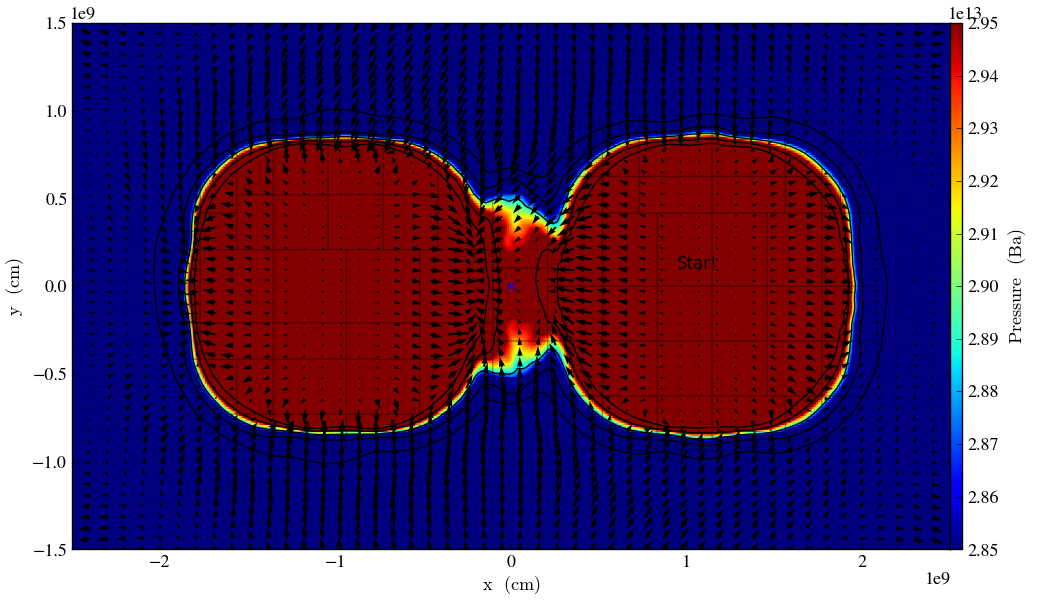
\includegraphics[width=6in]{Slice_z_pressure}
\caption{Pressure slice with annotations}
\end{figure}
%%%%%%%%%%%%%%%%%%%%%%%%%%%%%%%%%

{\it\#------------------------}


{\it\# Volume Rendering}
{\setlength{\parskip}{0pt}

from yt.mods import *
}

pf = load(`plt00020')

field = `pressure'
dd = pf.all\_data()

{\it\# We take the log of the extrema of the pressure field, as well as a couple other interesting}
{\setlength{\parskip}{0pt}

{\it\# value ranges we'd like to visualize.}

h\_mi, h\_ma = dd.quantities[`Extrema'](field)[0]
}

h\_mi, h\_ma = np.log10(h\_mi), np.log10(h\_ma)

s\_mi, s\_ma =  np.log10(2.90e13), np.log10(3.10e13)

pf.index

{\it\# We deal in terms of logarithms here because we have such a large range of values.}
{\setlength{\parskip}{0pt}

{\it\# It can make things easier, but is not necessary.}

pf.field\_info[field].take\_log=True
}

{\it\# This is what we use to visualize volumes. There are a couple of other, more complex}
{\setlength{\parskip}{0pt}

{\it\# ways. We set the range of values we're interested in and the number of bins in the}

{\it\# function. Make sure to have a lot of bins if your data spans many orders of magnitude!}

{\it\# Our raw data ranges from about $10^{13}$ to $10^{22}$.}

tf = ColorTransferFunction((h\_mi-1, h\_ma+1), nbins=1.0e6)
}

{\it\# Here we add several layers to our function, either one at a time or in groups. We}
{\setlength{\parskip}{0pt}

{\it\# specify the value-center and width of the layer. We can manipulate the color by}

{\it\# individually setting the colormaps and ranges to spread them over. We can also}

{\it\# change the transparency, which will usually take some time to get perfect.}

tf.sample\_colormap(np.log10(2.0e21), 0.006, col\_bounds=[h\_mi,h\_ma],
}

{\setlength{\parindent}{96pt}alpha=[27.0], colormap=`RdBu\_r')}

tf.sample\_colormap(np.log10(2.0e19), 0.001, col\_bounds=[h\_mi,h\_ma],

{\setlength{\parindent}{96pt}alpha=[5.5], colormap=`RdBu\_r')}

tf.add\_layers(6, mi=np.log10(2.95e13), ma=s\_ma,

{\setlength{\parindent}{63.5pt}col\_bounds=[s\_mi,s\_ma],}

{\setlength{\parindent}{63.5pt}alpha=19*na.ones(6,dtype=`float64'), colormap=`RdBu\_r')}

tf.sample\_colormap(np.log10(2.95e13), 0.000005, col\_bounds=[s\_mi,s\_ma],

{\setlength{\parindent}{96pt}alpha=[13.0], colormap=`RdBu\_r')}

tf.sample\_colormap(np.log10(2.90e13), 0.000007, col\_bounds=[s\_mi,s\_ma],

{\setlength{\parindent}{96pt}alpha=[11.5], colormap=`RdBu\_r')}

tf.sample\_colormap(np.log10(2.85e13), 0.000008, col\_bounds=[s\_mi,s\_ma],

{\setlength{\parindent}{96pt}alpha=[9.5], colormap=`RdBu\_r')}

{\it\# By default each color channel is only opaque to itself. If  we set grey\_opacity=True,}
{\setlength{\parskip}{0pt}

{\it\# this is no longer the case. This is good to use if we want to obscure the inner}

{\it\# portions of our rendering. Here it only makes a minor change, as we must set our}

{\it\# alpha values for the outer layers higher to see a strong effect.}

tf.grey\_opacity=True
}

{\it\# Volume rendering uses a camera object which centers the view at the coordinates we've}
{\setlength{\parskip}{0pt}

{\it\# called `c.' `L' is the normal vector (automatically normalized) between the camera}

{\it\# position and `c,' and `W' determines the width of the image---again, like a zoom.}

{\it\# `Nvec' is the number of pixels in the x and y directions, so it determines the actual} 

{\it\# size of the image.}

c = [5.0e9, 5.0e9, 5.0e9]
}

L = [0.15, 1.0, 0.40]

W = (pf.domain\_right\_edge - pf.domain\_left\_edge)*0.5

Nvec = 768

{\it\# `no\_ghost' is an optimization option that can speed up calculations greatly, but can}
{\setlength{\parskip}{0pt}

{\it\# also create artifacts at grid edges and affect smoothness.  For our data, there is no}

{\it\# speed difference, so we opt for a better-looking image.}

cam = pf.camera(c, L, W, (Nvec,Nvec), transfer\_function = tf,
}

{\setlength{\parindent}{95pt}fields=[field], pf=pf, no\_ghost=False)}

{\it\# Obtain an image! However, we'll want to annotate it with some other things before}
{\setlength{\parskip}{0pt}

{\it\# saving it.}

im = cam.snapshot()
}

{\it\# Here we draw a box around our stars, and visualize the gridding of the top two levels.}
{\setlength{\parskip}{0pt}

{\it\# Note that draw\_grids returns a new image while draw\_box does not. Also, add\_}

{\it\# background\_color in front of draw\_box is necessary to make the box appear over}

{\it\# blank space (draw\_grids calls this internally). For draw\_box we specify the left}

{\it\# (lower) and right(upper) bounds as well its color and transparency.}

im.add\_background\_color(`black', inline=True)
}

cam.draw\_box(im, np.array([3.0e9, 4.0e9, 4.0e9]),

{\setlength{\parindent}{72pt}np.array([7.0e9, 6.0e9, 6.0e9]), np.array([1.0, 1.0, 1.0, 0.14]))}

im = cam.draw\_grids(im, alpha=0.12, min\_level=2)

im = cam.draw\_grids(im, alpha=0.03, min\_level=1, max\_level=1)

{\it\# `im' is an image array rather than a plot object, so we save it using a different}
{\setlength{\parskip}{0pt}

{\it\# function. There are others, such as `write\_bitmap.'}

im.write\_png(`pressure\_shell\_volume.png')
}
%%%%%%%%%%%%%%%%%%%%%%%%%%%%%%%%%
\begin{figure}[h]
\centering
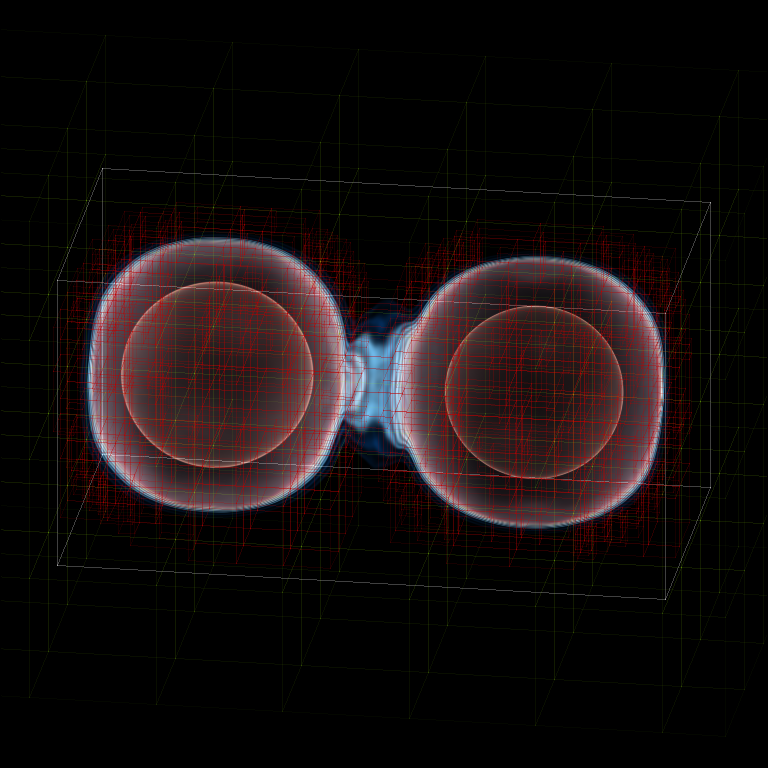
\includegraphics[width=3.5in]{volume}
\caption{Volume rendering}
\end{figure}
%%%%%%%%%%%%%%%%%%%%%%%%%%%%%%%%%


{\it\#------------------------}

{\it\# Isocontour Rendering}
{\setlength{\parskip}{0pt}

{\it\# Here we extract isocontours using some extra modules and plot them using matplotlib.}

from mpl\_toolkits.mplot3d import Axes3D
}

from mpl\_toolkits.mplot3d.art3d import Poly3DCollection

import matplotlib.pyplot as plt

from yt.mods import *

pf = load(`plt00020')

field = `pressure'

field\_weight = `magvel'

contour\_value = 2.83e13

domain = pf.all\_data()

{\it\# This object identifies isocontours at a given value for a given field. It returns}
{\setlength{\parskip}{0pt}

{\it\# the vertices of the triangles in that isocontour. It requires a data source, which}

{\it\# can be an object---but here we just give it all of our data. Here we find a pressure}

{\it\# isocontour and color it the magnitude of velocity over the same contour.}

surface = pf.surface(domain, field, contour\_value)
}

colors = apply\_colormap(np.log10(surface[field\_weight]), cmap\_name=`RdBu')

fig = plt.figure()

ax = fig.gca(projection=`3d')

p3dc = Poly3DCollection(surface.triangles, linewidth=0.0)

p3dc.set\_facecolors(colors[0,:,:]/255.)

ax.add\_collection(p3dc)

{\it\# By setting the scaling on the plot to be the same in all directions (using the x scale),}
{\setlength{\parskip}{0pt}

{\it\# we ensure that no warping or stretching of the data occurs.}

ax.auto\_scale\_xyz(surface.vertices[0,:], surface.vertices[0,:],
}

{\setlength{\parindent}{87pt}surface.vertices[0,:])}

ax.set\_aspect(1.0)

plt.savefig(`pres\_magvel\_isocontours.png')
%%%%%%%%%%%%%%%%%%%%%%%%%%%%%%%%%
\begin{figure}[h]
\centering
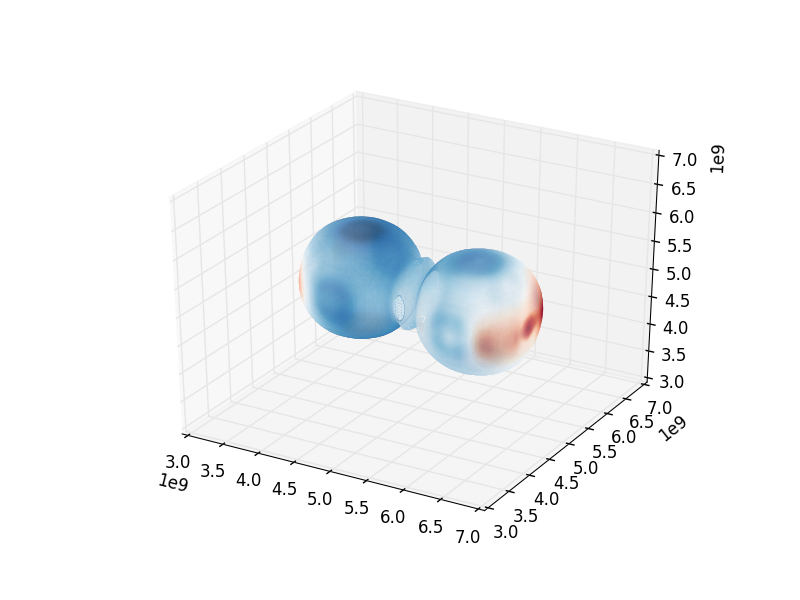
\includegraphics[width=4in]{isocontours}
\caption{Pressure isocontour rendering colored with velocity magnitude}
\end{figure}
%%%%%%%%%%%%%%%%%%%%%%%%%%%%%%%%%

{\it\#------------------------}

{\it\#1-D and 2-D Profiles}
{\setlength{\parskip}{0pt}

{\it\# Line plots and phase plots can be useful for analyzing data in detail.}

from yt.mods import *
}

pf = load(`plt00020')

pf.index

{\it\# Just like with the pressure\_contours script, we can set the units for fields that}
{\setlength{\parskip}{0pt}

{\it\# have none.}

pf.field\_info[`magvel'].\_units = r`\textbackslash rm\{cm\}/\textbackslash rm\{s\}'
}

pf.field\_info[`kineng'].\_units = r`\textbackslash rm\{ergs\}'

{\it\# We can create new fields from existing ones. \yt assumes all units are in cgs, and}
{\setlength{\parskip}{0pt}

{\it\# does not do any unit conversions on its own (but we can make it). Creating new fields}

{\it\#  requires us to define a function that acts on our data and returns the new data,}

{\it\# then call add\_field while supplying the field name, the function the data comes from,}

{\it\# and the units. Here, we create new fields simply to rename our data to make the plot}

{\it\# look prettier.}

def \_newT(field, data):
}

{\setlength{\parindent}{18.5pt}return data[`t']}

add\_field(`X', function=\_newT, units=r`\textbackslash rm\{domain\}\,\textbackslash rm\{fraction\}')

def \_newDen(field, data):

{\setlength{\parindent}{18.5pt}return data[`density']}

add\_field(`Density', function=\_newDen, units=r`\textbackslash rm\{g\}/\textbackslash rm\{cm\}\^{}\{3\}')

{\it\# PlotCollections are one of the most commonly used tools in \yt, alongside SlicePlots and}
{\setlength{\parskip}{0pt}

{\it\# ProjectionPlots. They are useful when we want to create multiple plots from the same}

{\it\# parameter file, linked by common characteristics such as the colormap, its bounds, and}

{\it\# the image width. It is easy to create 1-D line plots and 2-D phase plots through a}

{\it\# PlotCollection, but we can also create thin projections and so on. When we create a}

{\it\# PlotCollection, it is empty, and only requires the parameter file and the 'center' that}

{\it\# will be supplied to plots like slices and sphere plots.}

pc = PlotCollection(pf, `c')
}

{\it\# Now we add a ray---a sample of our data field along a line between two points we define}
{\setlength{\parskip}{0pt}

{\it\# in the function call.}

ray = pc.add\_ray([0.0, 5.0e9, 5.0e9],[1.e10, 5.0e9, 5.0e9], `magvel')
}

{\it\# This is where our derived fields come in handy. Our ray is drawn along the x-axis}
{\setlength{\parskip}{0pt}

{\it\# through the center of the domain, but by default the fraction of the ray we have gone}

{\it\# along is called `t.' We now have the same data in another field we called `X,' whose}

{\it\# name makes more sense, so we'll reassign the ray's first field to be that. If we wanted,}

(\it\# we could also reassign names to `magvel' and `kineng.'

ray.fields = [`X', `magvel']
}

{\it\# Next, we'll create a phase plot. The function requires a data source, and we can't}
{\setlength{\parskip}{0pt}

{\it\# just hand it our parameter file, but as a substitute we can quickly create an object}

{\it\# that spans our entire domain (or use the method in the isocontour example). The}

{\it\#  specifications of the region (a box) are the center, left bound, and right bound.}

region = pf.region([5.0e9, 5.0e9, 5.0e9], [0.0, 0.0, 0.0],
}

{\setlength{\parindent}{100pt}[1.0e10, 1.0e10, 1.0e10])}

{\it\# The phase object accepts a data source, fields, a weight, a number of bins along both}
{\setlength{\parskip}{0pt}

{\it\# axes, and several other things, including its own colormap, logarithm options,}

{\it\# normalization options, and an accumulation option. The first field is binned onto}

{\it\# the x-axis, the second field is binned onto the y-axis, and the third field is}

{\it\# binned with the colormap onto the other two. Subsequent fields go into an underlying}

{\it\# profile and do not appear on the image.}

phase = pc.add\_phase\_object(region, [`Density', `magvel',`kineng'], weight=None,
}

{\setlength{\parindent}{143pt}x\_bins=288, y\_bins=288)}

pc.save(`profile')
%%%%%%%%%%%%%%%%%%%%%%%%%%%%%%%%%
\begin{figure}[h]
  \centering
  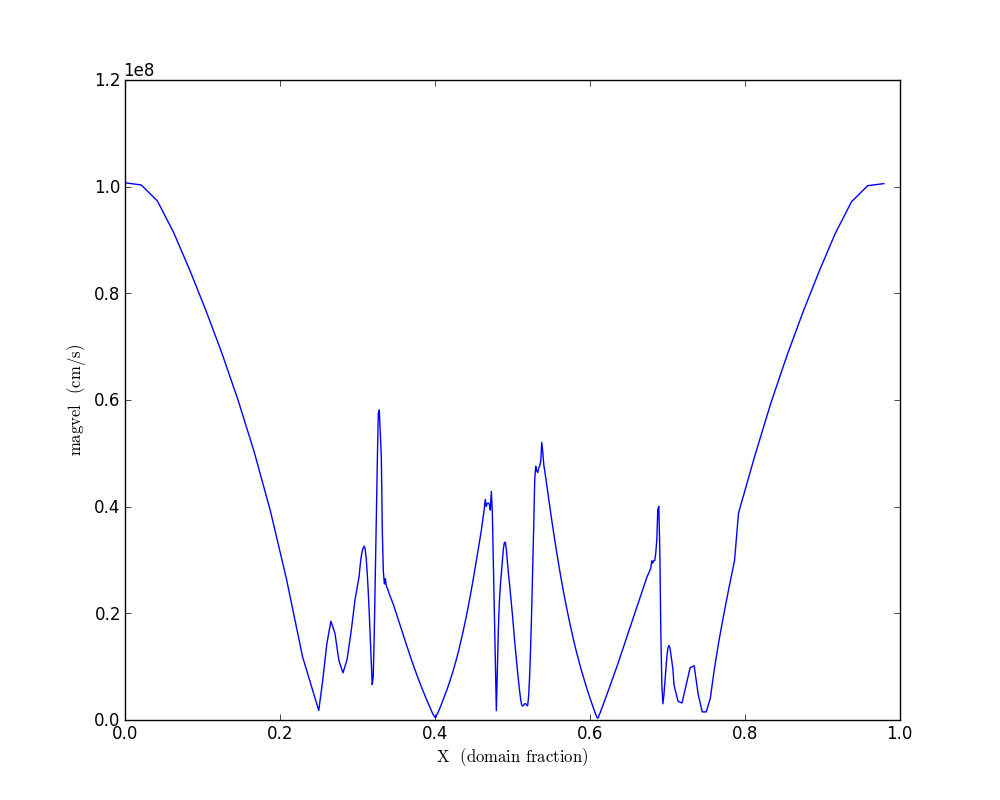
\includegraphics[width=4.0in]{LineQueryPlot_0_t_magvel}
  \caption{1-D velocity magnitude profile}
  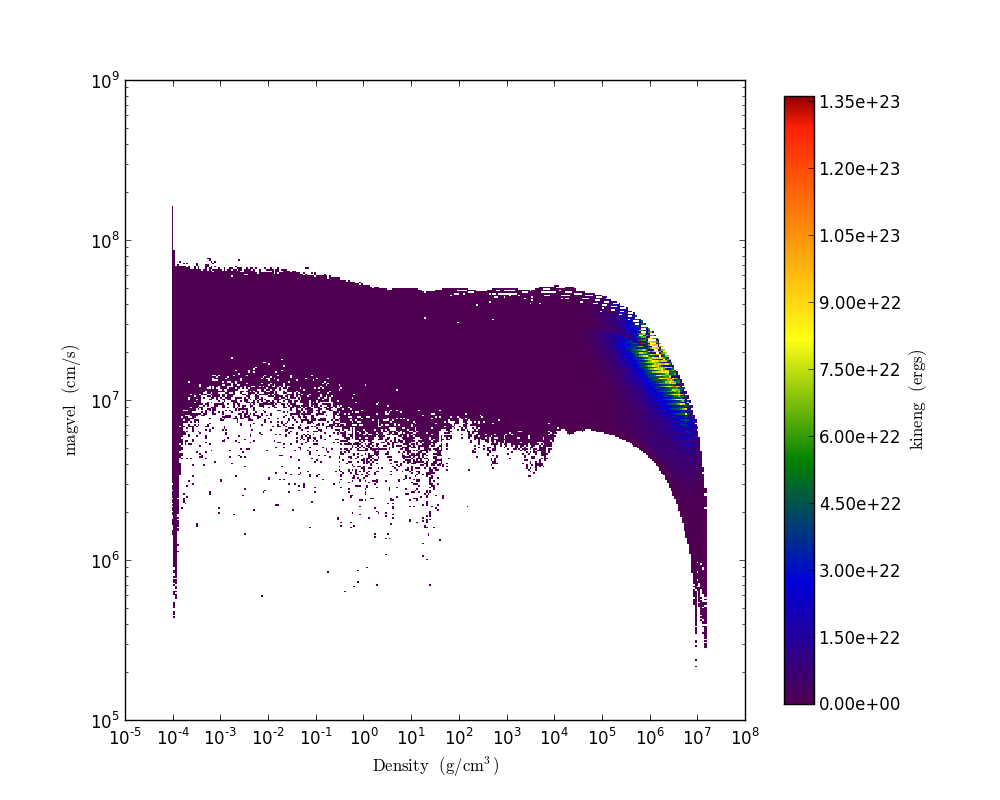
\includegraphics[width=4.0in]{Profile2D_1_Density_magvel_kineng}
  \caption{Density/velocity magnitude/kinetic energy phase plot}
\end{figure}
\quad
%%%%%%%%%%%%%%%%%%%%%%%%%%%%%%%%%

{\it\#------------------------}

{\it\#Off-Axis Projection}
{\setlength{\parskip}{0pt}

{\it\# If we don't want to take a projection (this can be done for a slice as well) along}

{\it\# one of the coordinate axes, we can take one from any direction using an}

{\it\# OffAxisProjectionPlot. To accomplish the task of setting the view up, the plot}

{\it\# requires some of the same parameters as the camera object: a normal vector, center,}

{\it\# width, and field, and optionally we can set no\_ghost (default is False). The normal}

{\it\# vector is automatically normalized as in the case of the camera. The plot also}

{\it\# requires a depth---that is, how much data we want to sample along the line of sight,}

{\it\# centered around the center. In this case `c' is a shortcut for the domain center.}

pf = load(`plt00020')
}

field = `density'

L = [0.25, 0.9, 0.40]

plot = OffAxisProjectionPlot(pf, L, field, center=`c',

{\setlength{\parindent}{146pt}width=(5.0e9, 4.0e9), depth=3.0e9)}

{\it\# Here we customize our newly created plot, dictating the font, colormap, and title.}
{\setlength{\parskip}{0pt}

{\it\# Logarithmic data is used by default for this plot, so we turn it off.}

plot.set\_font(\{`family':`Bitstream Vera Sans', `style':`italic',
}

{\setlength{\parindent}{63.5pt}`weight':`normal', `size':14, `color':`red'\})}

plot.set\_log(field, False)

plot.set\_cmap(field, `jet')

plot.annotate\_title(`Off-Axis Density Projection')

{\it\# The actual size of the image can also be set. Note that the units are in inches.}
{\setlength{\parskip}{0pt}

plot.set\_window\_size(8.0)
}

plot.save(`off\_axis\_density')
%%%%%%%%%%%%%%%%%%%%%%%%%%%%%%%%%
\begin{figure}[h]
  \centering
  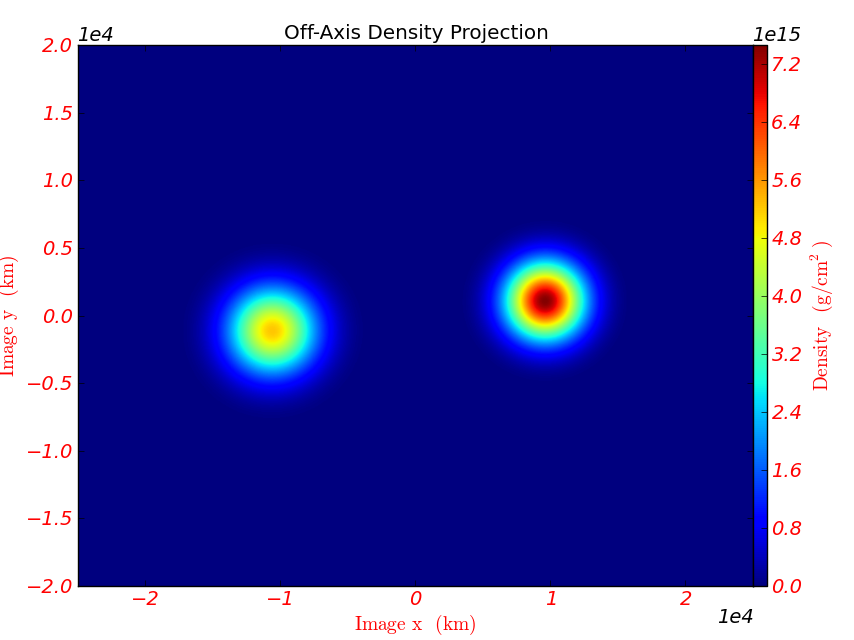
\includegraphics[width=4in]{OffAxisProjection_density}
  \caption{Off-axis density projection}
\end{figure}
%%%%%%%%%%%%%%%%%%%%%%%%%%%%%%%%%




\chapter{Verification Test Problems}
\input{Verification/Verification.tex}


%------------------------------------------------------------------------------
\backmatter

\renewcommand\bibname{References}
\addcontentsline{toc}{chapter}{References}
\bibliographystyle{plain}
\bibliography{refs,Verification/verification,Gravity/gr}

\cleardoublepage
\phantomsection
\addcontentsline{toc}{chapter}{Index}
\printindex

\end{document}
